%!TEX program = xelatex
\documentclass[dvipsnames, svgnames,a4paper,11pt]{article}
% ----------------------------------------------------- 
%	加边框的命令
%	参考:https://tex.stackexchange.com/questions/531559/how-to-add-the-page-border-for-first-two-pages-in-latex
\usepackage{tikz}
\usetikzlibrary{calc}
\usepackage{eso-pic}
\AddToShipoutPictureBG{%
\begin{tikzpicture}[overlay,remember picture]
\draw[line width=0.6pt] % 边框粗细
    ($ (current page.north west) + (0.6cm,-0.6cm) $)
    rectangle
    ($ (current page.south east) + (-0.6cm,0.6cm) $); % 边框位置
\end{tikzpicture}}


\usepackage{xcolor}
\definecolor{c1}{HTML}{070F94} % 目录颜色 原版为2752C9 紫灰色535AAA 蓝紫色0B0DB7 深蓝色070F94 湖绿色219394 松石灰绿086173
\definecolor{c2}{HTML}{E20129} % 引用颜色 原版\definecolor{c2}{RGB}{190,20,83} 橙色F24729

\usepackage{ctex}
\usepackage[top=28mm,bottom=28mm,left=15mm,right=15mm]{geometry}
\usepackage{hyperref} 
\hypersetup{
	colorlinks,
	linktoc = section, % 超链接位置,选项有section, page, all
	linkcolor = c1, % linkcolor 目录颜色
	citecolor = c1  % citecolor 引用颜色
}
\usepackage{amsmath,enumerate,multirow,float}
\usepackage{tabularx}
\usepackage{tabu}
\usepackage{subfig}
\usepackage{fancyhdr}
\usepackage{graphicx}
\usepackage{wrapfig}  
\usepackage{physics}
\usepackage{appendix}
\usepackage{amsfonts}

%
\usepackage{tcolorbox}
\tcbuselibrary{skins,breakable}
\newtcolorbox{tbox}[2][]{
    colframe=black!70!,
    breakable,
    enhanced,
	boxrule =0.5pt,
    title = {#2},
    fonttitle = \large\kaishu\bfseries,
	drop fuzzy shadow,
    #1
}
\newtcolorbox[auto counter,number within=section]{question}[1][]{
  top=2pt,bottom=2pt,arc=1mm,
  boxrule=0.5pt,
%   frame hidden,
  breakable,
  enhanced, %跨页后不会显示下边框
  coltitle=c1!80!gray,
  colframe=c1,
  colback=c1!3!white,
  drop fuzzy shadow,
  title={思考题~\thetcbcounter:\quad},
  fonttitle=\bfseries,
  attach title to upper,
  #1
}

% ---------------------------------------------------------------------
%	利用cleveref改变引用格式,\cref是引用命令
\usepackage{cleveref}
\crefformat{figure}{#2{\textcolor{c2}{Figure #1}}#3} % 图片的引用格式
\crefformat{equation}{#2{(\textcolor{c2}{#1})}#3} % 公式的引用格式
\crefformat{table}{#2{\textcolor{c2}{Table #1}}#3} % 表格的引用格式


% ---------------------------------------------------------------------
%	页眉页脚设置
\fancypagestyle{plain}{\pagestyle{fancy}}
\pagestyle{fancy}
\lhead{\kaishu 中山大学物理与天文学院基础物理实验\uppercase\expandafter{\romannumeral2}} % 左边页眉,学院 + 课程
\rhead{\kaishu 实验报告By黄罗琳} % 右边页眉,实验报告标题
\cfoot{\thepage} % 页脚,中间添加页码


% ---------------------------------------------------------------------
%	对目录、章节标题的设置
\renewcommand{\contentsname}{\centerline{\huge 目录}}
\usepackage{titlesec}
\usepackage{titletoc}
% \titleformat{章节}[形状]{格式}{标题序号}{序号与标题间距}{标题前命令}[标题后命令]
\titleformat{\section}{\centering\LARGE\songti}{}{1em}{}

% ---------------------------------------------------------------------
%   listing代码环境设置
\usepackage{listings}
\lstloadlanguages{python}
\lstdefinestyle{pythonstyle}{
backgroundcolor=\color{gray!5},
language=python,
frameround=tftt,
frame=shadowbox, 
keepspaces=true,
breaklines,
columns=spaceflexible,                   
basicstyle=\ttfamily\small, % 基本文本设置,字体为teletype,大小为scriptsize
keywordstyle=[1]\color{c1}\bfseries, 
keywordstyle=[2]\color{Red!70!black},   
stringstyle=\color{Purple},       
showstringspaces=false,
commentstyle=\ttfamily\scriptsize\color{green!40!black},%注释文本设置,字体为sf,大小为smaller
tabsize=2,
morekeywords={as},
morekeywords=[2]{np, plt, sp},
numbers=left, % 代码行数
numberstyle=\it\tiny\color{gray}, % 代码行数的数字字体设置
stepnumber=1,
rulesepcolor=\color{gray!30!white}
}




% ---------------------------------------------------------------------
%	其他设置
\def\degree{${}^{\circ}$} % 角度
\graphicspath{{./images/}} % 插入图片的相对路径
\allowdisplaybreaks[4]  %允许公式跨页 
\usepackage{lipsum}
\usepackage{enumitem}
\usepackage{tabularray}  %绘制表格时可以更加方便添加框线
\usepackage{xcolor} %添加更多文本颜色
%\usepackage{mathrsfs} % 字体
%\captionsetup[figure]{name=Figure} % 图片形式
%\captionsetup[table]{name=Table} % 表格形式
\begin{document}
	
	% 实验报告封面	
	% 顶栏
	\begin{table}
		\renewcommand\arraystretch{1.7}
		\begin{tabularx}{\textwidth}{
			|>{\centering}X|>{\centering}X|>{\centering}X
			|>{\centering}X|>{\centering}X|>{\centering\arraybackslash}X|}
		\hline
		\multicolumn{2}{|c|}{预习报告}&\multicolumn{2}{c|}{实验记录与分析}&\multicolumn{2}{c|}{总成绩}\\
		\hline
		\LARGE30 & & \LARGE50 & & \LARGE80 & \\
		\hline
		\end{tabularx}
	\end{table}
	
	
	\begin{table}
		\renewcommand\arraystretch{1.7}
		\begin{tabularx}{\textwidth}{|X|X|X|X|}
		\hline
		年级、专业:& 物理学 &组号:& 实验班1\\
		\hline
		姓名:& 黄罗琳、丁侯凯 & 学号: & 2344001、22344010 \\
		\hline
		日期:& 2024/05/23 & 教师签名:& \\
		\hline
		\end{tabularx}
	\end{table}
	
	\begin{center}
		\LARGE TEC控温实验
	\end{center}
	
	\textbf{【实验报告注意事项】}
	\begin{enumerate}[label=\arabic*., leftmargin=*]
		\item 实验报告由两部分组成:
			\begin{enumerate}[label=\arabic*), leftmargin=*]
				\item 预习报告:课前认真研读\underline{\textbf{实验讲义}},弄清实验原理;实验所需的仪器设备、用具及其使用、完成课前预习思考题;了解实验需要测量的物理量,并根据要求提前准备实验记录表格(可以参考实验报告模板,可以打印)。\textcolor{red}{\textbf{(30分)}}
				\item 实验记录与分析:认真、客观记录实验条件、实验过程中的现象以及数据。实验记录请用珠笔或者钢笔书写并签名(\textcolor{red}{\textbf{用铅笔记录的被认为无效}})。\textcolor{red}{\textbf{保持原始记录,包括写错删除部分,如因误记需要修改记录,必须按规范修改。}}(不得手记的值输入到电脑打印);离开前请实验教师检查记录并签名。\textcolor{red}{\textbf{(50分)}}
			\end{enumerate}
		
		\item \textcolor{red}{\textbf{本实验报告可提前打印出来,当场记录分析完成交给带实验的老师,课后无需再提交。若当场完成不了,则请课后完成,再扫描并通过seelight提交。}}
		
		\textcolor{red}{\textbf{注意:本文档已留出填写空间,若填写空间不够的话请提前规划留白,做到报告的美观}}
		\item 注意事项:
			\begin{enumerate}[label=\arabic*), leftmargin=*]
				\item 本实验电路比较复杂, 需要耐心连接, 认真检查。
				\item 程序编写和调试过程中, 遇到问题及时查看 LabVIEW 帮助, 留意各个器件时刻处于可
				控状态。
				\item 直流稳压电源的输出,要根据实验过程及时地手动打开或关闭,不要在程序没有正常
				运行的情况下,让直流稳压电源有持续的输出。
				\item 注意根据信号电流大小选取合适直接的导线, 杜邦线一般只用于小电流和信号传输,
				电流大时则需要选用直径大的导线。
			\end{enumerate}
	\end{enumerate}
	
	
	\clearpage
	\tableofcontents
	\clearpage
	
	\setcounter{section}{0}
	\section{TEC控温实验 \quad\heiti 预习报告}
		
	\subsection{实验目的}
		\begin{enumerate}
			\item 了解 TEC 半导体控温的原理和PID 参数的调节。
			\item 基于 LabVIEW 和 myDAQ 设计和搭建温度采集和控制系统。
			
			
		\end{enumerate}
	
	\subsection{仪器用具}
	\begin{table}[h!]
		\centering
		\begin{tabular}{|c|m{4cm}|c|m{8cm}|}
		\hline
		编号 & 仪器用具名称 & 数量 & 主要参数(型号,量程,测量精度等) \\ 
		\hline
		1 & 计算机 & 1 & Windows 系统,安装 LabVIEW 程序 \\ 
		\hline
		2 & myDAQ & 1 &  \\ 
		\hline
		3 & 直流稳压电源 & 1 & DP832 \\ 
		\hline
		4 & 控温实验平台 & 1 & 12V 供电,最大电流 2A \\ 
		\hline
		5 & IBT\_2 电机驱动器 & 1 & 24V 供电,测温范围 0-100℃,输出电压 0-10V \\ 
		\hline
		6 & 温度变送器 & 1 &  \\ 
		\hline
		7 & 电路元器件 & 1 & 面包板,连接线等 \\ 
		\hline
		\end{tabular}
		\caption{仪器用具清单}
		\end{table}
	
	\subsection{原理概述}
	\begin{enumerate}
	\item \textbf{PID反馈控制原理}
	
	PID控制器是最常见的反馈控制器之一,广泛应用于工业控制系统。PID是比例(Proportional)、积分(Integral)和微分(Derivative)三种控制方式的缩写。PID控制器的目标是使输出尽可能接近设定值,通过调节控制输入来减少误差。以下是PID控制器的基本原理:
	\begin{figure}[{H}]
		\centering
		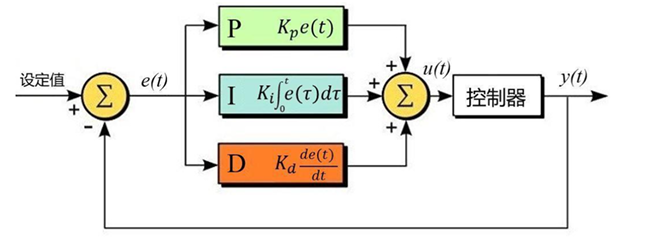
\includegraphics[width=0.5\linewidth]{原理.png}
		\caption{PID反馈控制原理}
		\label{}
	\end{figure}

\subsubsection*{ 比例控制(P控制)}
比例控制是控制器的基本部分。比例控制器通过将当前误差(设定值与实际值的差)乘以比例系数\(K_p\)来计算控制输出。依赖于当前误差。 比例控制与误差信号成比例,较大的比例增益可以对误
差信号有更大的响应。比例增益太高会使电路在目标值附近振荡;比例增益太低,电路将不能有效
地对系统变化进行响应。

\[
u(t) = K_p \cdot e(t)
\]

其中:
\begin{itemize}
    \item \(u(t)\) 是控制输出
    \item \(e(t) = r(t) - y(t)\) 是误差,\(r(t)\) 是设定值,\(y(t)\) 是实际输出
    \item \(K_p\) 是比例增益
\end{itemize}

\subsubsection*{积分控制(I控制)}

积分控制通过对误差随时间的累积进行积分,消除稳态误差。积分控制器的输出与误差的积分成正比。积分增益过高,会引起电路
的过度超调,从而导致振荡和不稳定;积分增益太低,电路在系统发生改变时响应将十分缓慢。

\[
u(t) = K_i \int_{0}^{t} e(\tau) d\tau
\]

其中:
\begin{itemize}
    \item \(K_i\) 是积分增益
\end{itemize}

\subsubsection*{ 微分控制(D控制)}

微分控制通过对误差的变化率进行微分,预测误差的变化趋势,改善系统的动态响应。微分控制增益过高,会使电路响应速度非常缓慢,并使电路对噪声和高
频振荡非常敏感;微分控制增益太低,电路则很有可能发生设定值的超调。但是在一些情况下,如果需要避免任何程度的设定值超调,就应该采用更高的微分增益。

\[
u(t) = K_d \frac{de(t)}{dt}
\]

其中:
\begin{itemize}
    \item \(K_d\) 是微分增益
\end{itemize}

\subsection*{PID控制器的综合输出}

PID控制器将上述三部分控制作用相加,得到最终的控制输出:

\[
u(t) = K_p e(t) + K_i \int_{0}^{t} e(\tau) d\tau + K_d \frac{de(t)}{dt}
\]

综合来看,PID控制器可以同时调整比例、积分和微分增益,以实现对系统的精确控制。比例控制主要影响系统的响应速度,积分控制消除稳态误差,而微分控制则改善系统的动态性能。

\item 半导体控温原理(Peltier 效应、 Seebeck 效应、以及两者之间的关系)

半导体控温原理主要依赖于Peltier效应和Seebeck效应,这两种效应都是热电效应的一部分,广泛应用于温度控制和温差发电。以下是对这两种效应及其关系的解释。

\subsubsection*{1. Peltier效应}
Peltier效应指的是当电流通过两种不同的导体或半导体连接形成的接点时,接点处会吸收或释放热量。这种效应可以用来实现温度控制,例如在Peltier制冷片中应用。

当直流电流通过连接在一起的两种不同半导体(n型和p型)时,在一个接点会吸收热量(制冷效果),而在另一个接点会释放热量(加热效果)。这种效应的热量变化与电流成正比。

\[
Q = \Pi \cdot I
\]

其中:
\begin{itemize}
    \item \(Q\) 是吸收或释放的热量
    \item \(\Pi\) 是Peltier系数
    \item \(I\) 是电流
\end{itemize}

\subsubsection*{2. Seebeck效应}
Seebeck效应指的是当两种不同的导体或半导体连接形成回路并存在温差时,会在回路中产生电动势。这种效应可以用来实现温差发电。

当两个不同半导体(n型和p型)连接形成闭合回路并存在温差\(\Delta T\)时,在回路中会产生电动势(电压)。

\[
V = S \cdot \Delta T
\]

其中:
\begin{itemize}
    \item \(V\) 是产生的电动势
    \item \(S\) 是Seebeck系数
    \item \(\Delta T\) 是温差
\end{itemize}

\subsubsection*{3. Peltier效应与Seebeck效应的关系}
Peltier效应和Seebeck效应是热电效应的两个不同表现形式,但它们之间有着密切的关系,都是热电材料的基本性质。

\begin{itemize}
    \item 在Peltier效应中,电流通过不同材料的接点引起热量的吸收或释放。
    \item 在Seebeck效应中,温差引起不同材料的接点产生电动势。
\end{itemize}

两者的关系可以通过热电材料的性能参数联系起来,Peltier系数\(\Pi\)和Seebeck系数\(S\)之间有如下关系:

\[
\Pi = S \cdot T
\]

其中:
\begin{itemize}
    \item \(T\) 是绝对温度
\end{itemize}

这种关系说明了在一定温度下,Peltier效应和Seebeck效应是等效的,反映了热电材料在能量转换中的对偶性。
\item 傅里叶变换基本原理,功率谱密度或幅度谱密度基本原理

傅里叶级数:傅里叶级数表示周期函数可以用正弦和余弦函数的无限级数来表示,其中\(f(x)\)表示周期为\(2\pi\)的函数。
\begin{align*}
	&f(x)=\frac{a_{0}}{2}+\sum_{n=1}^{\infty}a_{n}\cos(nx)+\sum_{n=1}^{\infty}b_{n}\sin(nx)  \\
	&f(t)=\int_{-\infty}^{\infty}f(t)e^{-i\omega t}dt\int_{-\infty}^{\infty}e^{i\omega t}d\omega  \\
	&\text{傅里叶变换:傅里叶变换将一个函数从时域转换到频域,\(F(k)\)表示在频域\(k\)处的频谱分量。} \\
	&F(k )=\int_{-\infty}^{\infty}f(x)e^{-ikx}dx  \\
	&F(\omega  )=\int_{-\infty}^{\infty}f(t)e^{-i\omega t}dt  \\
	&\text{傅里叶逆变换:傅里叶逆变换用于将频域信号恢复到时域。} \\
	&f(t)=\frac{1}{2\pi}\int_{-\infty}^{\infty}F(\omega)e^{i\omega t}d\omega   \\
	&\text{能量守恒:能量守恒表明信号在时域和频域之间的能量是相等的。} \\
	&\int_{-\infty}^{\infty}|f(t)|^{2}dt=\frac{1}{2\pi}\int_{-\infty}^{\infty}|F(\omega)|^{2}d\omega=\int_{-\infty}^{\infty}|F(f)|^{2}df \\
	&\text{功率P:功率\(P\)表示信号的平均功率,\(S(f)\)表示功率谱密度(PSD),描述信号在不同频率上的功率分布。} \\
	&P=\lim_{T\to\infty}\frac{1}{T}\int_{-T/2}^{T/2}E[|f(t)|^{2}]dt=\int_{-\infty}^{\infty}S(f)df \\
	&\text{功率谱密度PSD} \\
	&S(f)=\lim_{T\to\infty}\frac{E[|F_{T}(f)|^{2}]}{T}  \\
	&\text{幅度谱密度ASD:幅度谱密度(ASD)是PSD的平方根,用于表示信号在不同频率上的振幅。} \\
	&\text{ASD}=\sqrt{PSD} 
	\end{align*}
	
	

\end{enumerate}
	
		
	
	
	\subsection{实验前思考题}
		\begin{question}
			热敏电阻测温点位置不同, 是否会影响PID 参数的设定, 为什么?
		\end{question}
			
		测温点位置的不同会导致对控温装置的响应延迟不同,距离温度控制装置(如TEC,热电冷却器)越远的测温点,其响应延迟通常会更大。这是因为温度变化需要一定的时间传播到测温点处,然后才能被传感器检测到。这种响应延迟会影响到控温系统的性能,特别是PID控制器的参数设定。

当测温点位置离控温装置较远时,其对温度变化的响应速度较慢,导致控温装置难以及时作出反应,从而影响到温度的稳定性和控制精度。在PID控制器的参数设定中,需要考虑到这种响应延迟,以调整控制器的响应速度和稳定性。通常情况下,当测温点位置距离控温装置较远时,可能需要增加PID控制器的比例增益(P)、积分时间(I)和微分时间(D),以提高系统的响应速度和稳定性,从而更好地实现温度控制的要求。
			
			
			
			
	
		\begin{question}
			被控物体材料不同, 是否会影响PID 参数的设定, 为什么?
		\end{question} 
			
		被控物体的材料不同会导致其热学性质不同,例如热容量、导热系数等,进而影响其升温速度、冷却速度以及对温度变化的响应速度。这些因素会直接影响到PID控制器参数的设定。

热容量:不同材料的热容量可能不同,热容量越大的物体在升温和降温时需要吸收或释放更多的热量,因此会导致更长的响应时间。在PID控制器的参数设定中,需要考虑到物体的热容量,适当调整积分时间(I),以确保系统的稳定性和控制精度。

导热系数:不同材料的导热系数也不同,高导热系数的物体会更快地传导温度变化,因此具有更快的响应速度。在PID控制器的参数设定中,需要考虑到物体的导热性,适当调整比例增益(P)和微分时间(D),以提高系统的响应速度。

综合来看,被控物体材料不同会导致其对控温的响应速度不同,进而影响到PID控制器参数的设定。为了实现良好的温度控制效果,需要根据被控物体的热学性质调整PID参数,以适应不同的工作条件和控制要求。
	
\begin{question}
	除了脉冲宽度调制控温, 可以使用连续信号控温吗? 如何实现?
\end{question}
连续信号控温方法及其实现方式

\subsection*{模拟电压控制}

通过调节模拟电压信号来控制加热器或制冷器的输出功率。这种方法通常使用运算放大器和线性调节器进行控制。

\paragraph*{关键组件:}
\begin{itemize}
    \item \textbf{电压源}:提供可调节的电压信号。
    \item \textbf{线性调节器}:调整输出功率以匹配输入的模拟电压信号。
    \item \textbf{温度传感器}:测量当前温度并将信号反馈给控制器。
    \item \textbf{PID控制器}:根据温度反馈信号调整输出电压,实现温度控制。
\end{itemize}

\paragraph*{实现步骤:}
\begin{enumerate}
    \item 将温度传感器连接到PID控制器,以测量当前温度。
    \item PID控制器根据设定的目标温度计算误差,并输出相应的控制电压信号。
    \item 线性调节器根据PID控制器输出的控制电压信号调整加热器或制冷器的功率。
    \item 温度传感器实时测量温度,并将反馈信号传递给PID控制器,形成闭环控制。
\end{enumerate}

\subsection*{模拟电流控制}

通过调节模拟电流信号来控制加热器或制冷器的输出功率。这种方法通常使用电流源和电流控制器进行控制。

\paragraph*{关键组件:}
\begin{itemize}
    \item \textbf{电流源}:提供可调节的电流信号。
    \item \textbf{电流控制器}:调整输出功率以匹配输入的模拟电流信号。
    \item \textbf{温度传感器}:测量当前温度并将信号反馈给控制器。
    \item \textbf{PID控制器}:根据温度反馈信号调整输出电流,实现温度控制。
\end{itemize}

\paragraph*{实现步骤:}
\begin{enumerate}
    \item 将温度传感器连接到PID控制器,以测量当前温度。
    \item PID控制器根据设定的目标温度计算误差,并输出相应的控制电流信号。
    \item 电流控制器根据PID控制器输出的控制电流信号调整加热器或制冷器的功率。
    \item 温度传感器实时测量温度,并将反馈信号传递给PID控制器,形成闭环控制。
\end{enumerate}

\subsection*{线性放大器控制}

使用线性放大器(如晶体管或运算放大器)来调节加热器或制冷器的功率输出。这种方法提供平滑的控制信号,减少功率损耗。

\paragraph*{关键组件:}
\begin{itemize}
    \item \textbf{线性放大器}:放大控制信号并驱动加热器或制冷器。
    \item \textbf{温度传感器}:测量当前温度并将信号反馈给控制器。
    \item \textbf{PID控制器}:根据温度反馈信号调整输出信号,实现温度控制。
\end{itemize}

\paragraph*{实现步骤:}
\begin{enumerate}
    \item 将温度传感器连接到PID控制器,以测量当前温度。
    \item PID控制器根据设定的目标温度计算误差,并输出相应的控制信号。
    \item 线性放大器根据PID控制器输出的控制信号调整加热器或制冷器的功率。
    \item 温度传感器实时测量温度,并将反馈信号传递给PID控制器,形成闭环控制。
\end{enumerate}


连续信号控温方法通过调节电压或电流来精确控制温度。这些方法包括模拟电压控制、模拟电流控制和线性放大器控制,均可实现高效、稳定的温度控制。关键在于合理设置PID参数和反馈机制,以确保系统稳定运行。

	% 实验记录	
	\clearpage
	
	% 顶栏
	\begin{table}
		\renewcommand\arraystretch{1.7}
		\centering
		\begin{tabularx}{\textwidth}{|X|X|X|X|}
			\hline
			专业: & 物理学 & 年级: & 2022级 \\
			\hline
			姓名: & 黄罗琳、丁侯凯 & 学号: &22344001、22344010 \\
			\hline
			室温: &26℃  & 实验地点: & A515 \\
			\hline
			学生签名:&
\includegraphics[width=1cm]{签字.jpg} 
\includegraphics[width=1cm]{dhk.png}  & 评分: &\\
			\hline
			实验时间:& 2024/5/23 & 教师签名:&\\
			\hline
		\end{tabularx}
	\end{table}
	% ---
	
	% 小标题
	\section{TEC控温实验  \quad\heiti 实验记录}
	% ---
	
	% 实验过程记录
	\subsection{实验电路连接}
	\begin{figure}[H]
		\centering
		\begin{minipage}[b]{0.45\textwidth}
			\centering
			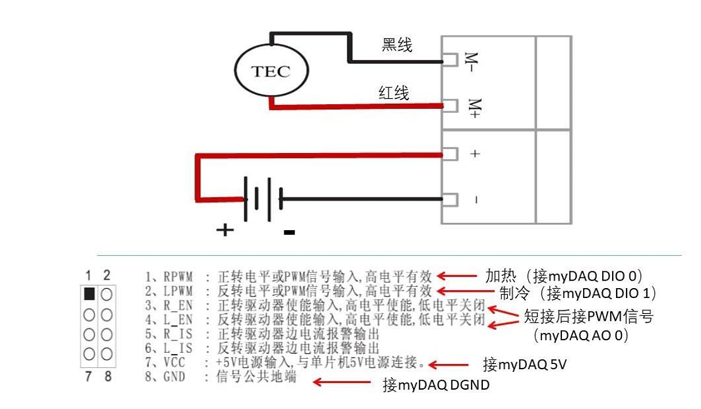
\includegraphics[width=\textwidth]{电路示意.png}
			\caption{接线示意图}
			\label{fig:接线示意图}
		\end{minipage}
		\hspace{1cm}
		\begin{minipage}[b]{0.45\textwidth}
			\centering
			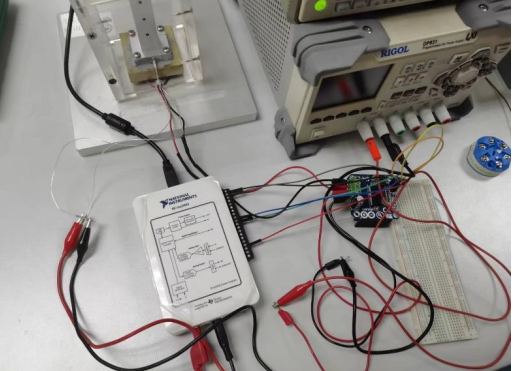
\includegraphics[width=\textwidth]{连接.png}
			\caption{电路连接}
			\label{fig:电路连接}
		\end{minipage}
	\end{figure}
	\subsection{Labview编程截图}
	
	\begin{figure}[{H}]
		\centering
		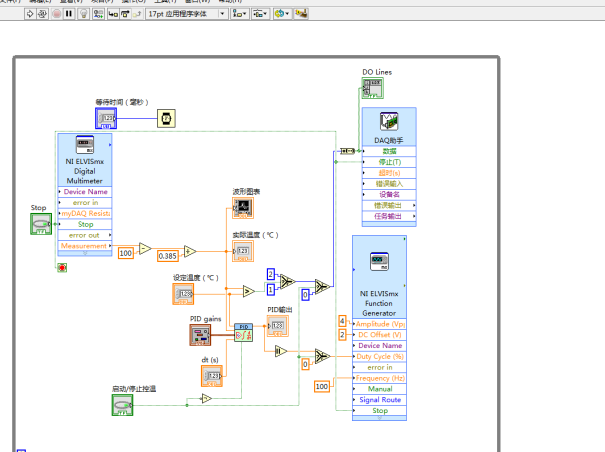
\includegraphics[width=0.4\linewidth]{程序.png}
		\caption{编程截图}
		\label{}
	\end{figure}
	% ---
	
	% 原始数据
	\clearpage
	
	% ---
	
	% 问题记录
	\subsection{控温结果截图}
	\begin{enumerate}
		\item 25摄氏度PI
		
\begin{figure}[{H}]
	\centering
	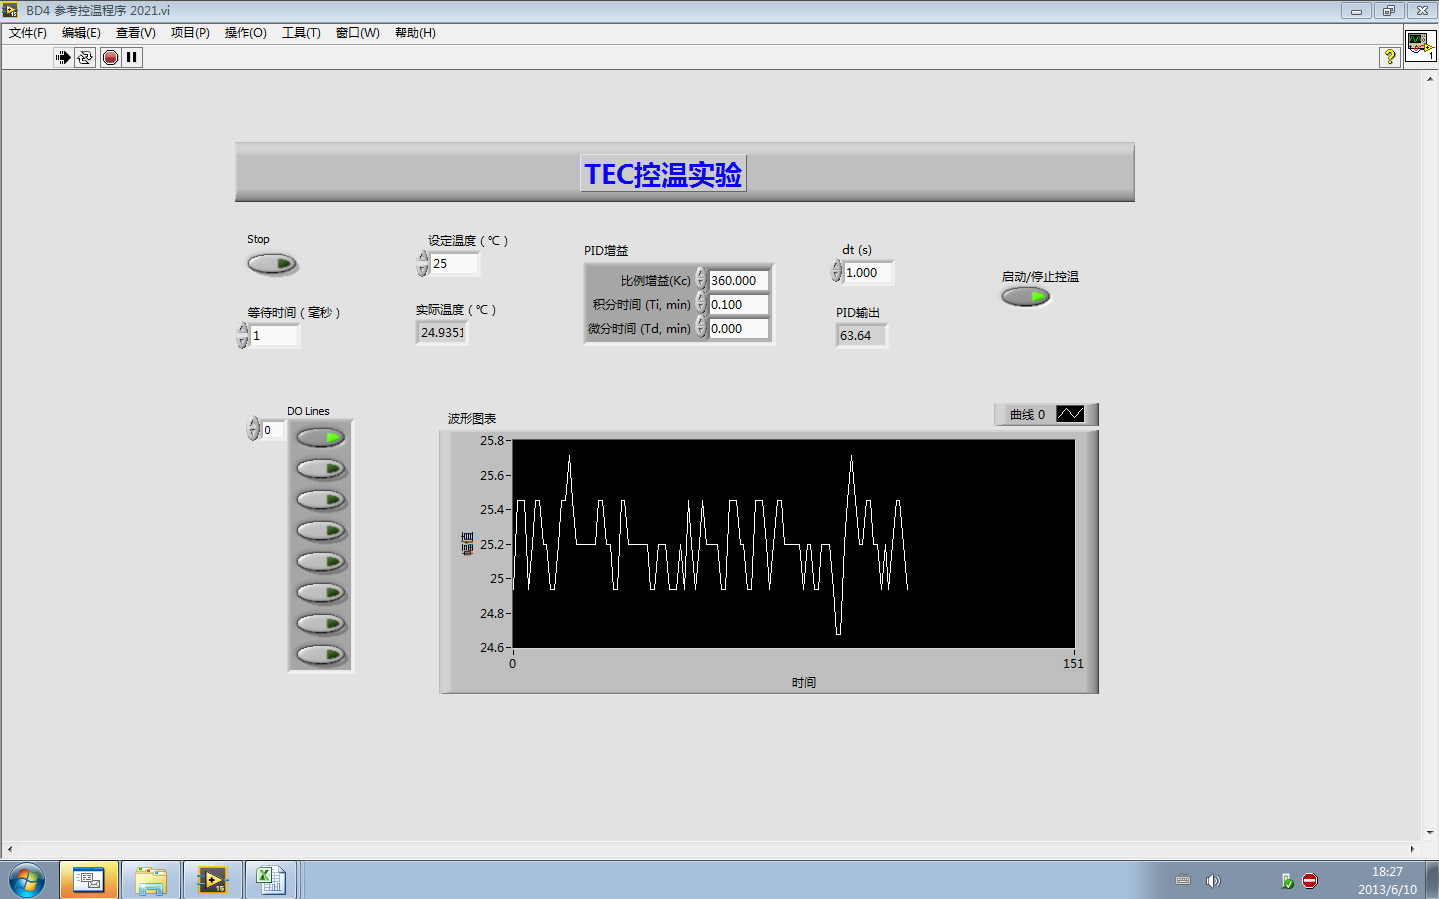
\includegraphics[width=0.8\linewidth]{黄丁稳定温度25 PI.PNG}
	\caption{25℃控温}
	\label{}
\end{figure}
\item 25摄氏度PID
\begin{figure}[{H}]
	\centering
	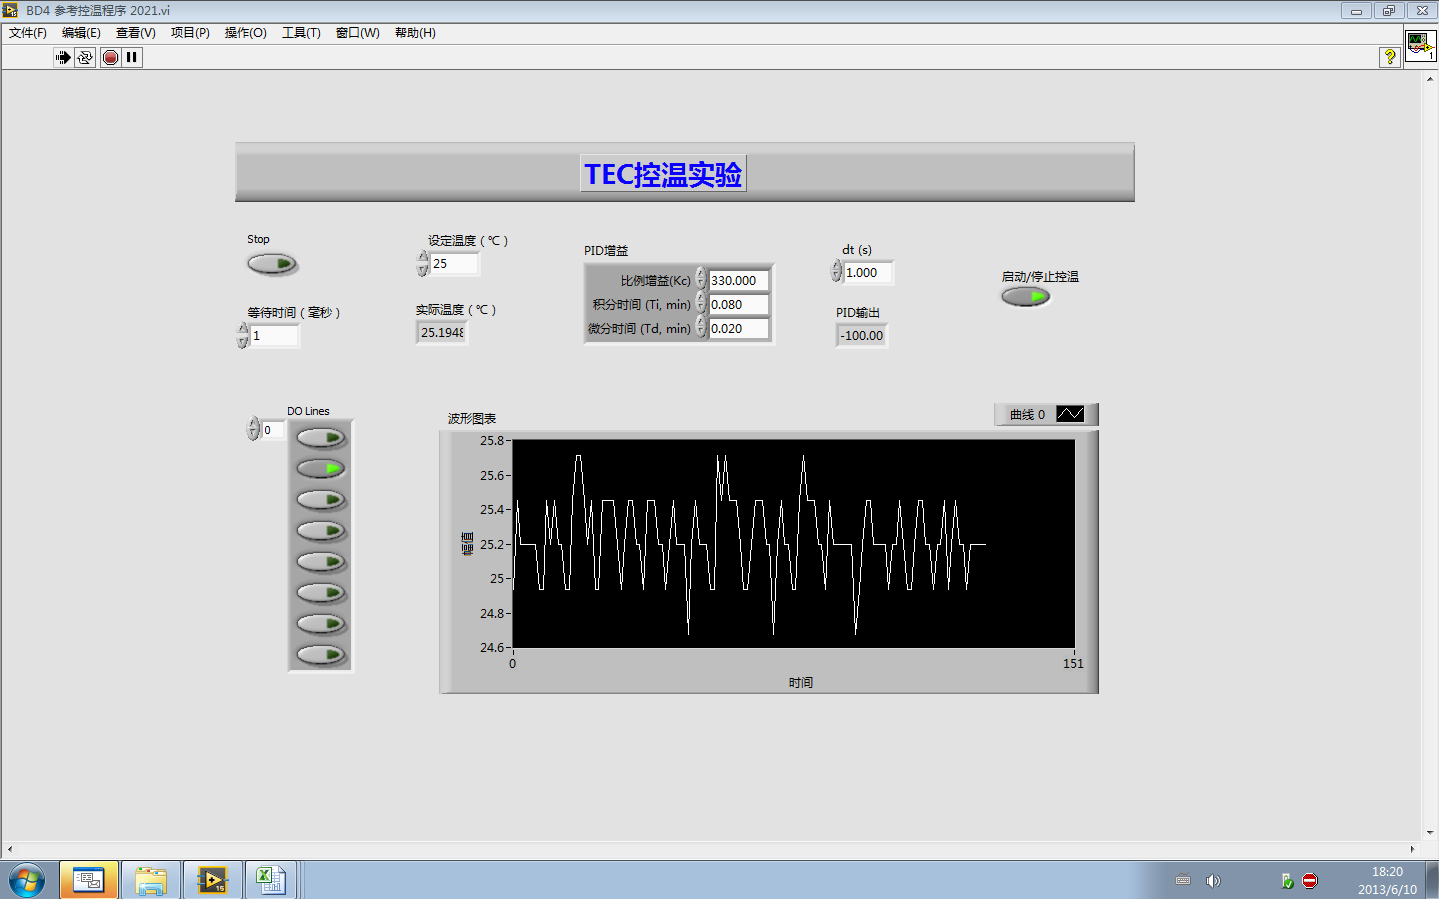
\includegraphics[width=0.8\linewidth]{黄丁实验图象.PNG}
	\caption{25℃控温PID}
	\label{}
\end{figure}
	\end{enumerate}
	\subsection{实验数据}
	\begin{table}[!ht]
		\centering
		\begin{tabular}{|l|l|l|l|l|l|l|}
		\hline
			实验组 & 设定温度 & 实际温度(平均) & 控温时长 & KP & KI & Kd \\ \hline
			P1 & 25 & 25.21 & 75 & 620 & 0 & 0 \\ \hline
			P2 & 33 & 33.05 & 175 & 600 & 0 & 0 \\ \hline
			PI1 & 25 & 25.25 & 112 & 380 & 0.1 & 0 \\ \hline
			PI2 & 33 & 33.29 & 63 & 360 & 0.6 & 0 \\ \hline
			PID1 & 25 & 25.24 & 70 & 330 & 0.08 & 0.02 \\ \hline
			PID2 & 33 & 33.21 & 225 & 300 & 0.067 & 0.02 \\ \hline
		\end{tabular}
	\end{table}
	
	
	
	% 分析与讨论	
	\clearpage
	
	% 顶栏
	\begin{table}
		\renewcommand\arraystretch{1.7}
		\begin{tabularx}{\textwidth}{|X|X|X|X|}
			\hline
			专业:& 物理学 &年级:& 2022级\\
			\hline
			姓名: &  黄罗琳、丁侯凯& 学号:&22344001、22344010 \\
			\hline
			日期:&  2024/5/23& 评分: &\\
			\hline
		\end{tabularx}
	\end{table}
	% ---
	
	% 小标题
	\section{TEC控温实验\quad\heiti 分析与讨论}
	% ---
	
	% 数据处理
	\subsection{实验数据绘图}
	\subsubsection{数据时域图}
	以下所有关于温度的时域图纵坐标单位为摄氏度(℃),横坐标为秒(S)
	\begin{figure}[{H}]
		\centering
		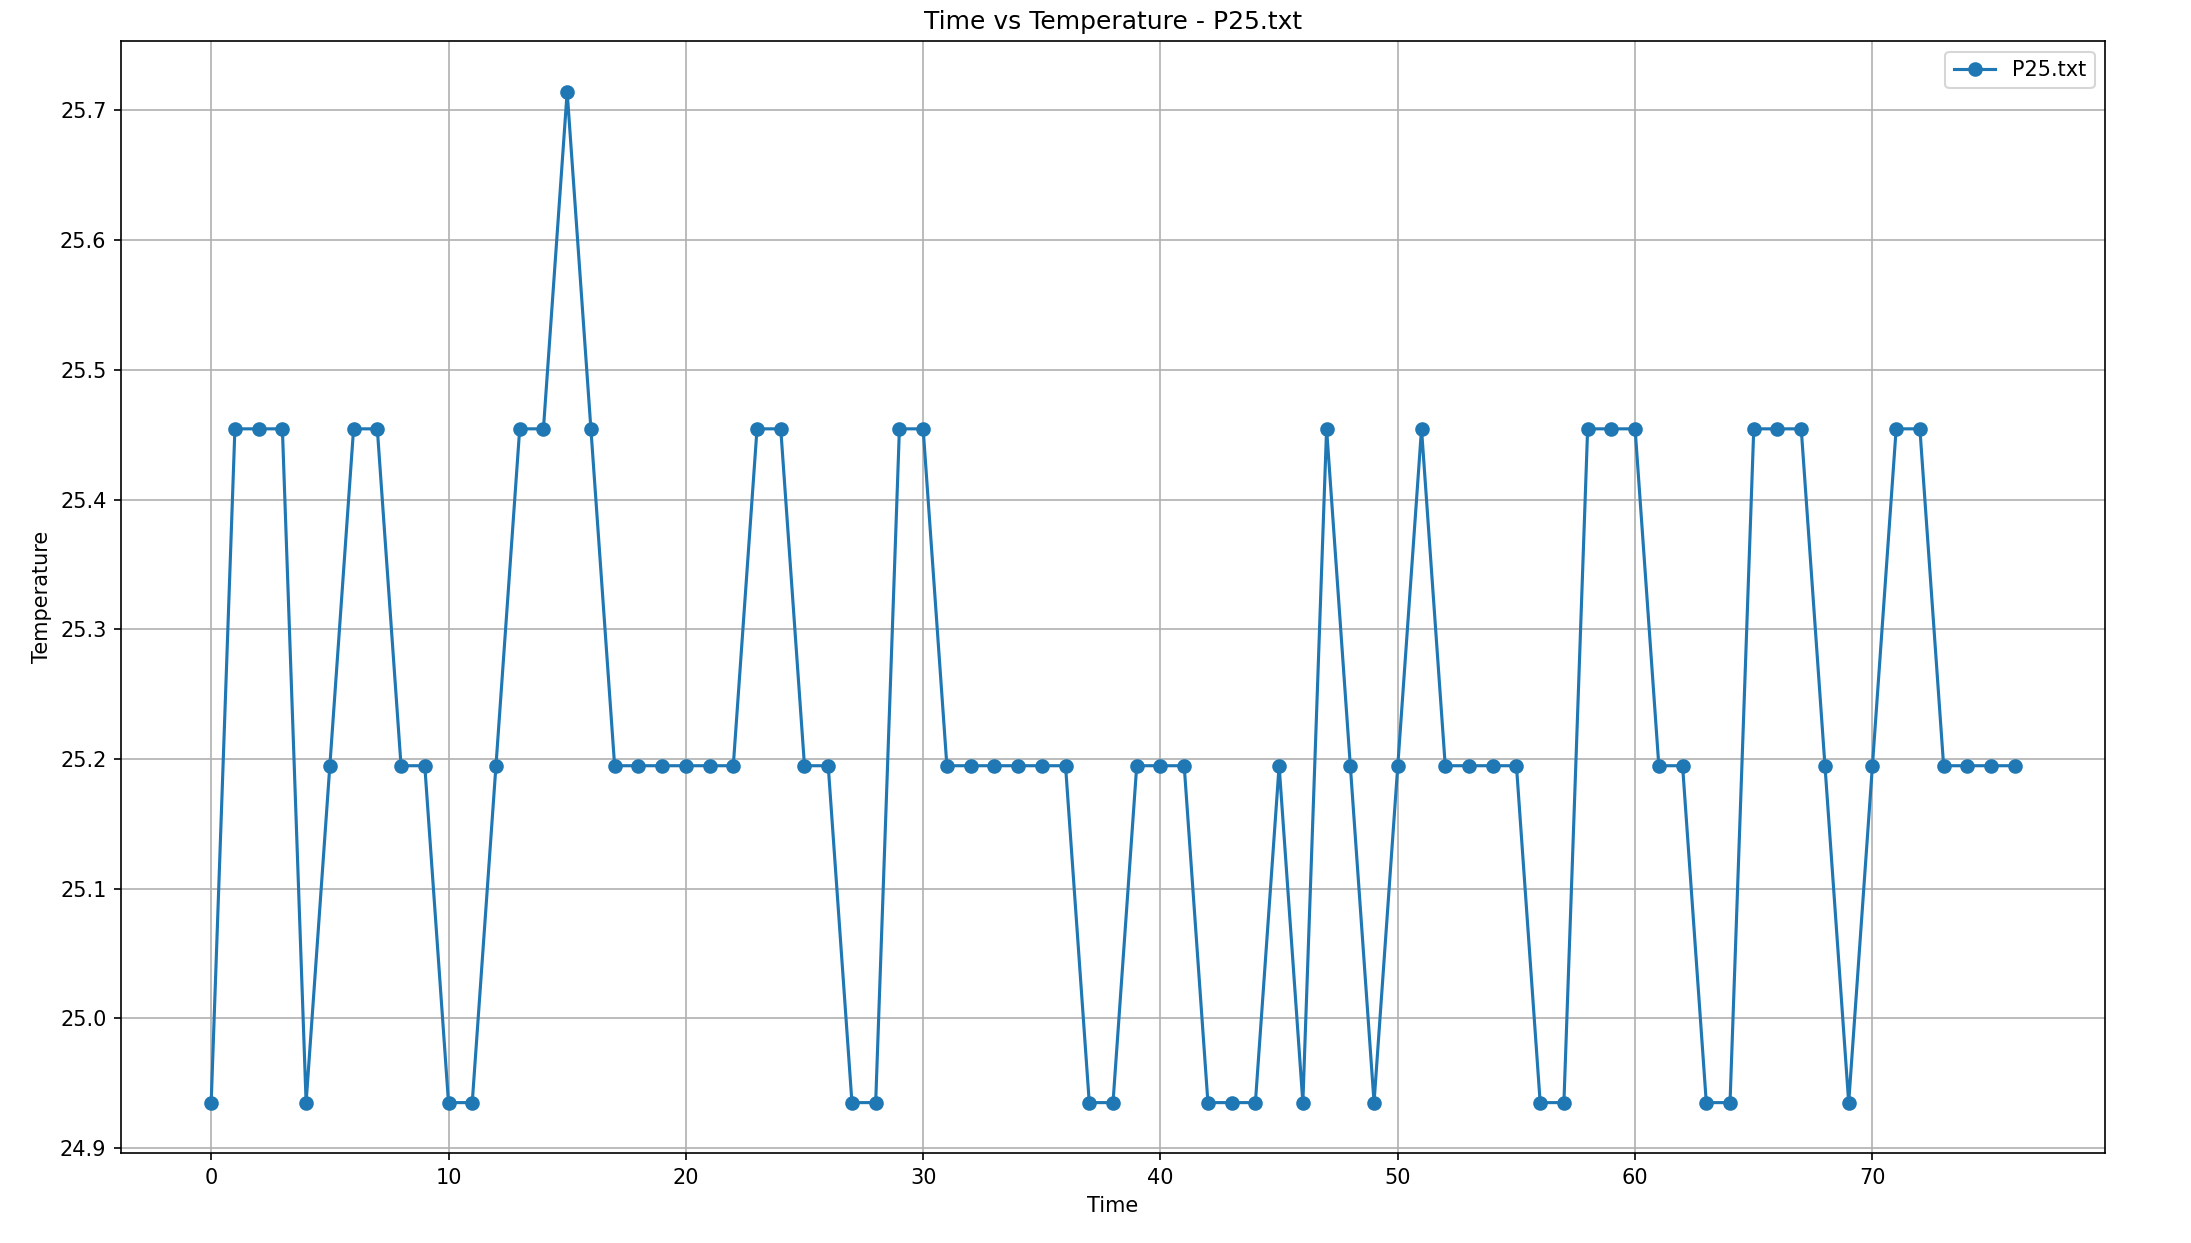
\includegraphics[width=0.6\linewidth]{P25.png}
		\caption{25℃P控温}
		\label{}
	\end{figure}
	\begin{figure}[{H}]
		\centering
		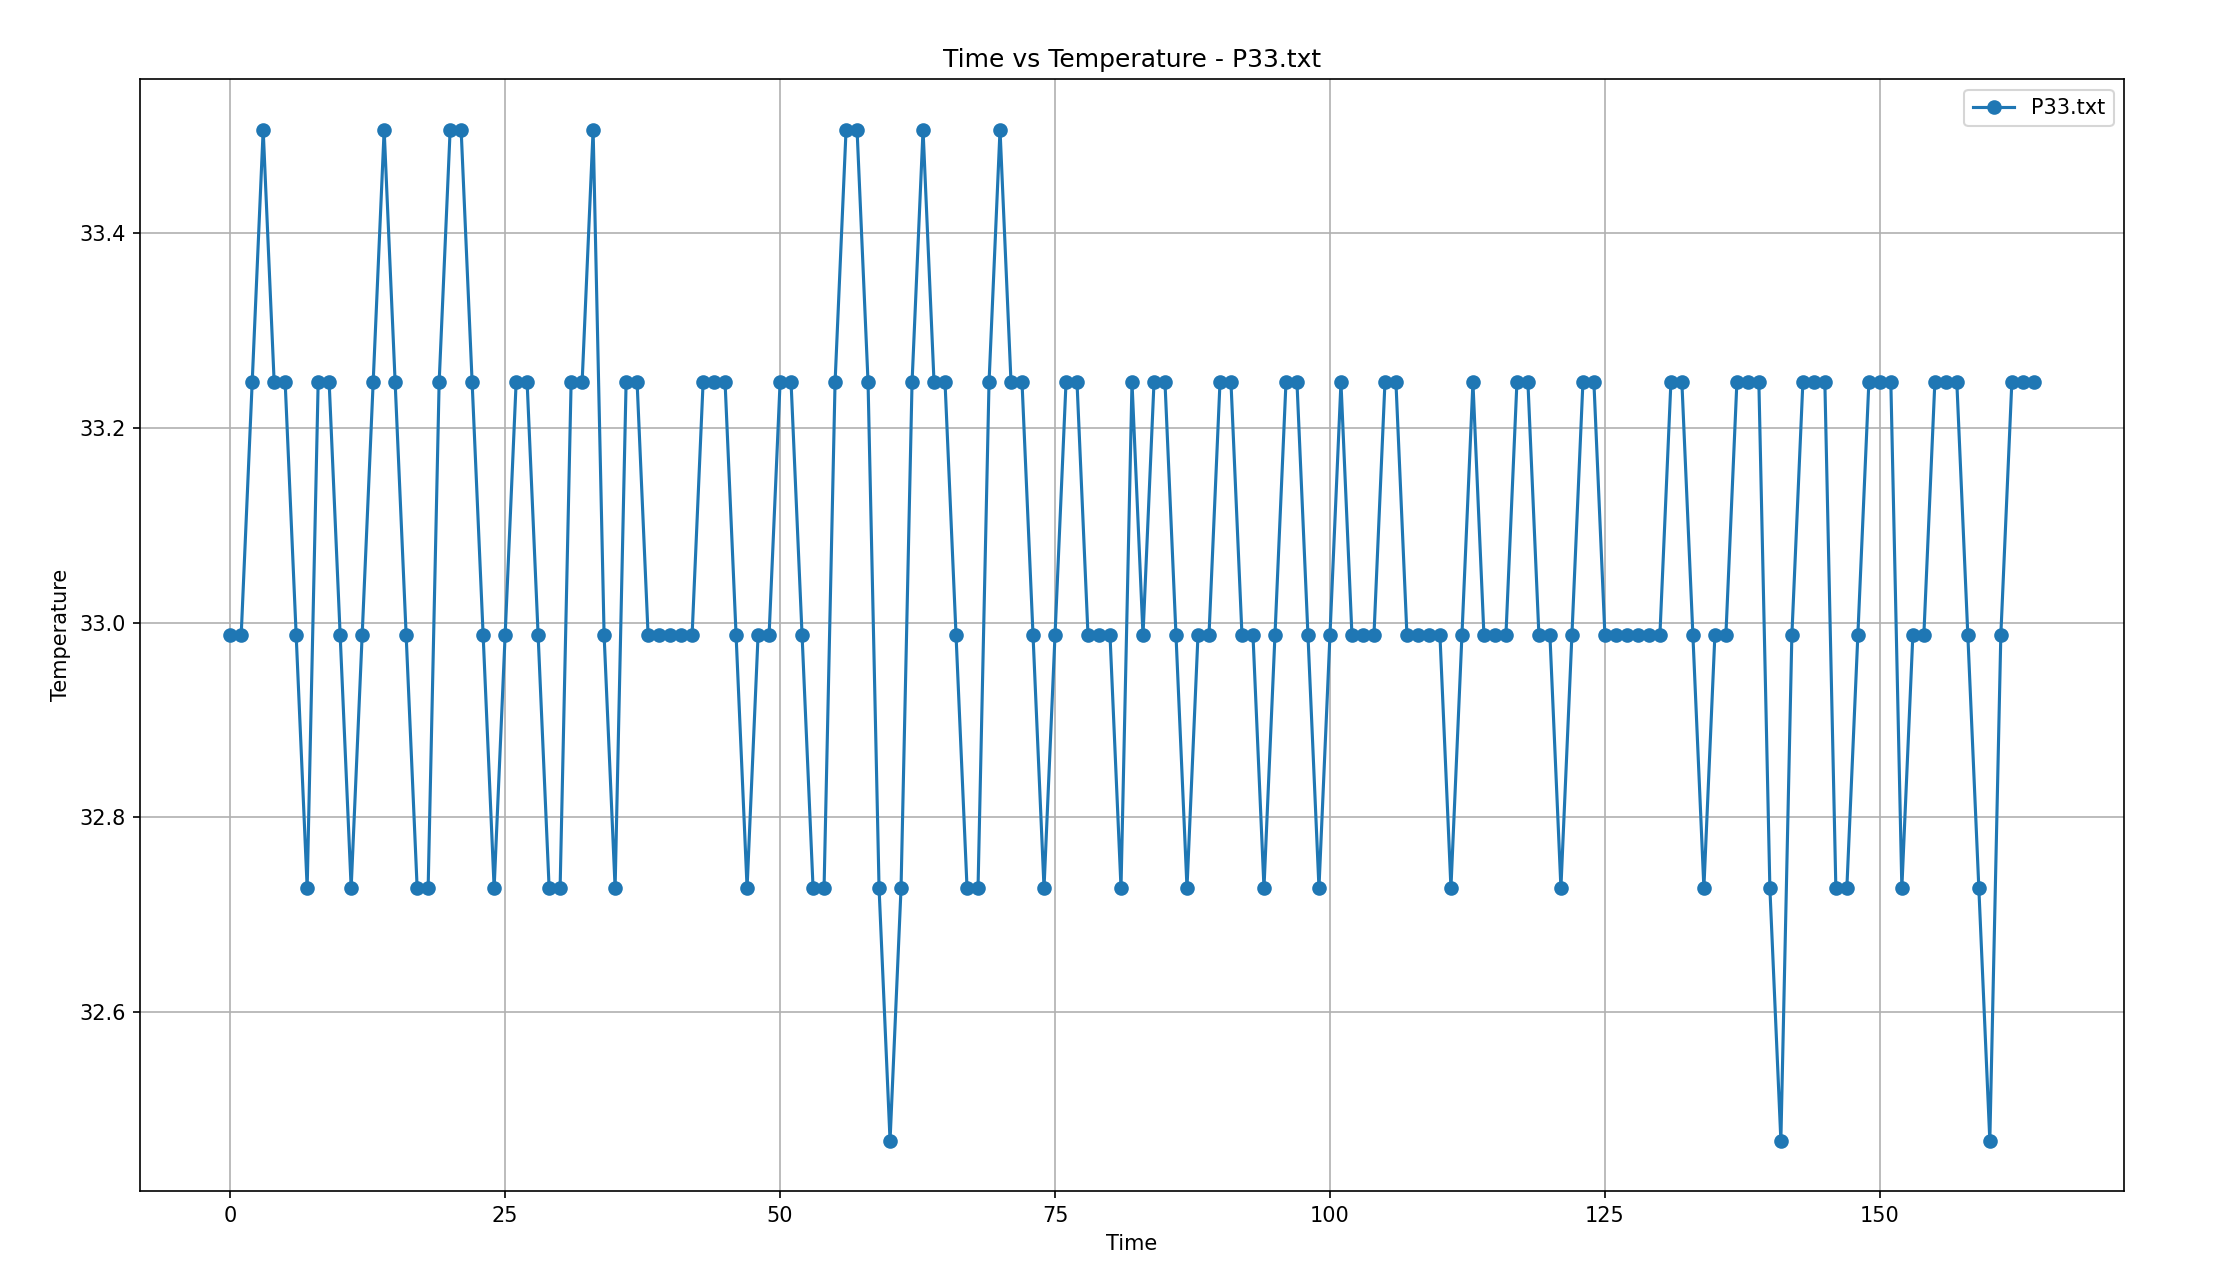
\includegraphics[width=0.6\linewidth]{P33.png}
		\caption{33℃P控温}
		\label{}
	\end{figure}
	\begin{figure}[{H}]
		\centering
		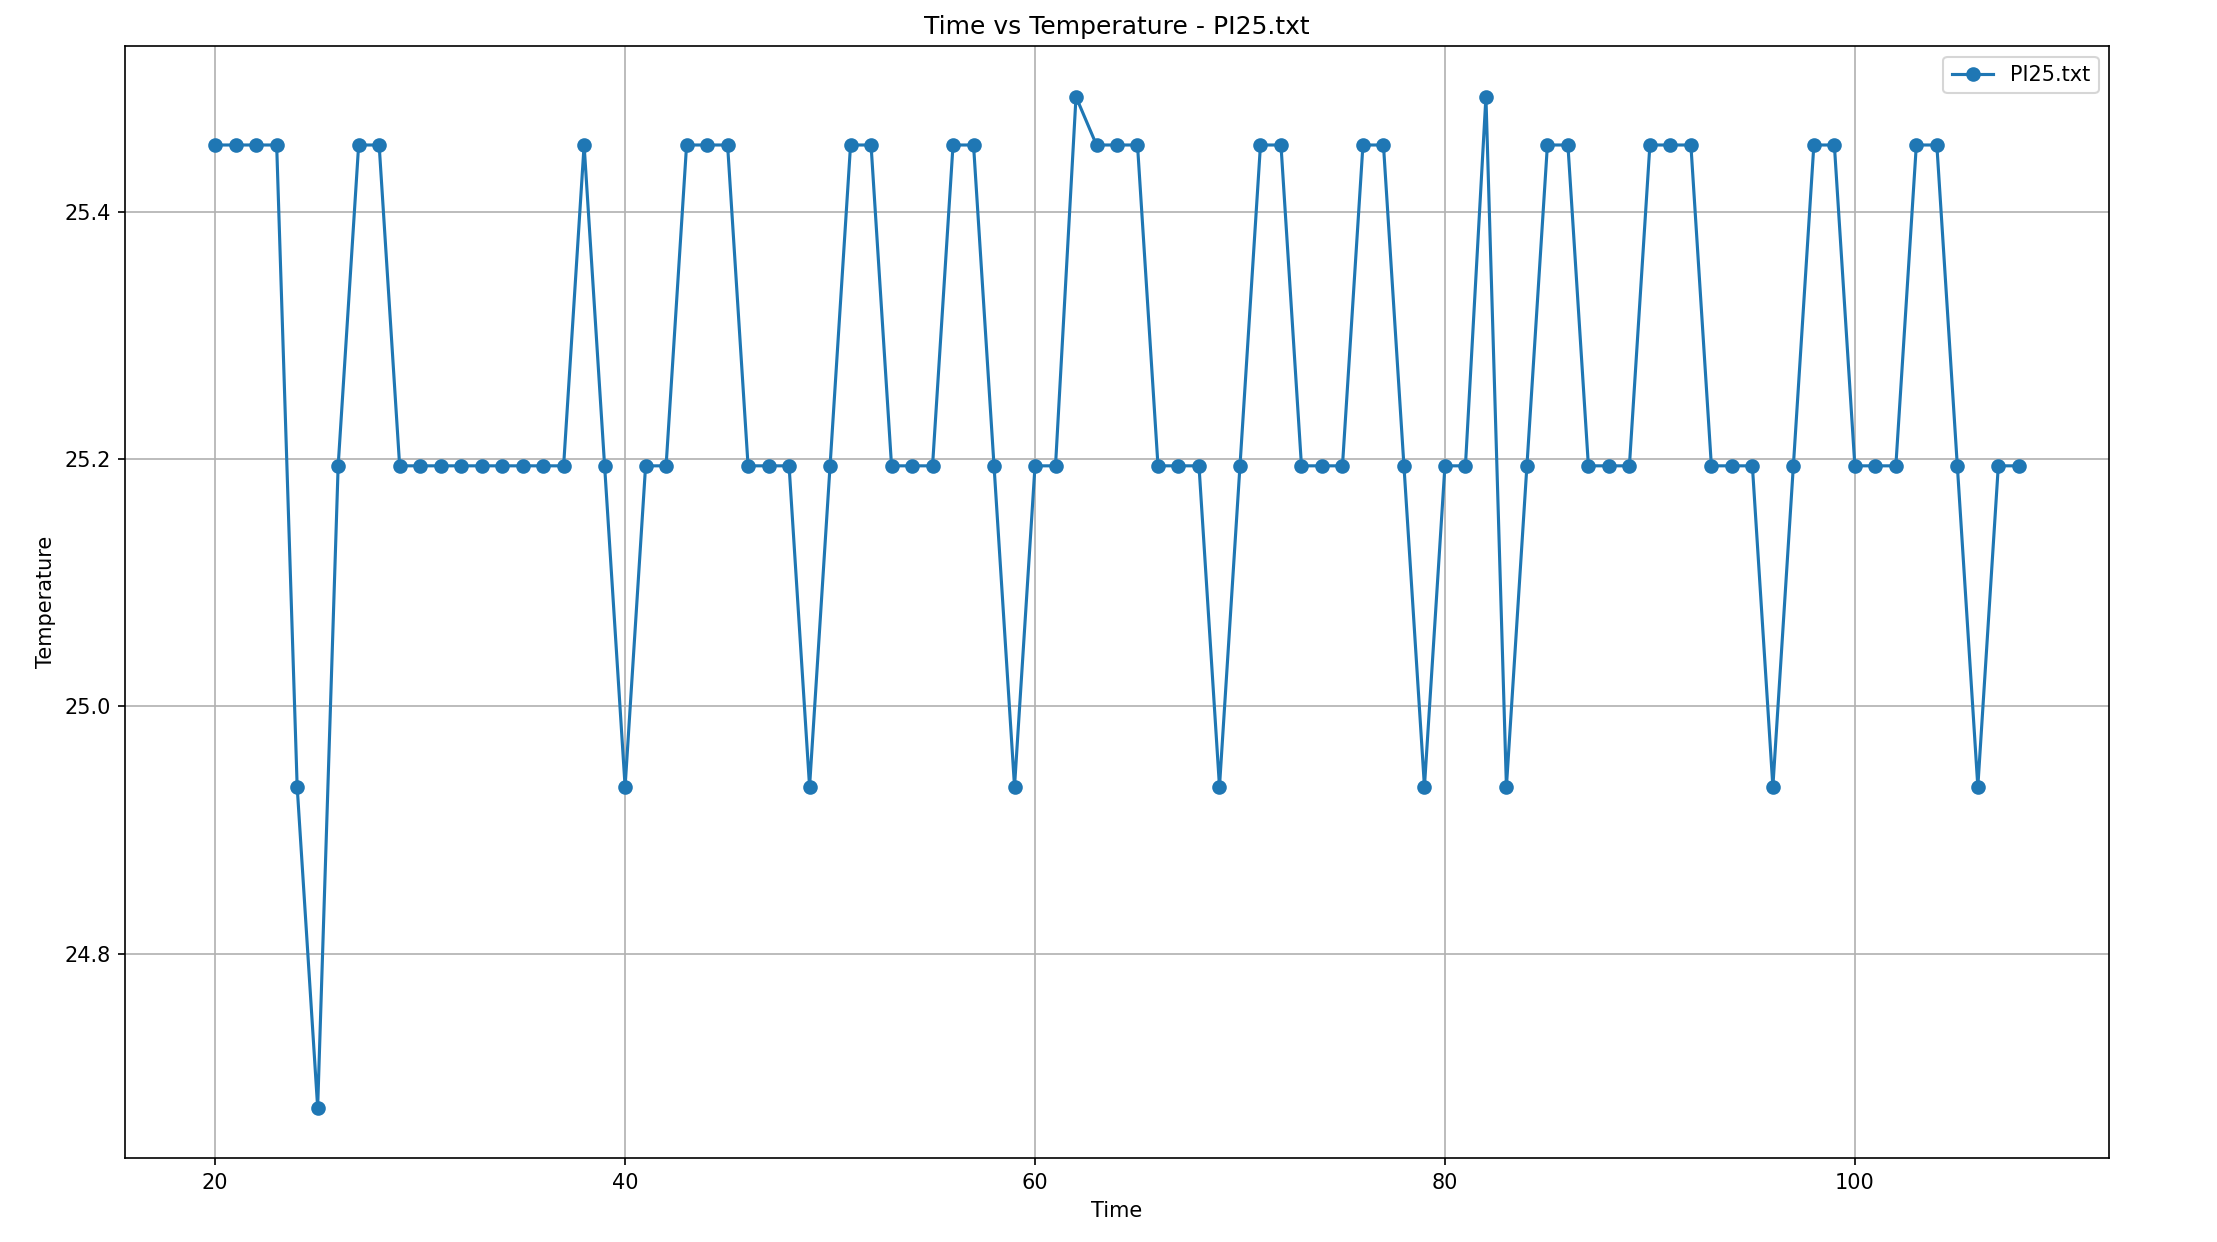
\includegraphics[width=0.6\linewidth]{PI25.png}
		\caption{25℃PI控温}
		\label{}
	\end{figure}
	\begin{figure}[{H}]
		\centering
		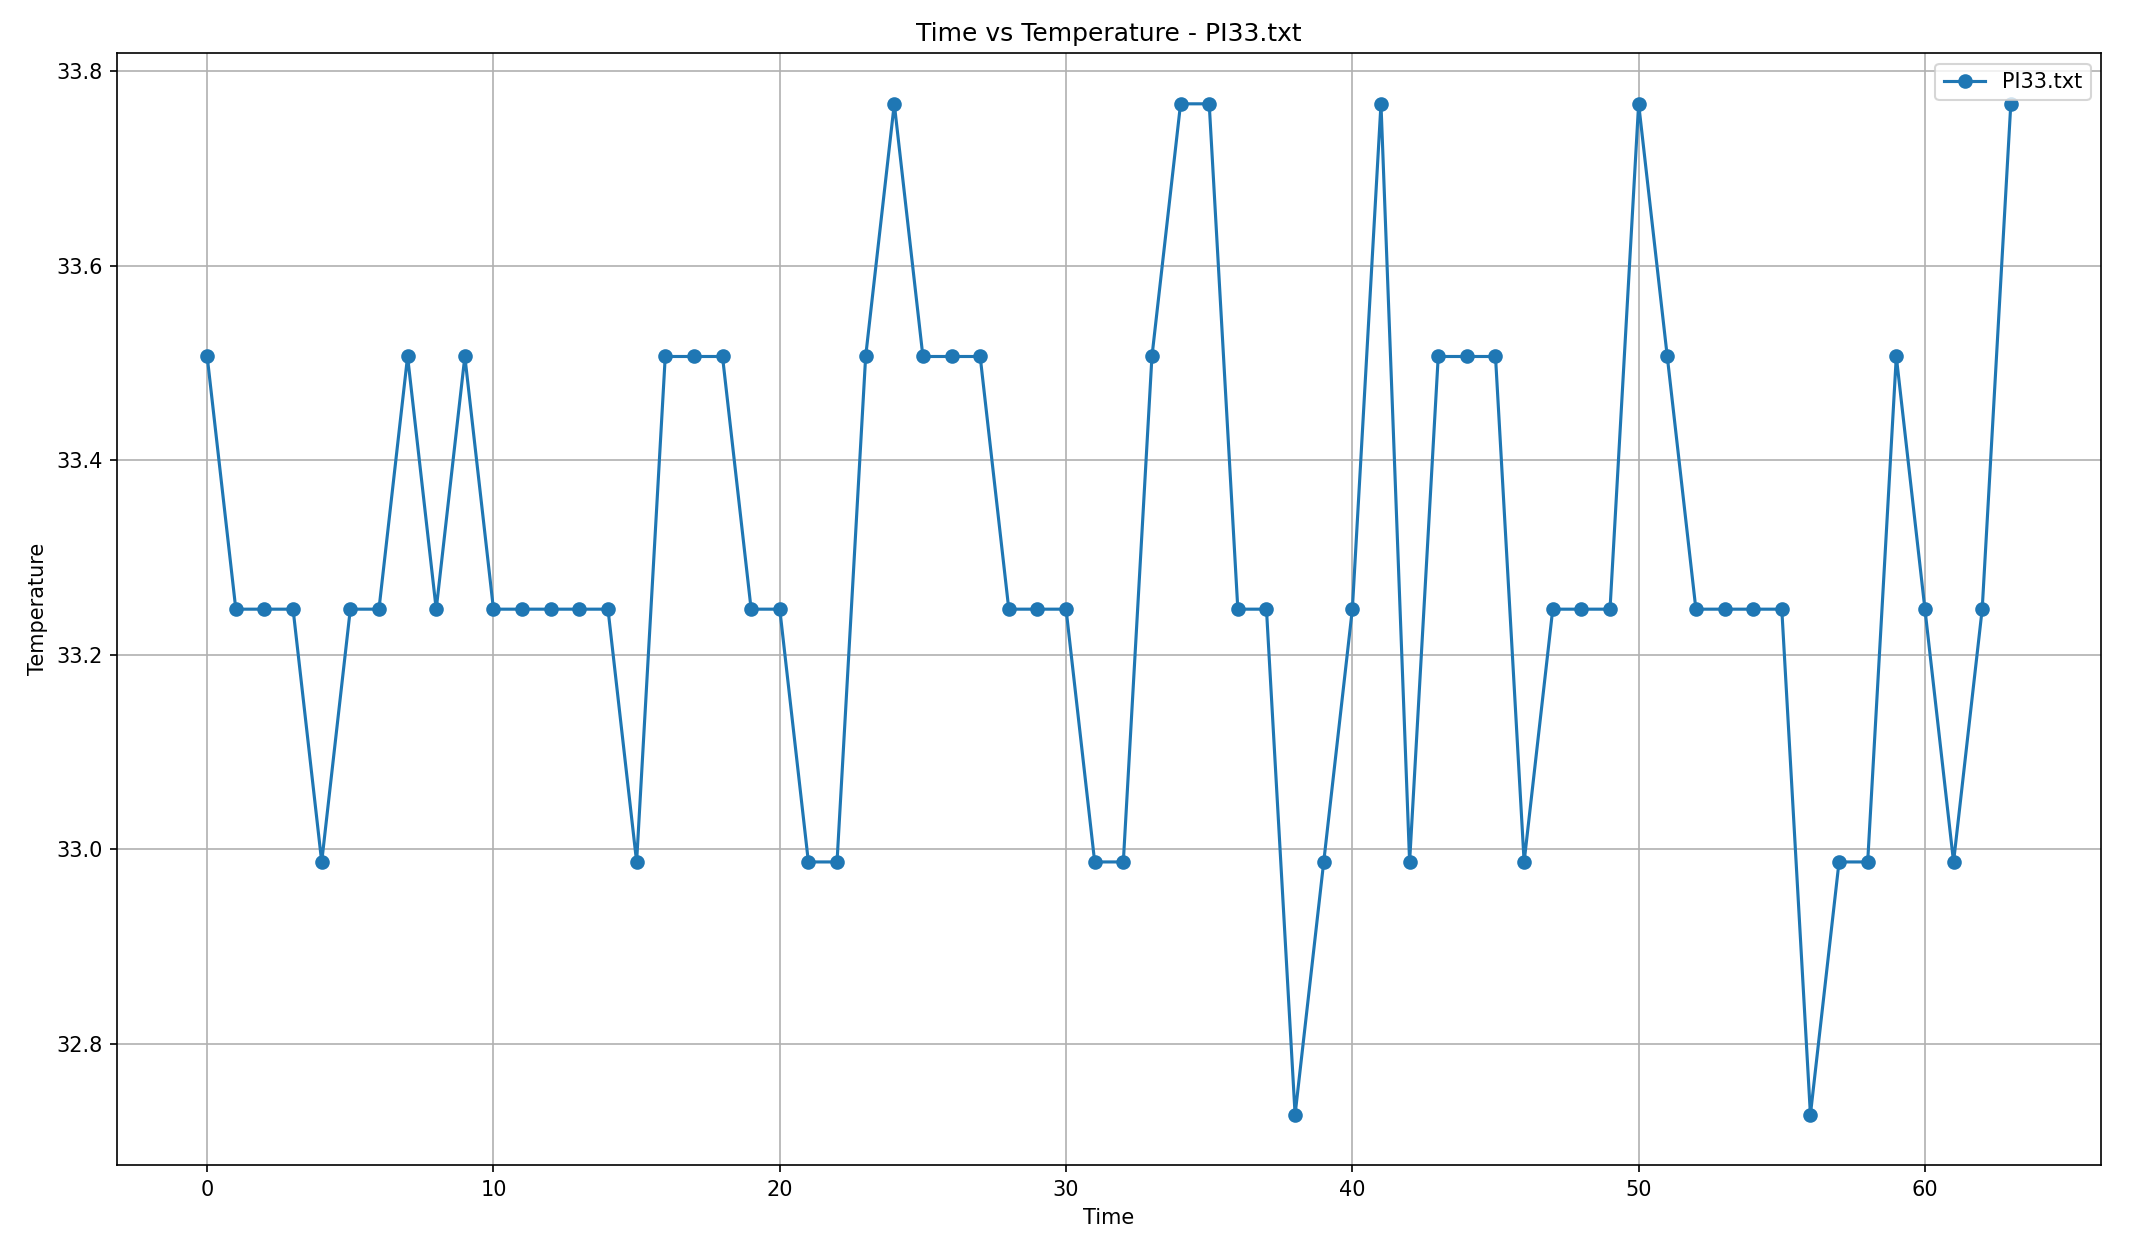
\includegraphics[width=0.6\linewidth]{PI33.png}
		\caption{33℃PI控温}
		\label{}
	\end{figure}
	\begin{figure}[{H}]
		\centering
		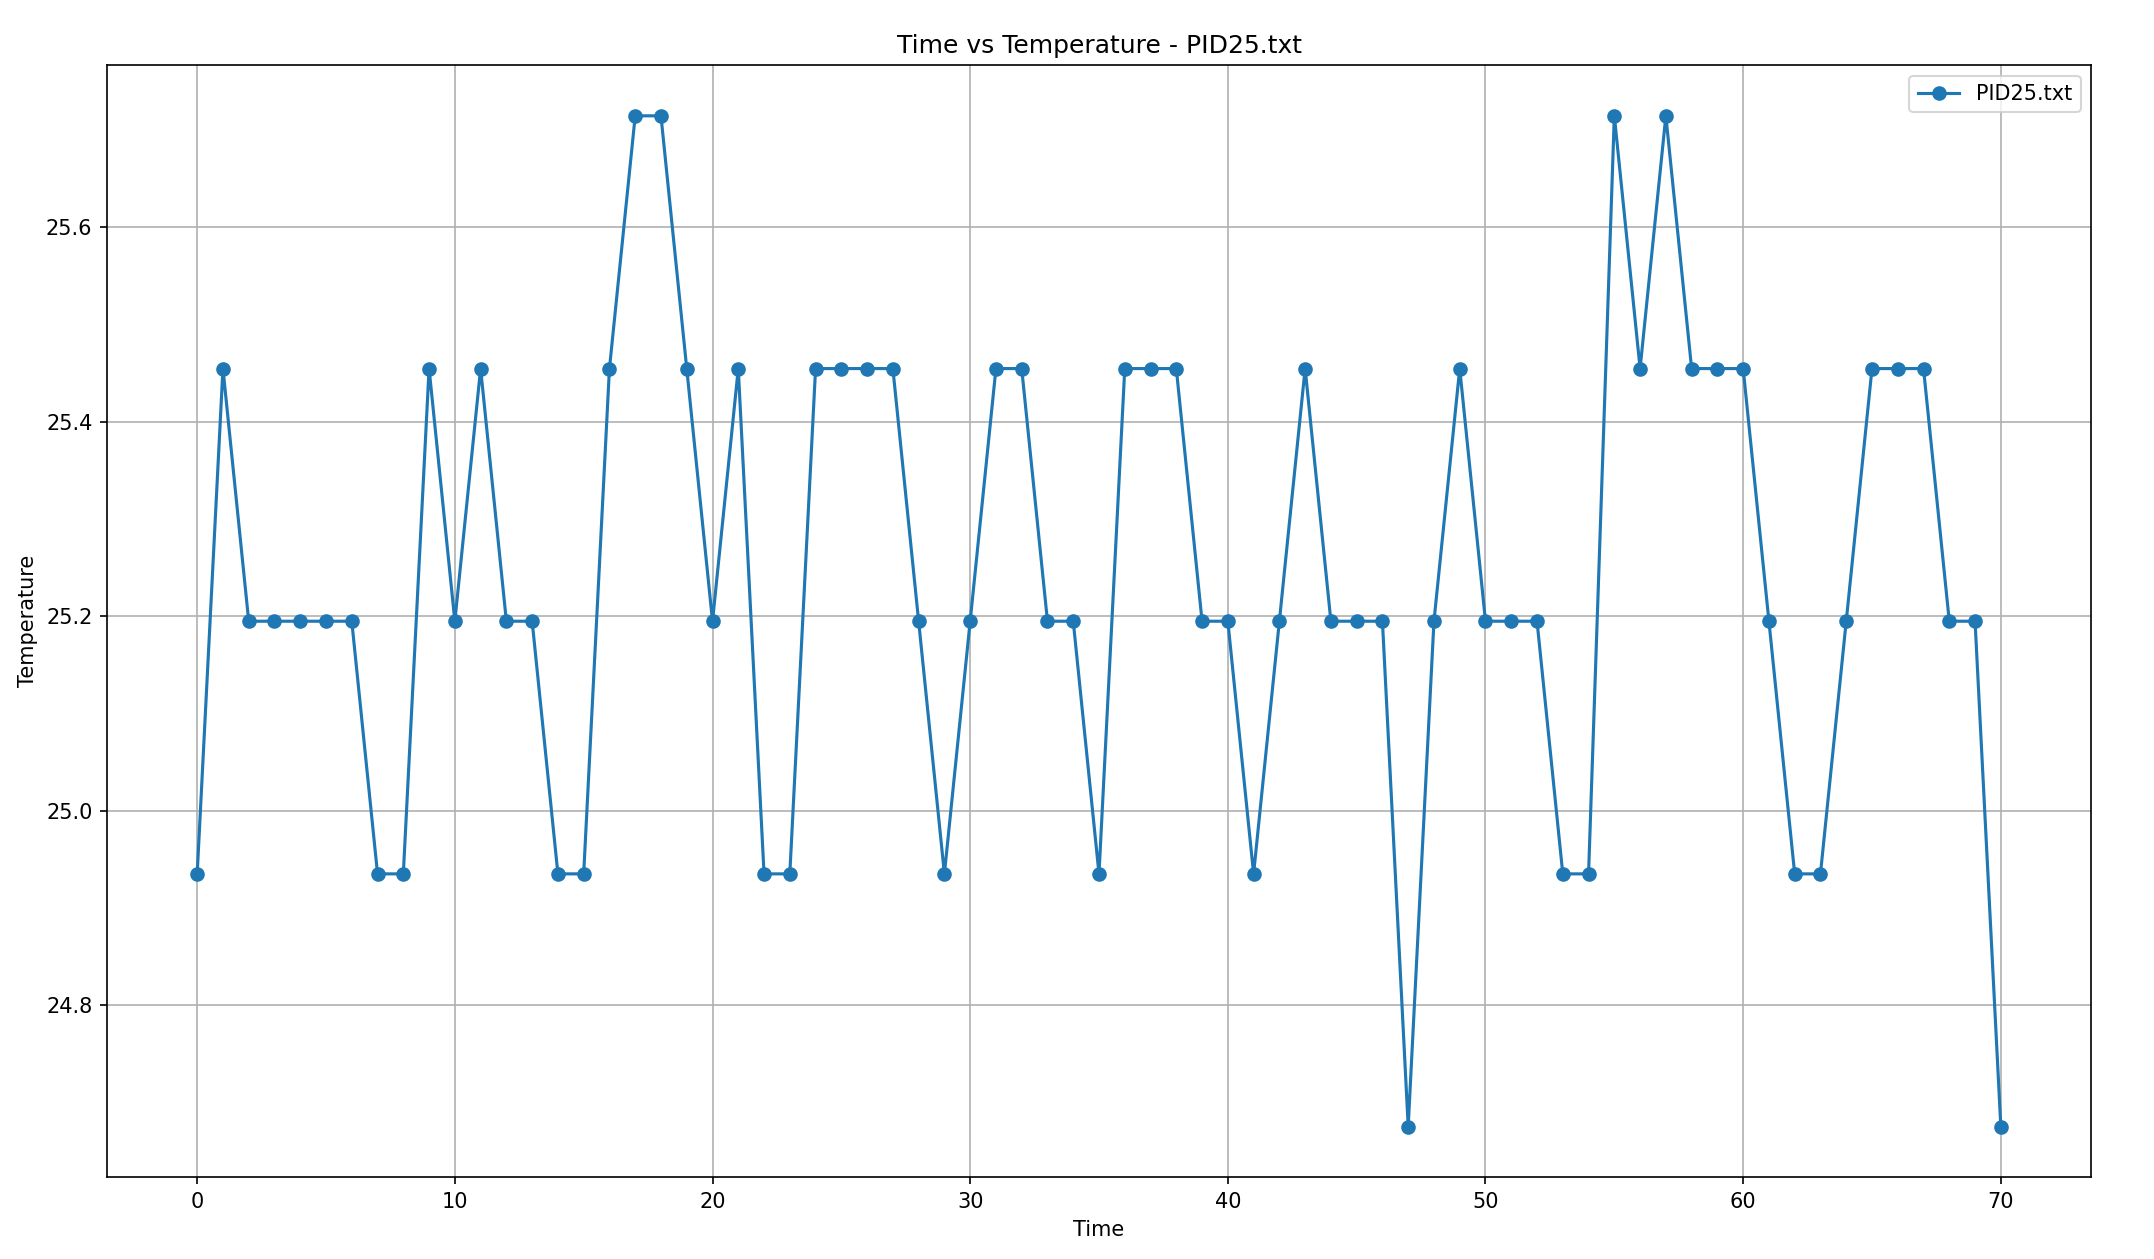
\includegraphics[width=0.6\linewidth]{PID25.png}
		\caption{25℃PID控温}
		\label{}
	\end{figure}
	\begin{figure}[{H}]
		\centering
		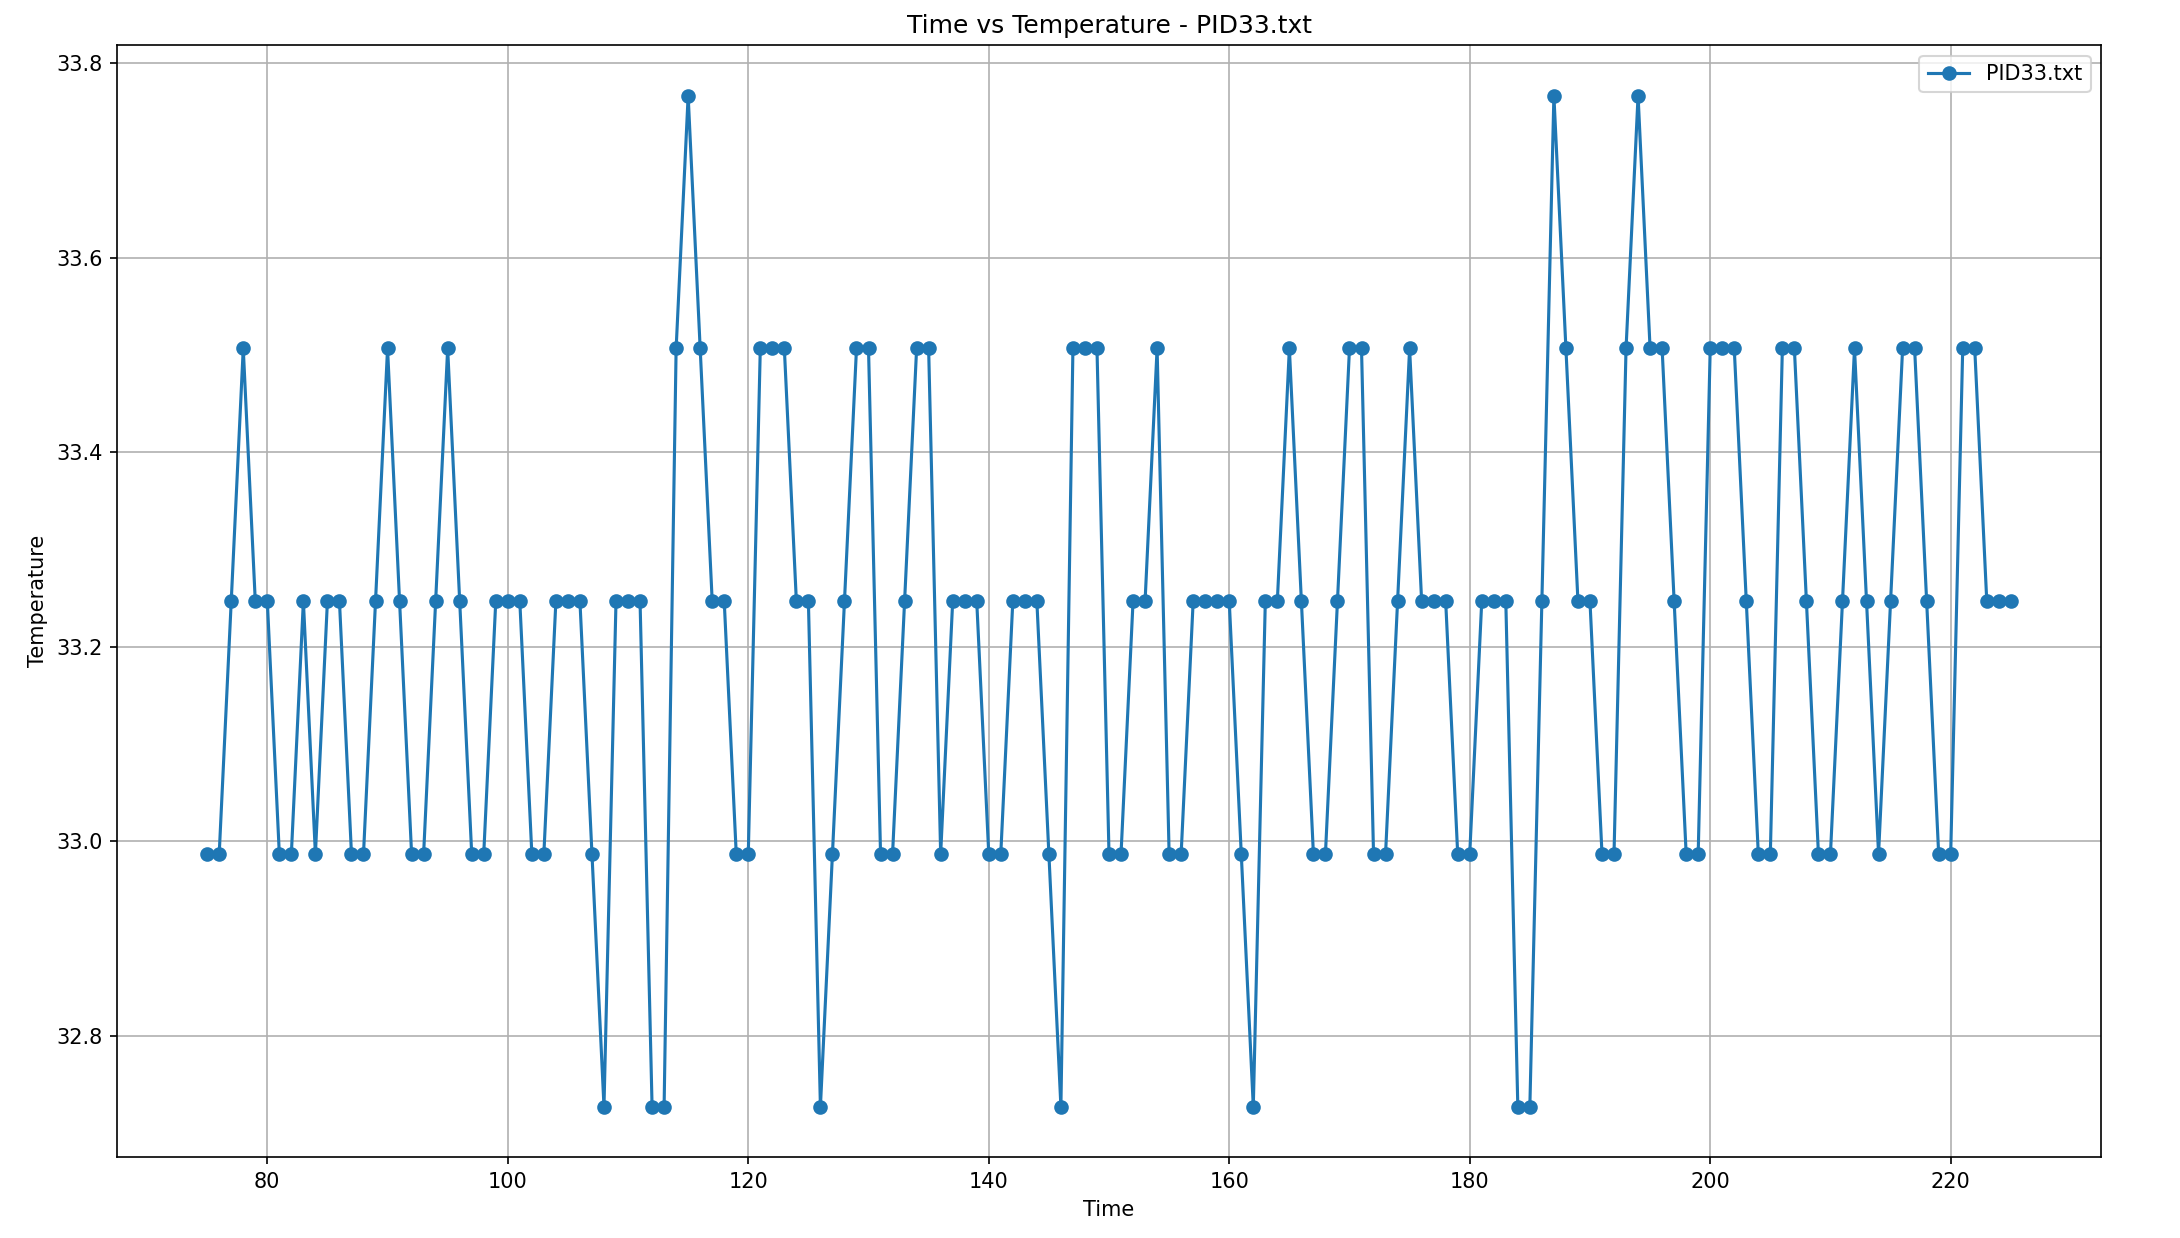
\includegraphics[width=0.7\linewidth]{PID33.png}
		\caption{33℃PID控温}
		\label{}
	\end{figure}
	%
	\subsubsection{数据频域图}
	\begin{figure}[{H}]
		\centering
		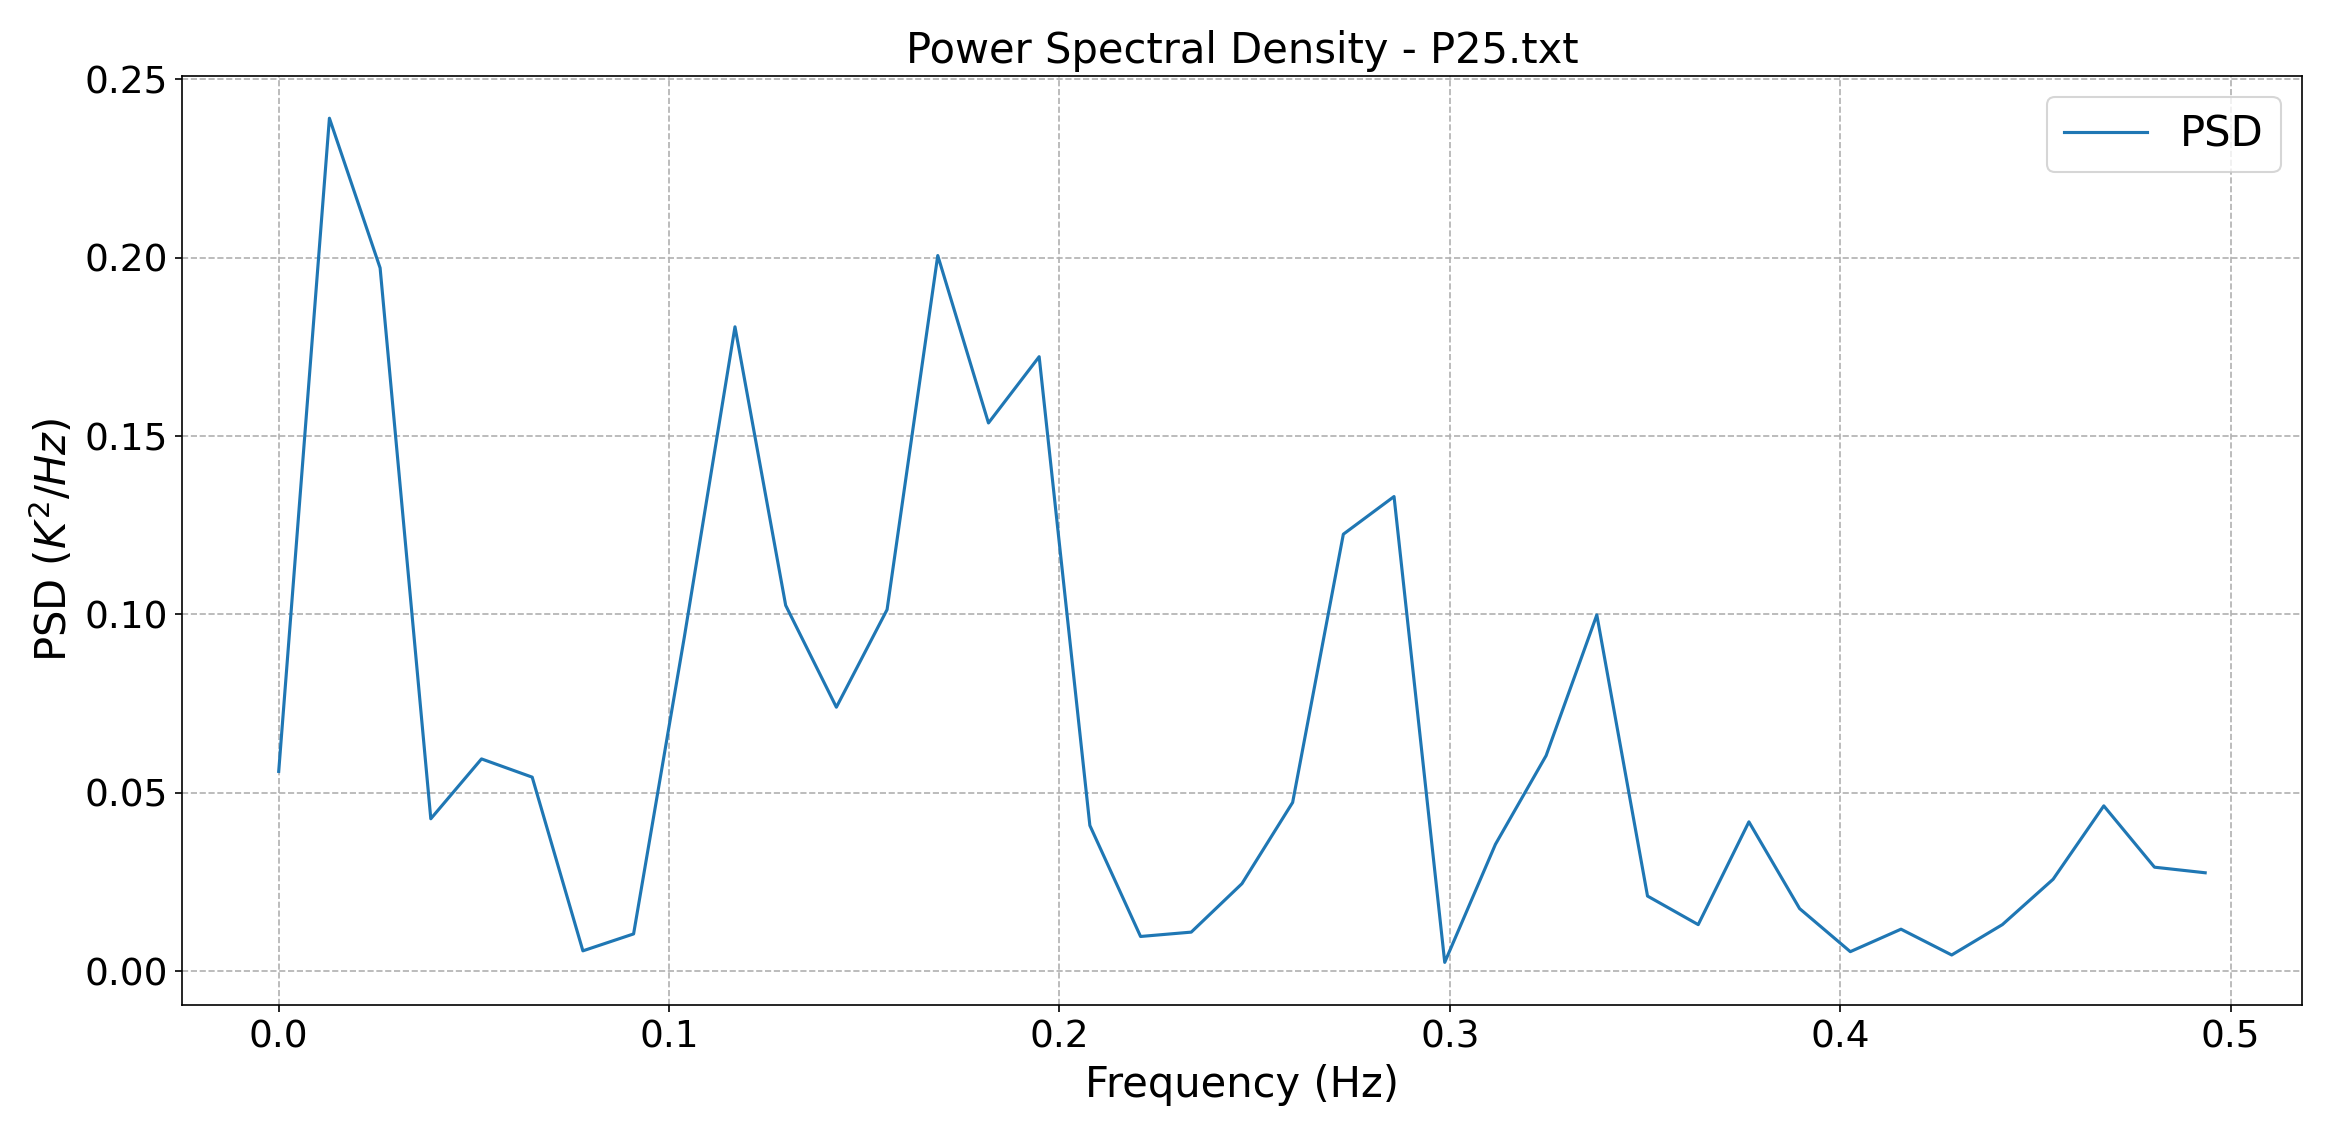
\includegraphics[width=0.6\linewidth]{PSDP25.png}
		\caption{25℃P控温PSD}
		\label{}
	\end{figure}
	\begin{figure}[{H}]
		\centering
		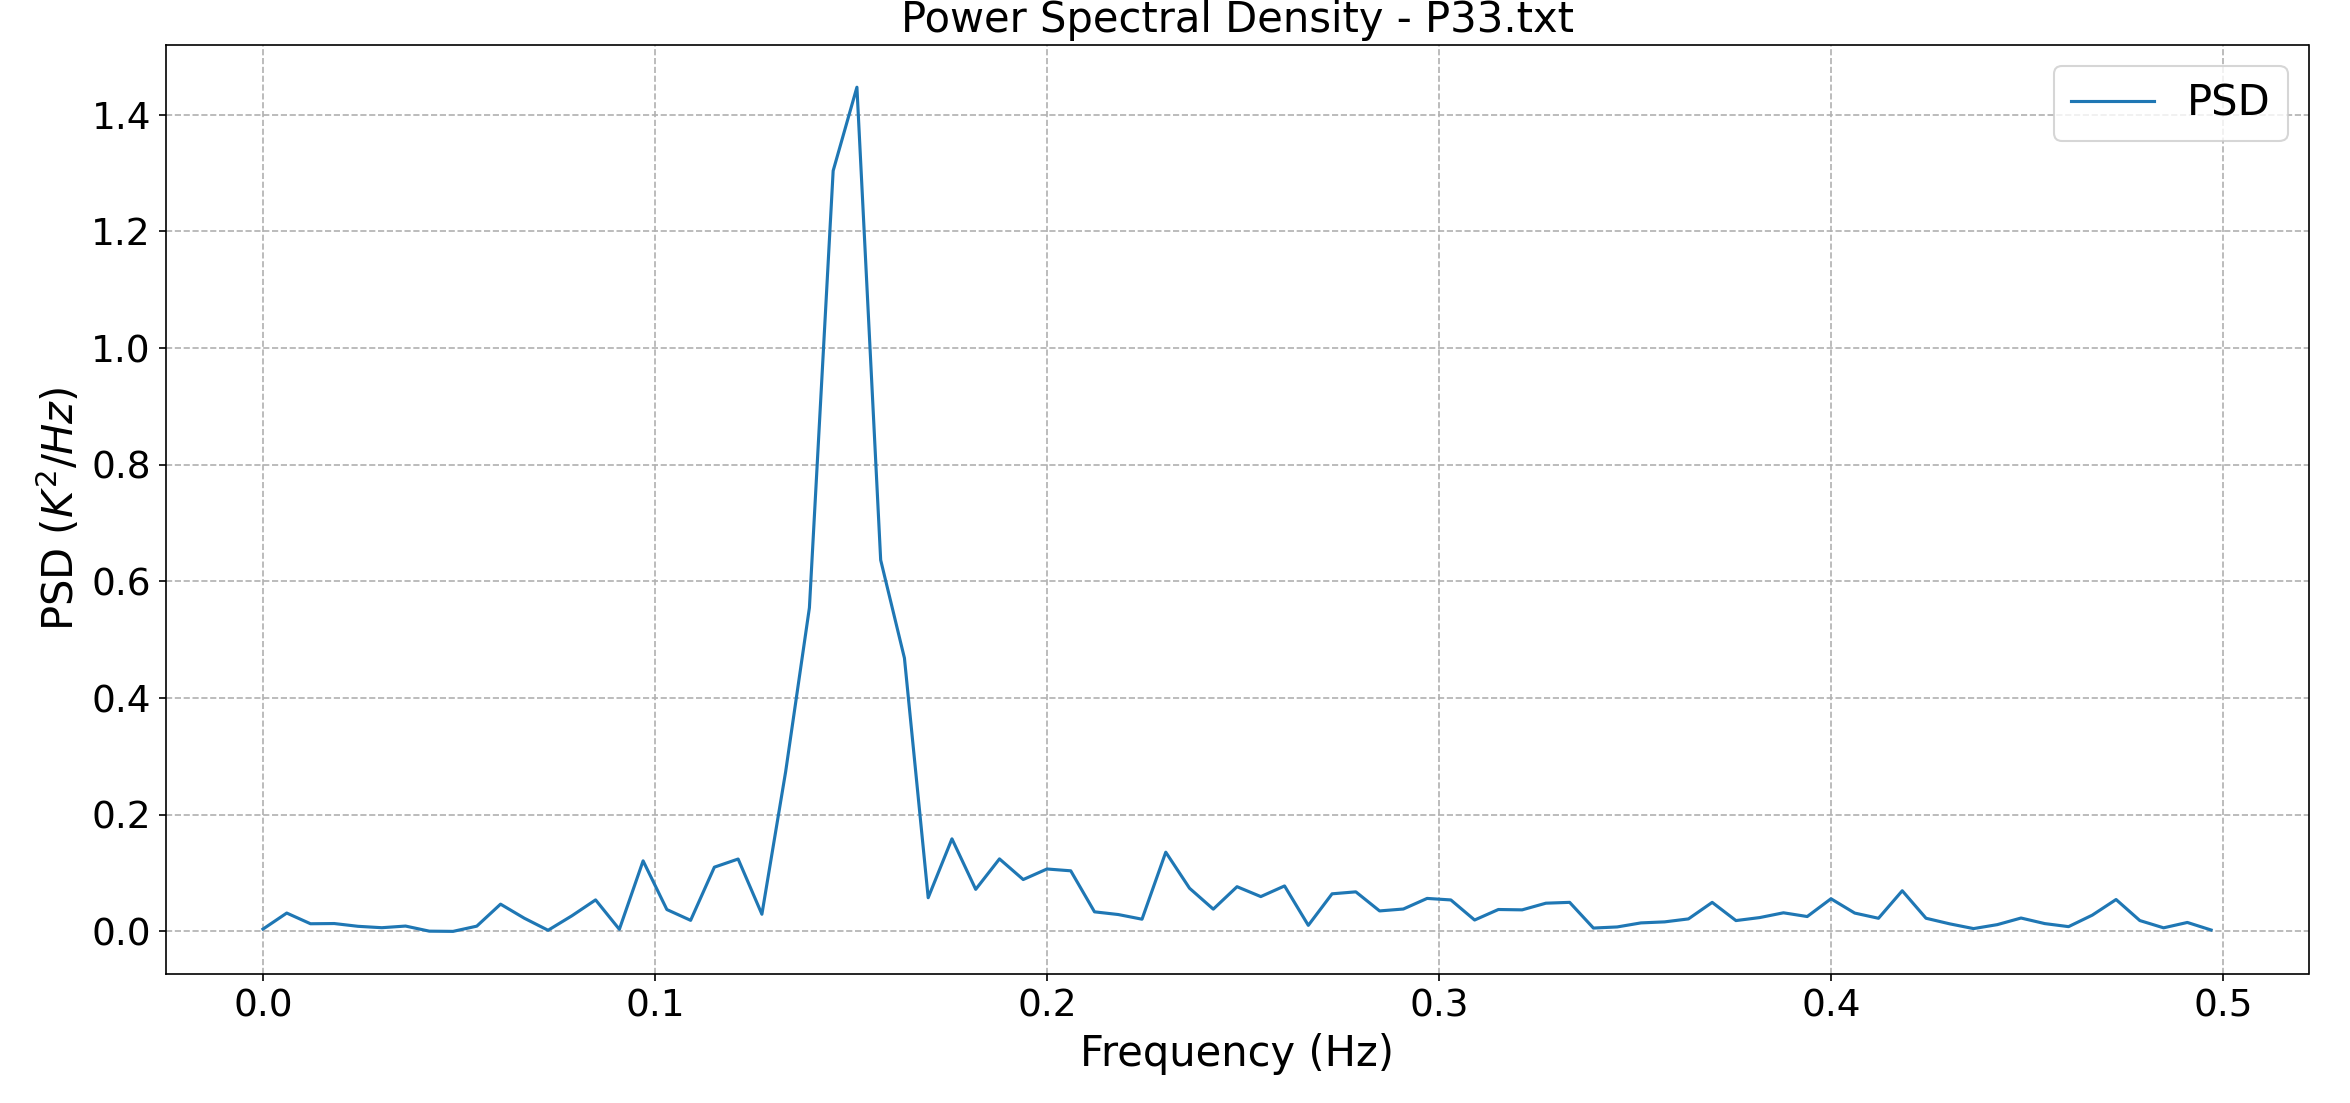
\includegraphics[width=0.6\linewidth]{PSDP33.png}
		\caption{33℃P控温PSD}
		\label{}
	\end{figure}
	\begin{figure}[{H}]
		\centering
		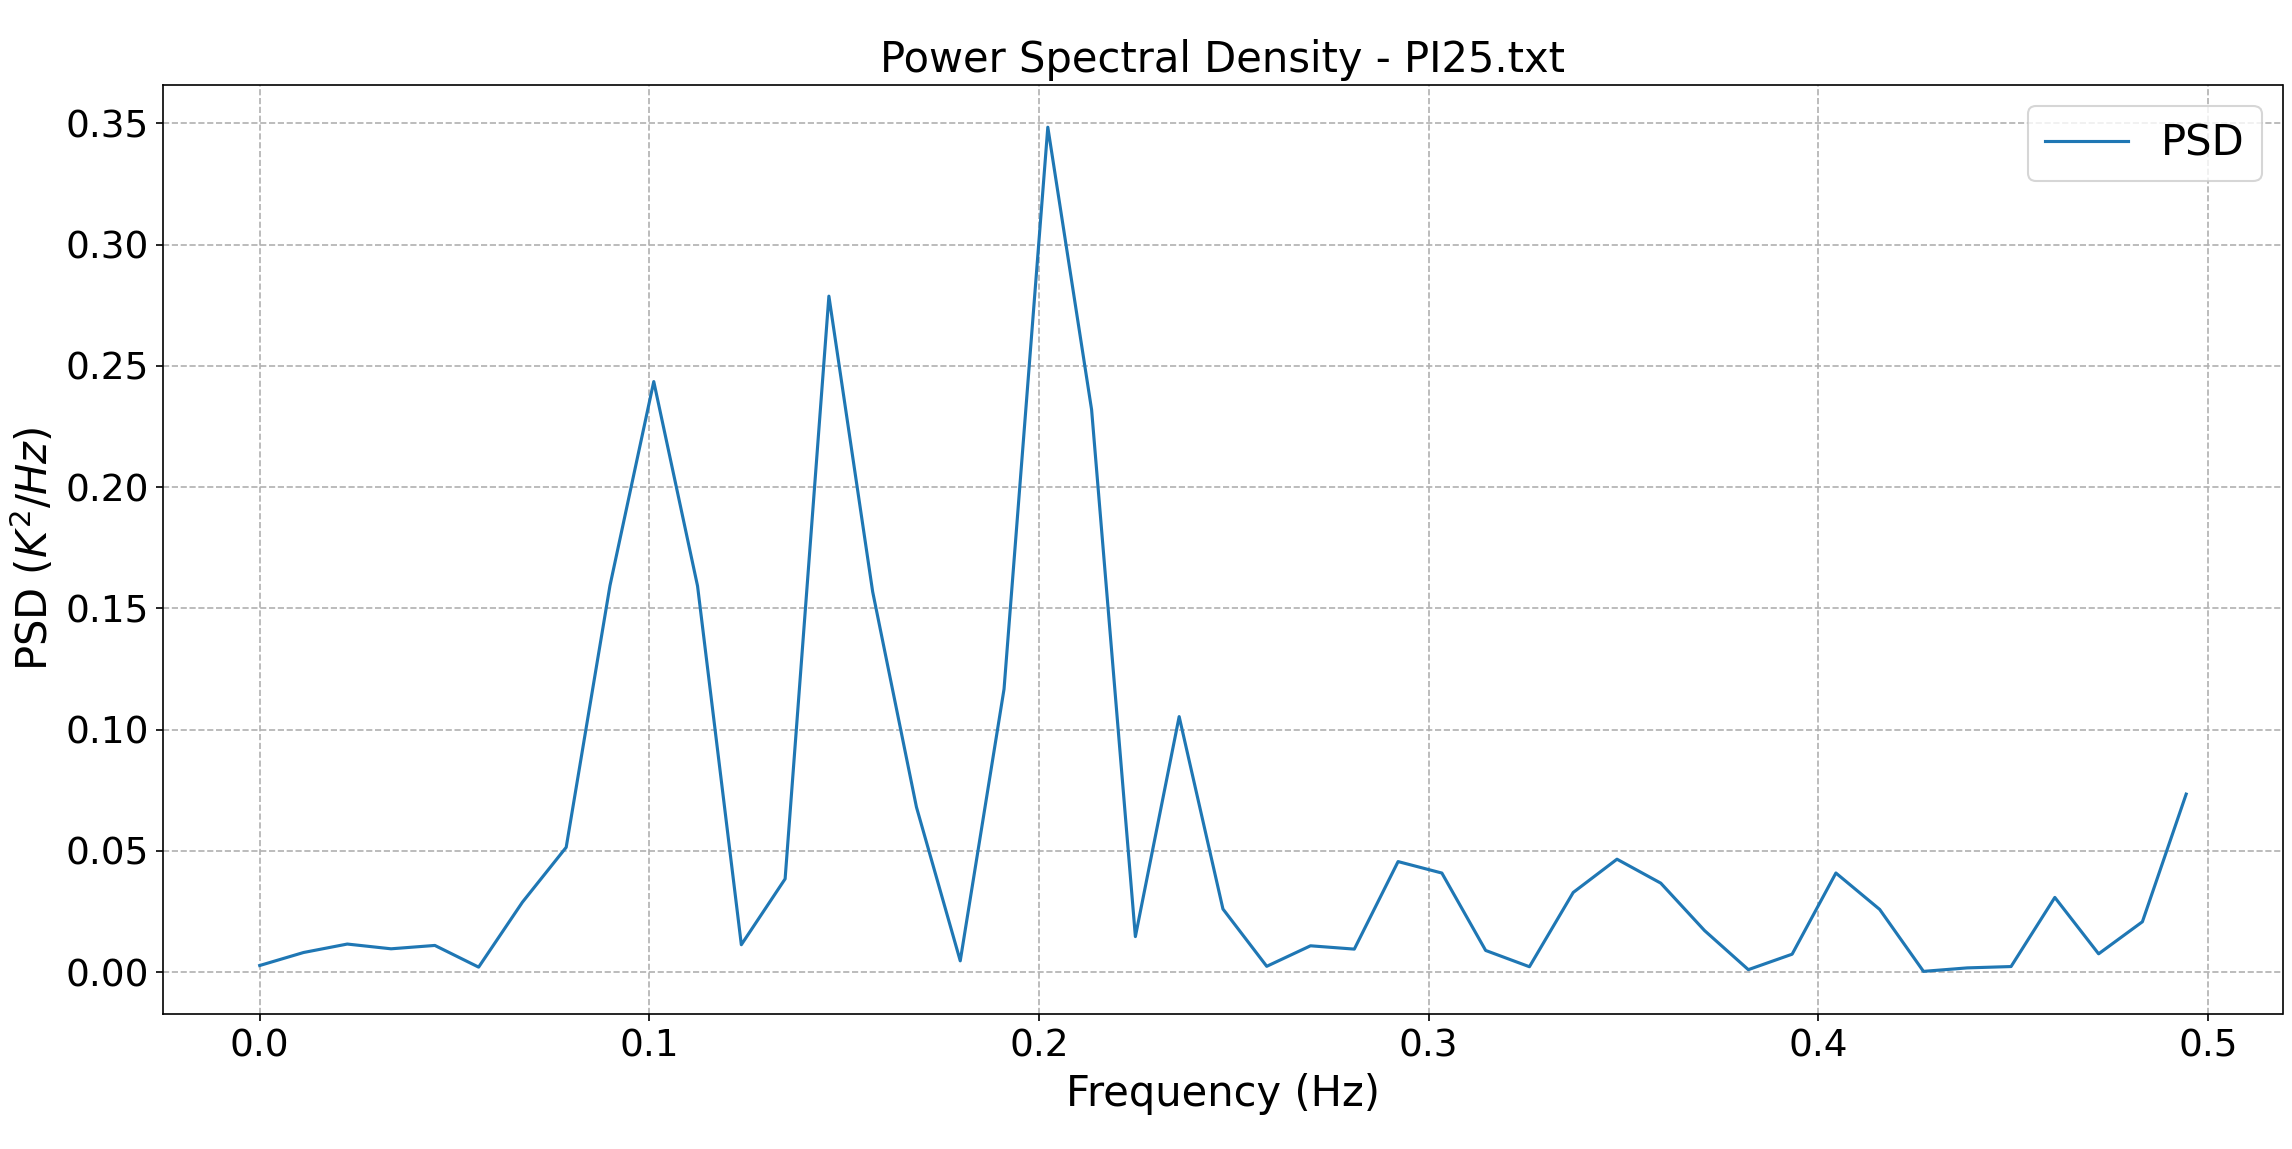
\includegraphics[width=0.6\linewidth]{PSDPI25.png}
		\caption{25℃PI控温PSD}
		\label{}
	\end{figure}
	\begin{figure}[{H}]
		\centering
		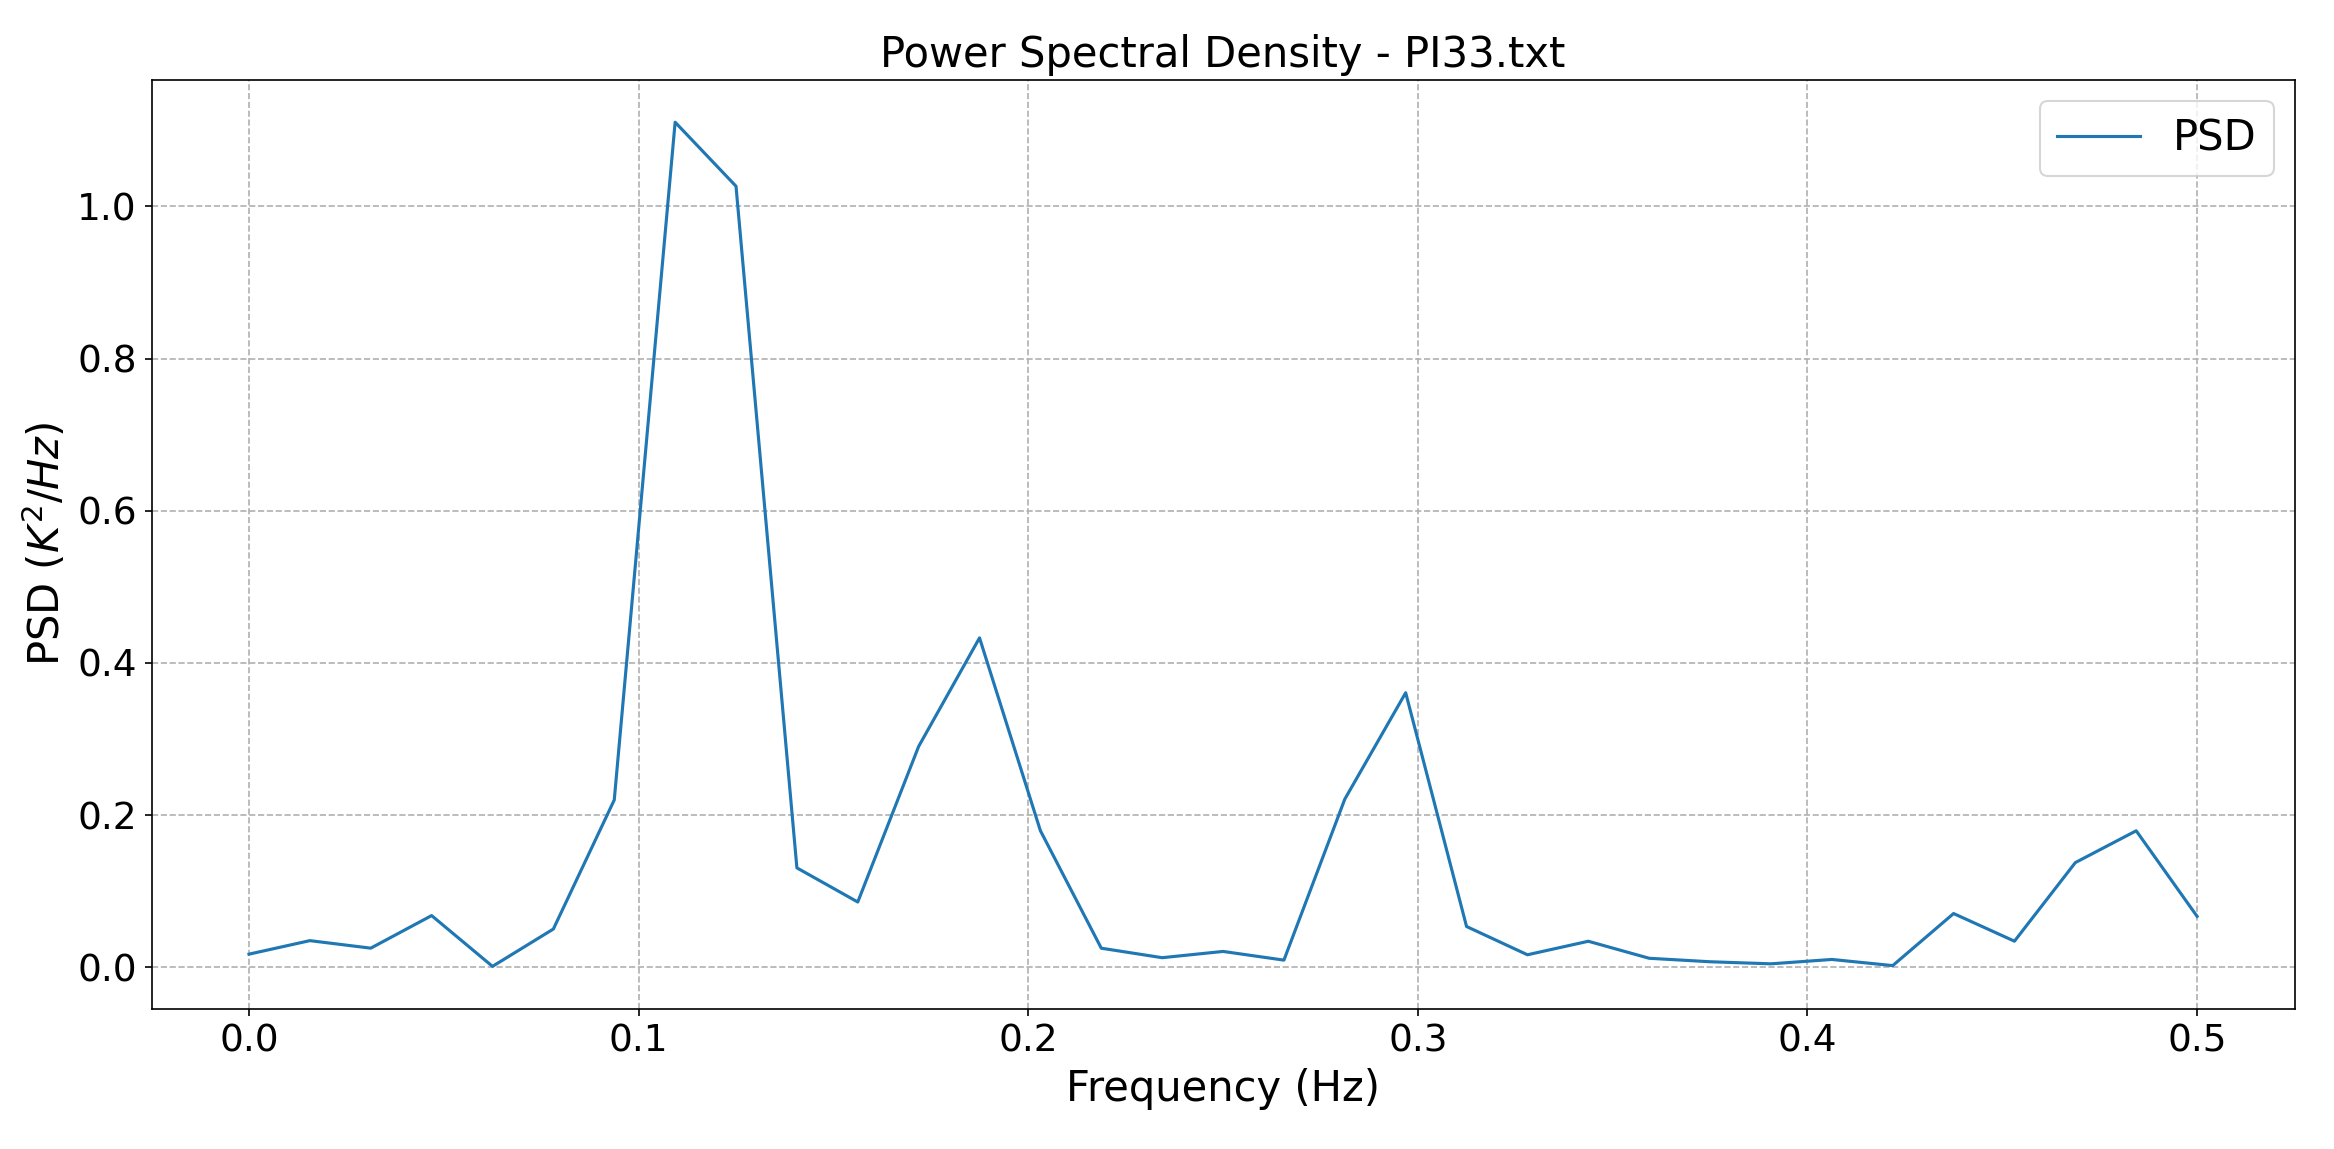
\includegraphics[width=0.6\linewidth]{PSDPI33.png}
		\caption{33℃PI控温PSD}
		\label{}
	\end{figure}
	\begin{figure}[{H}]
		\centering
		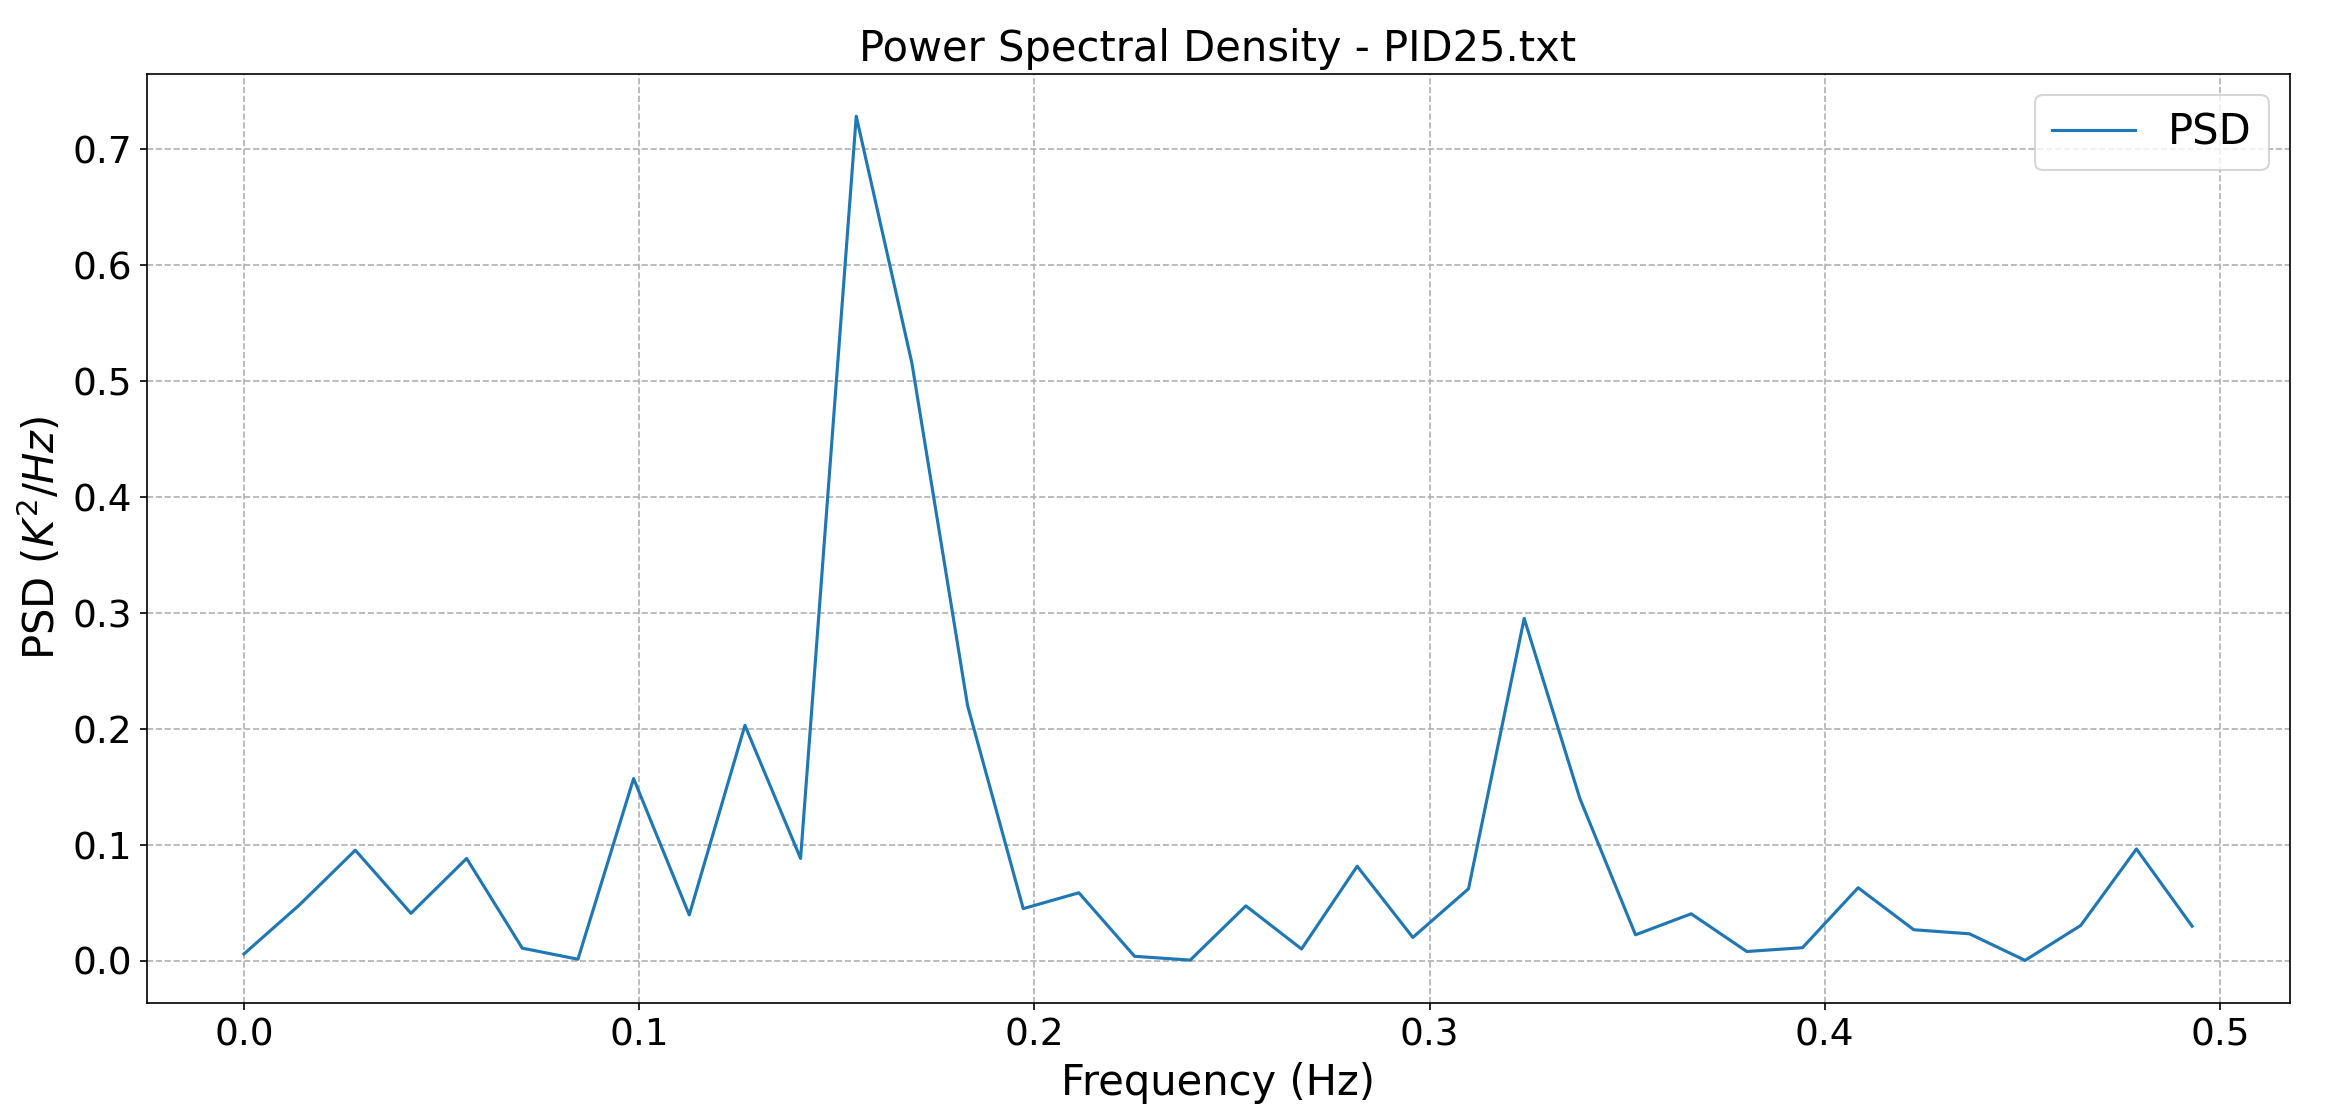
\includegraphics[width=0.6\linewidth]{PSDPID25.png}
		\caption{25℃PID控温PSD}
		\label{}
	\end{figure}
	\begin{figure}[{H}]
		\centering
		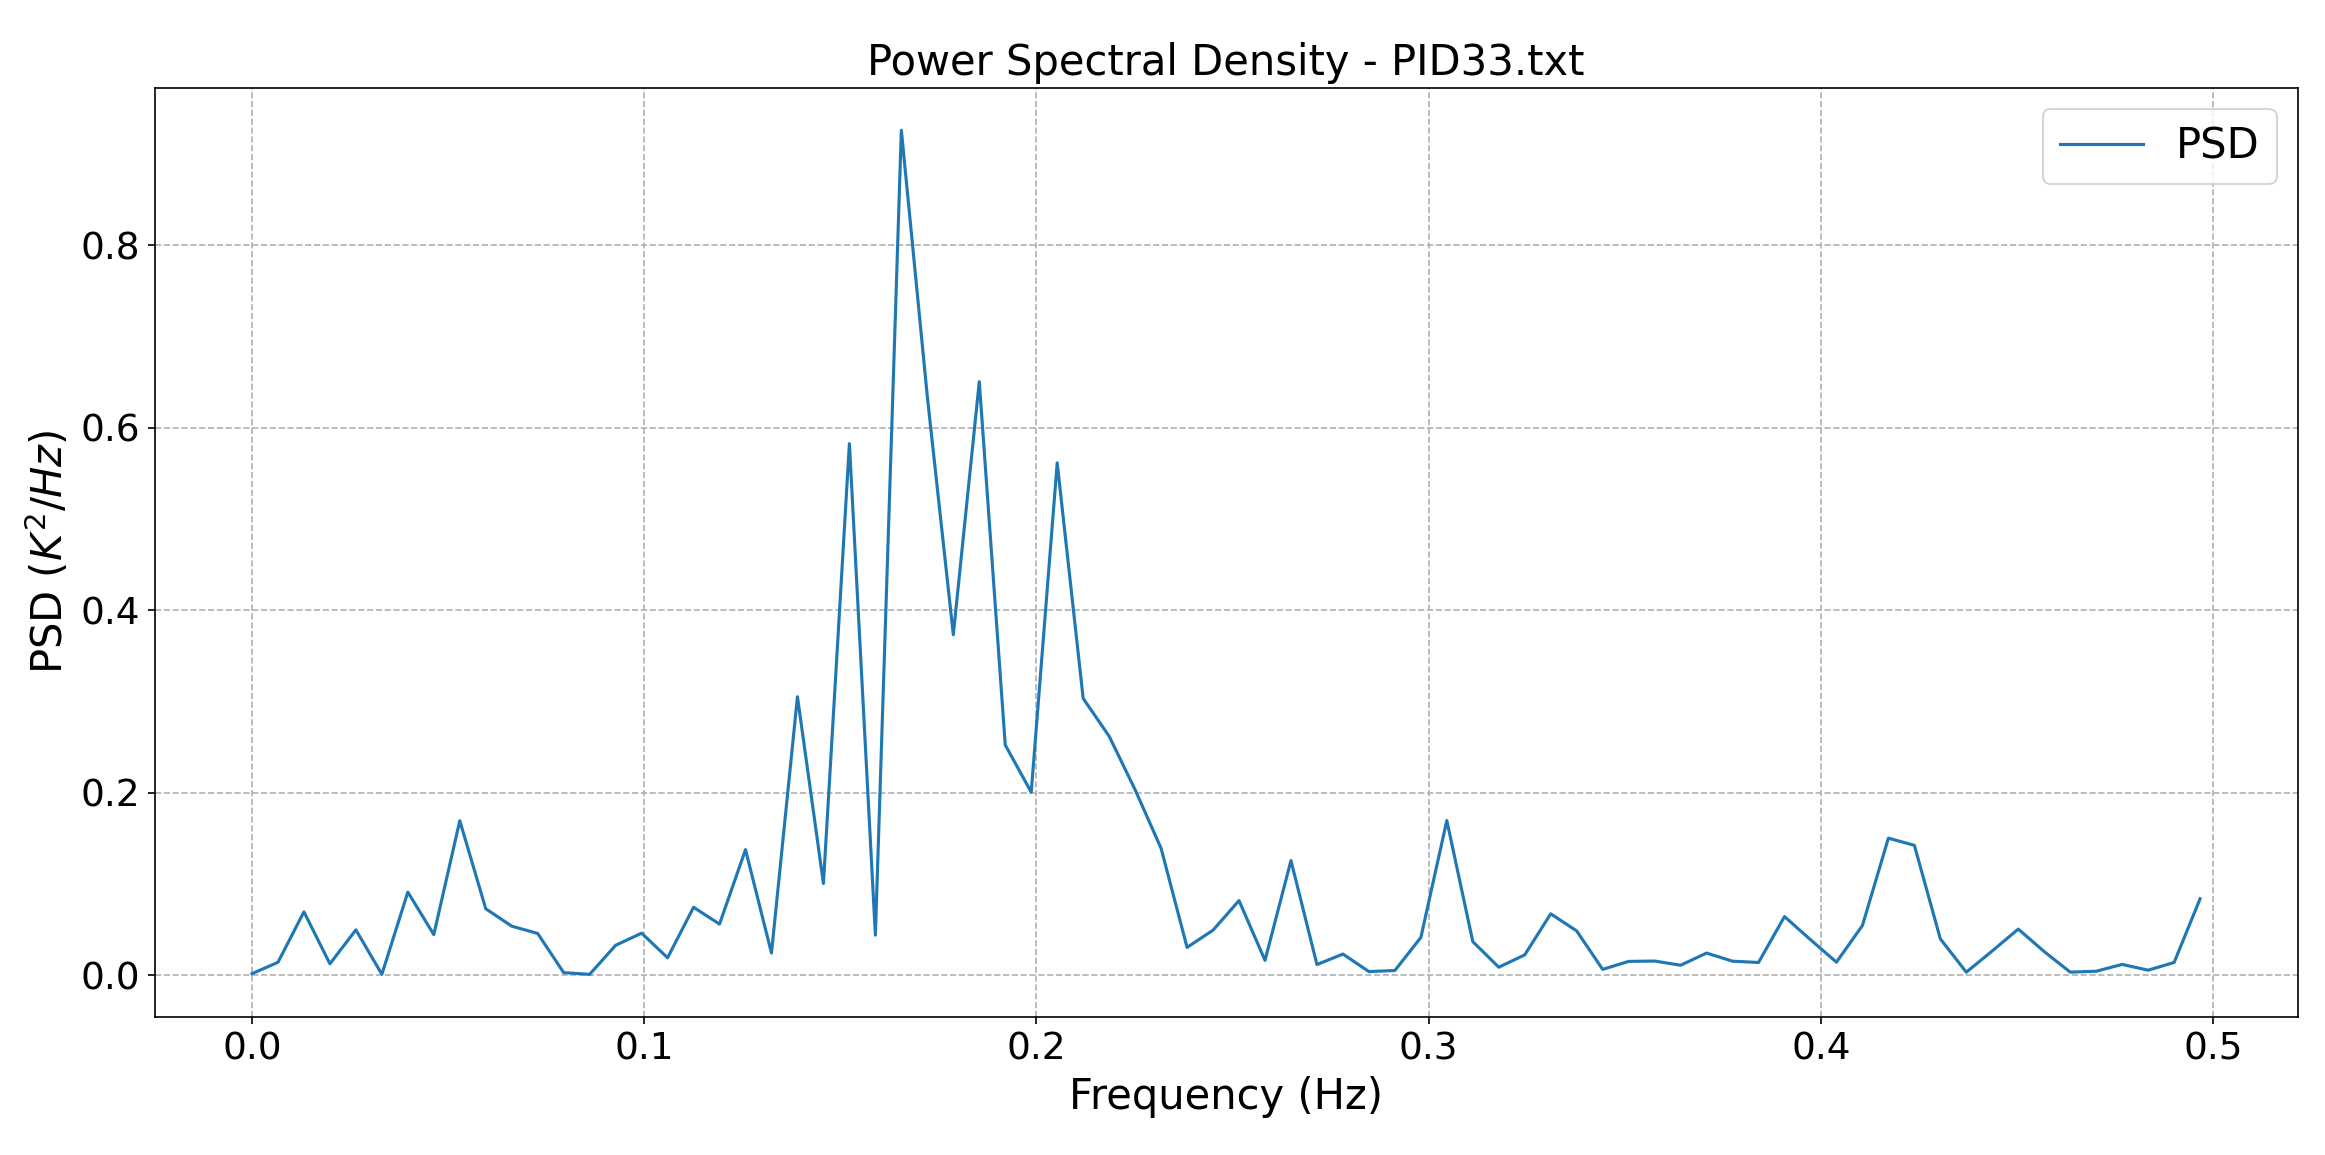
\includegraphics[width=0.6\linewidth]{PSDPID33.png}
		\caption{33℃PID控温PSD}
		\label{}
	\end{figure}
	%
	\subsubsection{数据频域图对数坐标}
	\begin{figure}[{H}]
		\centering
		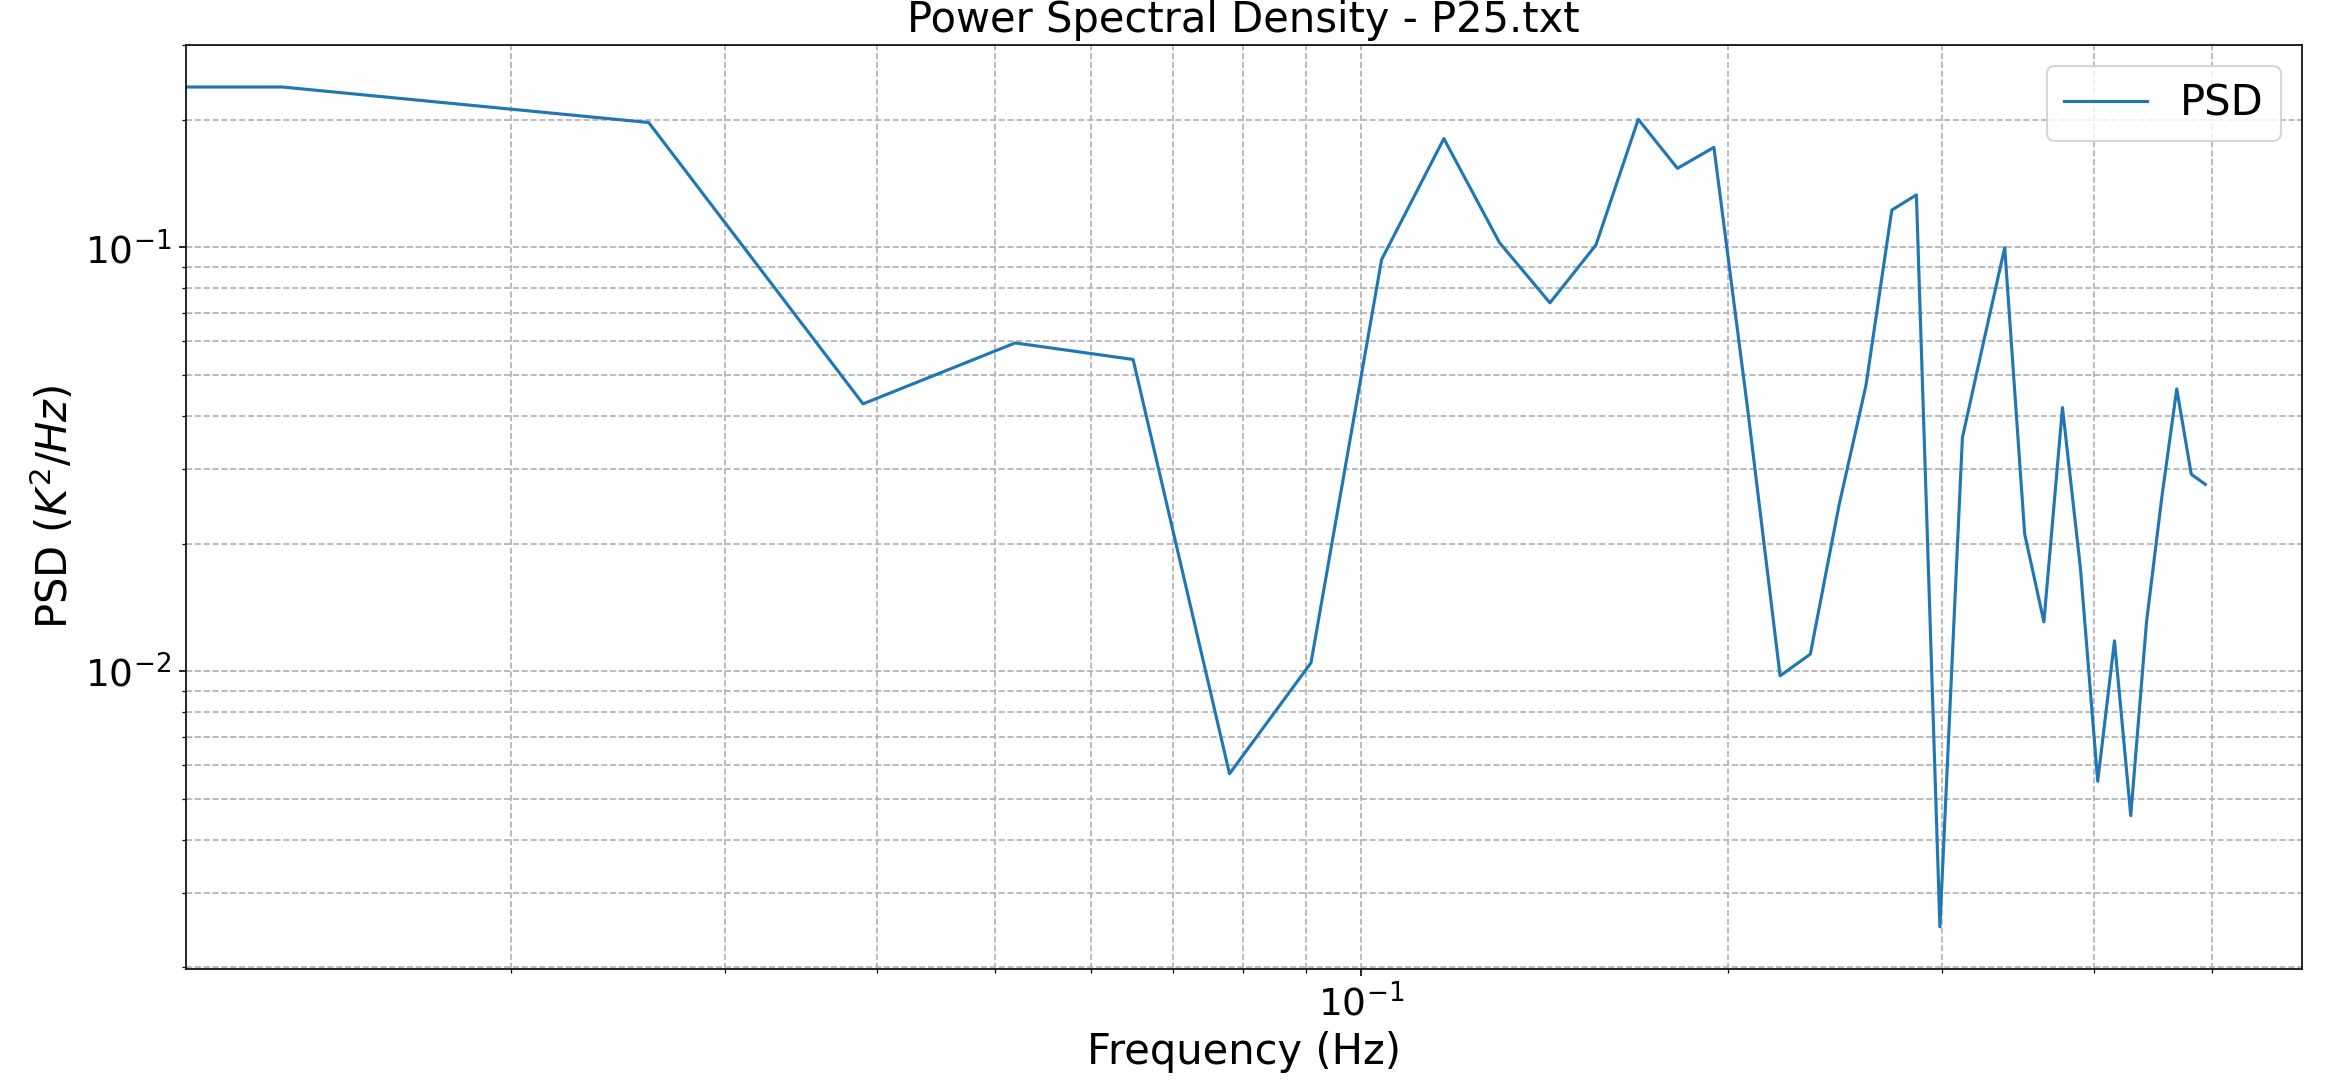
\includegraphics[width=0.6\linewidth]{LPSDP25.png}
		\caption{25℃P控温PSD}
		\label{}
	\end{figure}
	\begin{figure}[{H}]
		\centering
		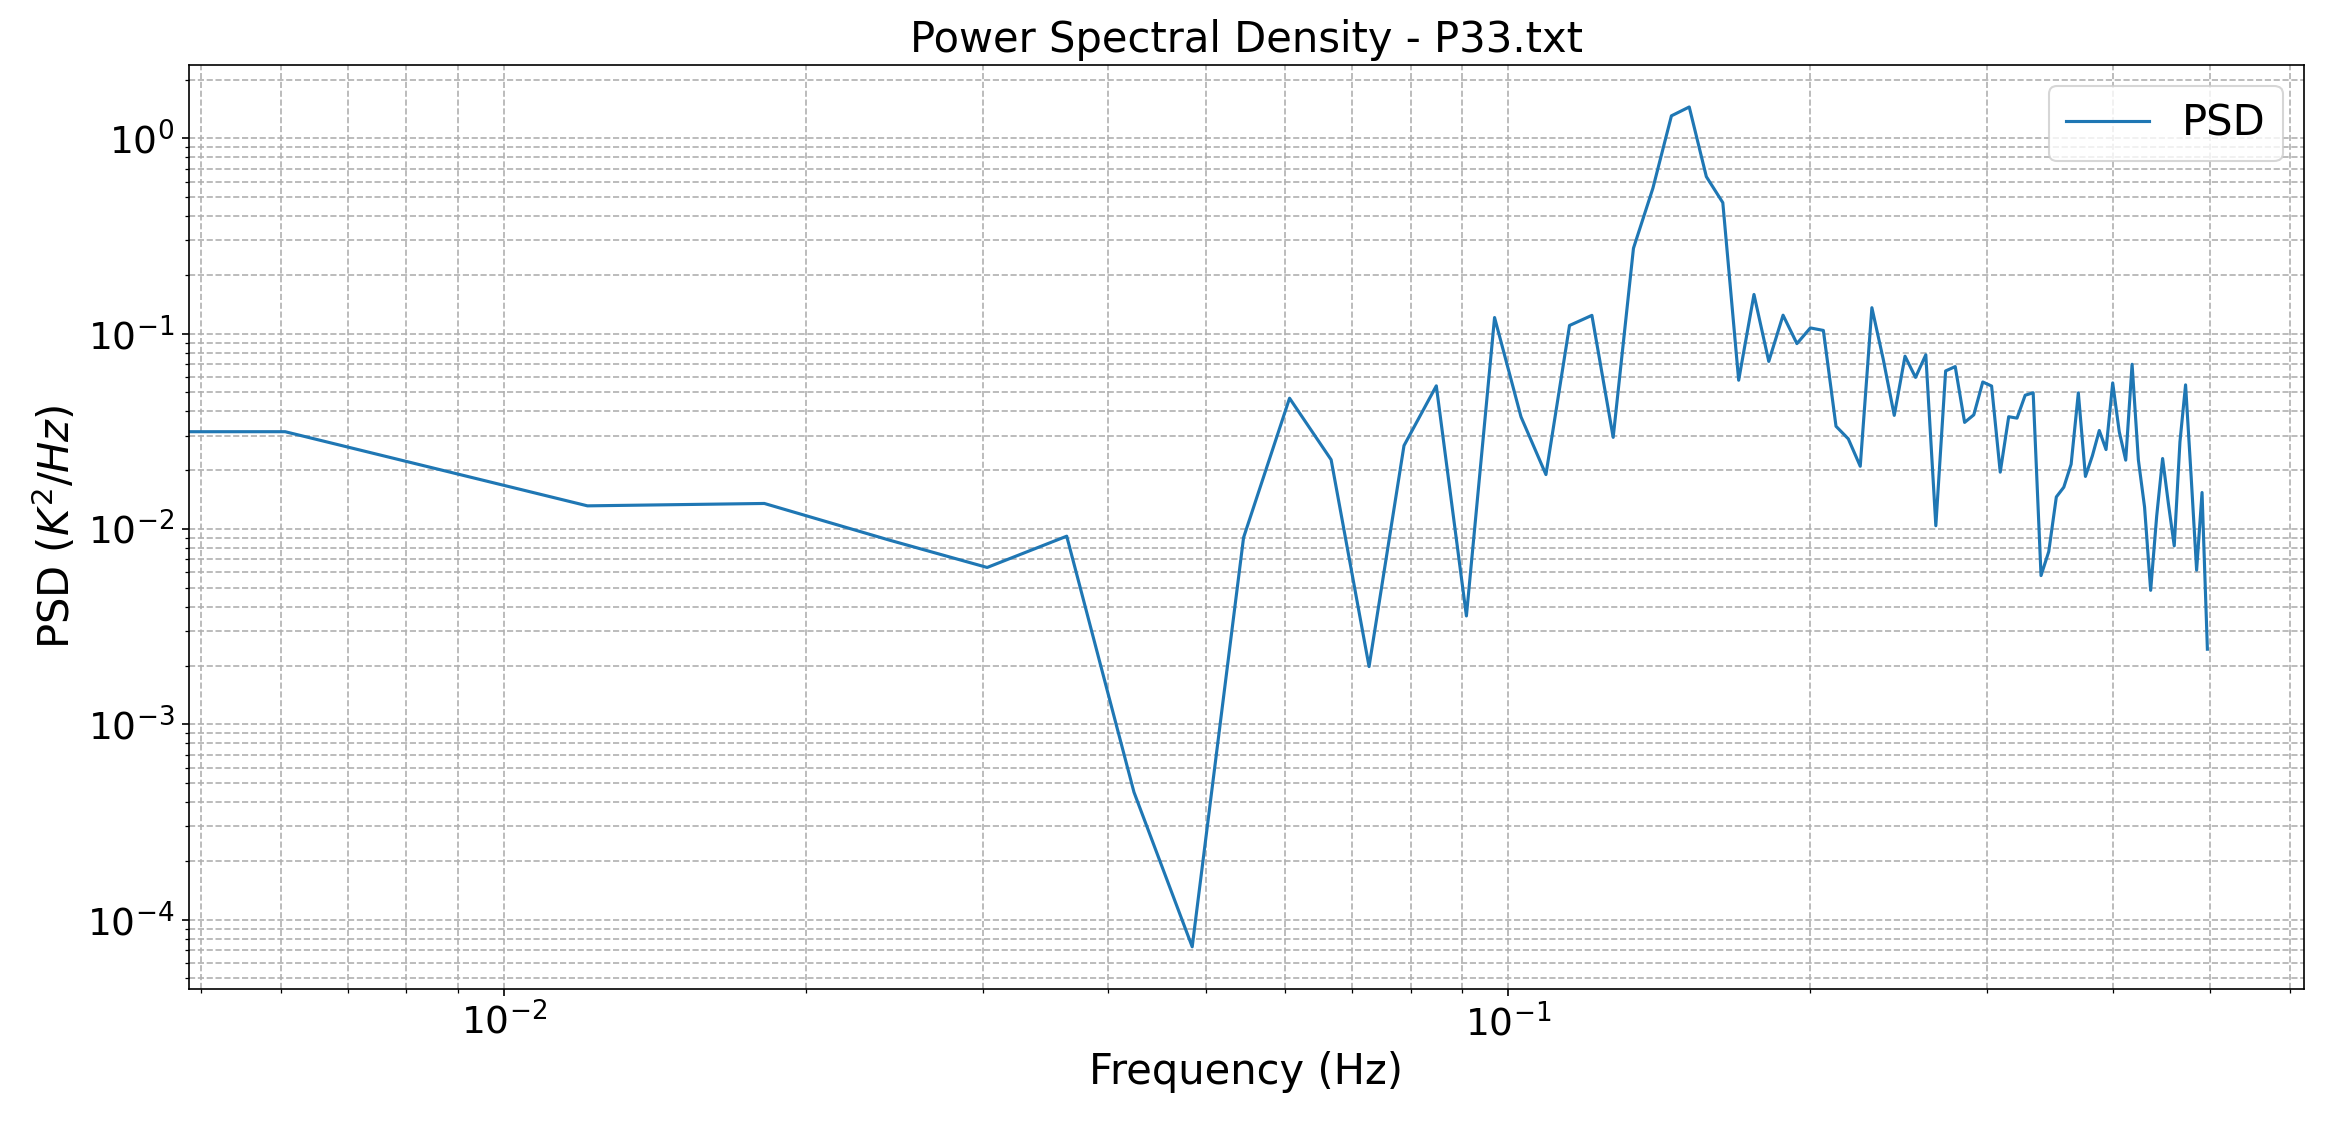
\includegraphics[width=0.6\linewidth]{LPSDP33.png}
		\caption{33℃P控温PSD}
		\label{}
	\end{figure}
	\begin{figure}[{H}]
		\centering
		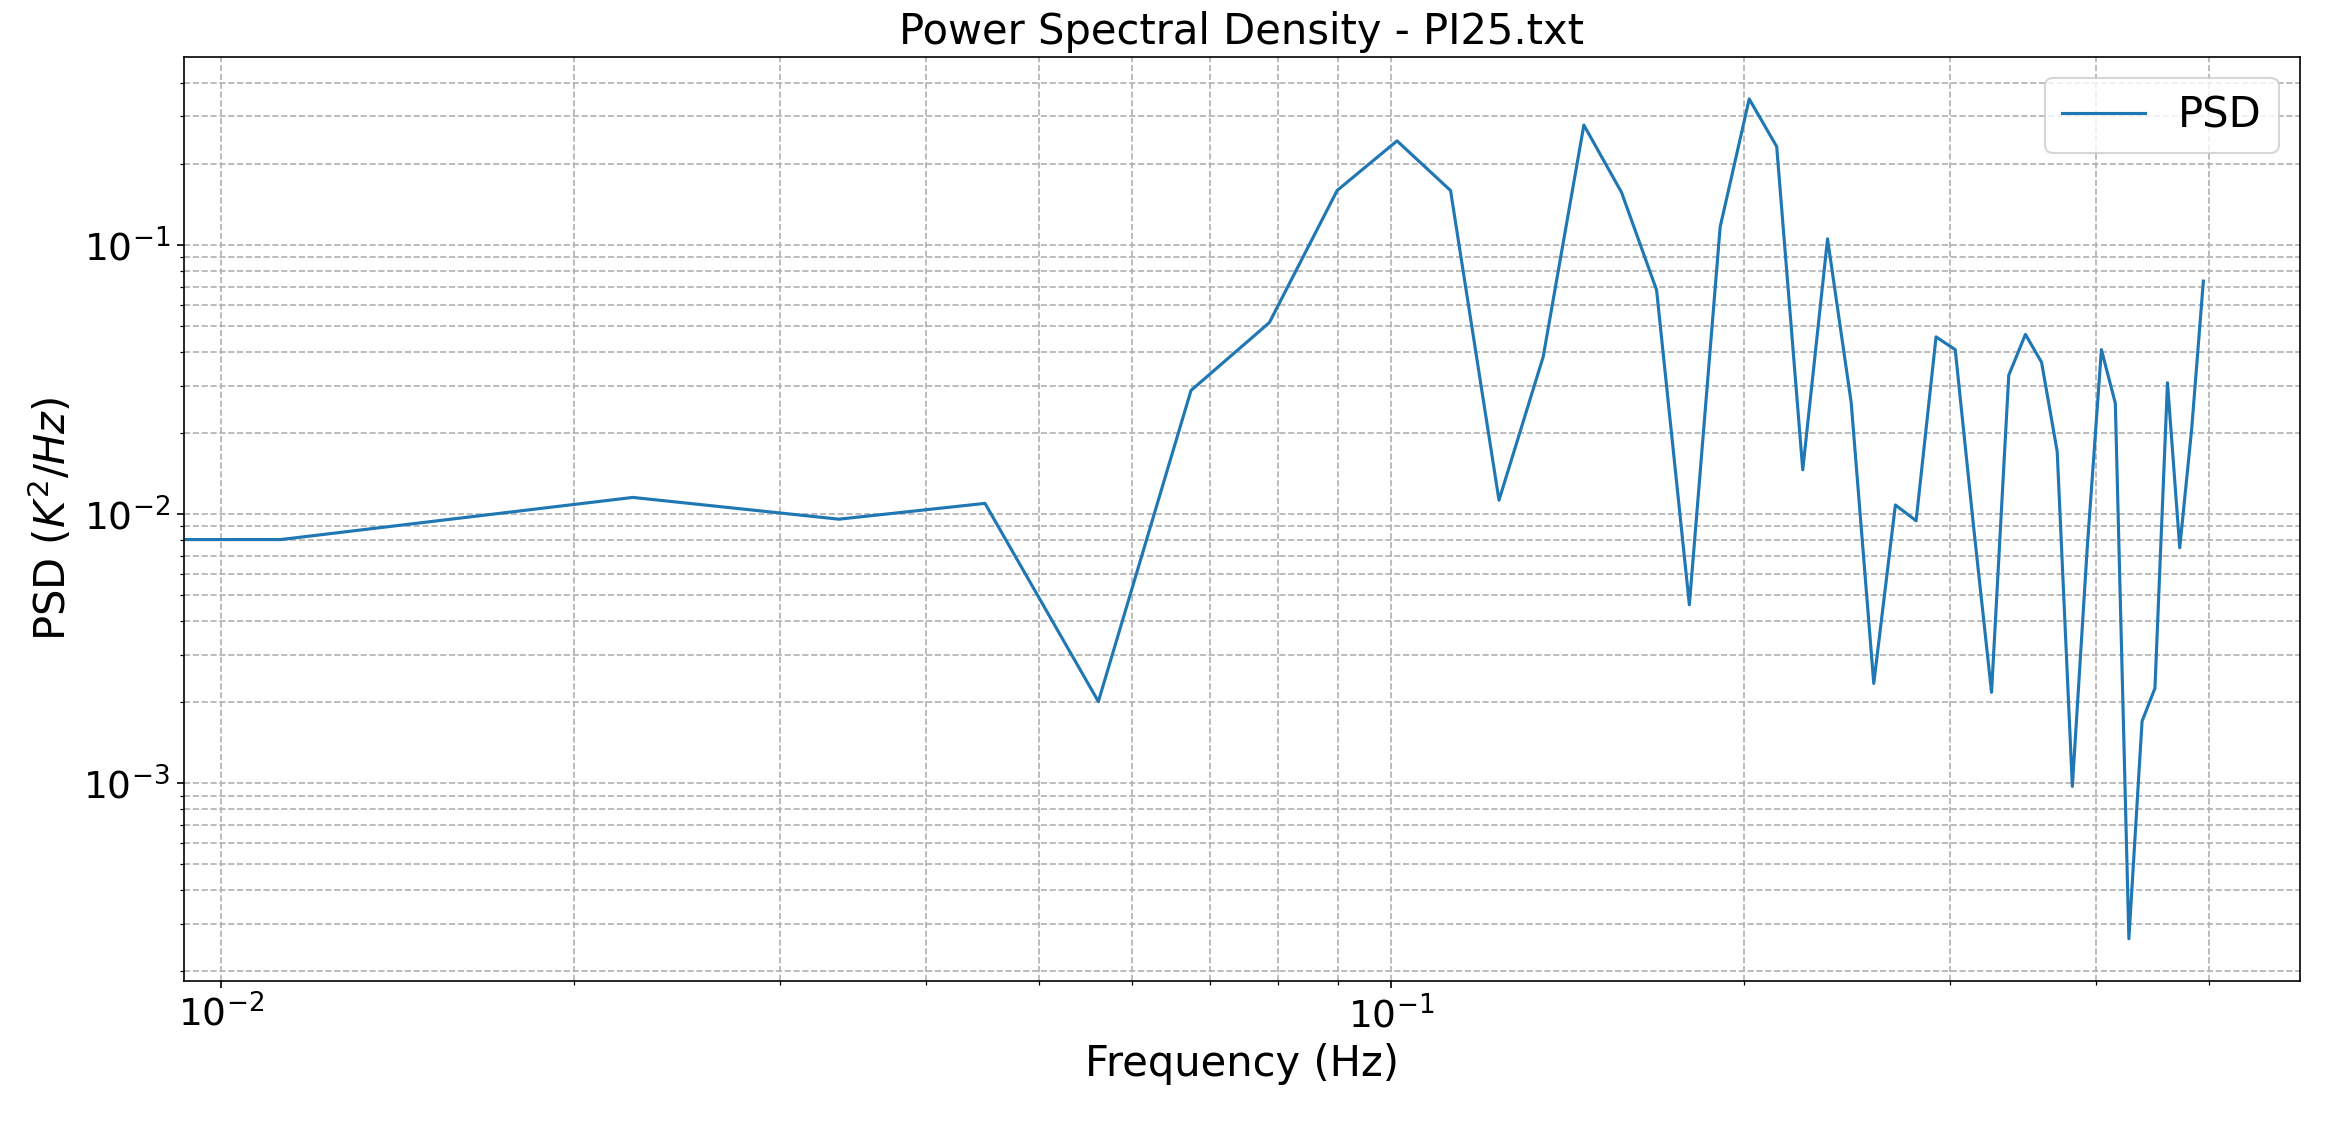
\includegraphics[width=0.6\linewidth]{LPSDPI25.png}
		\caption{25℃PI控温PSD}
		\label{}
	\end{figure}
	\begin{figure}[{H}]
		\centering
		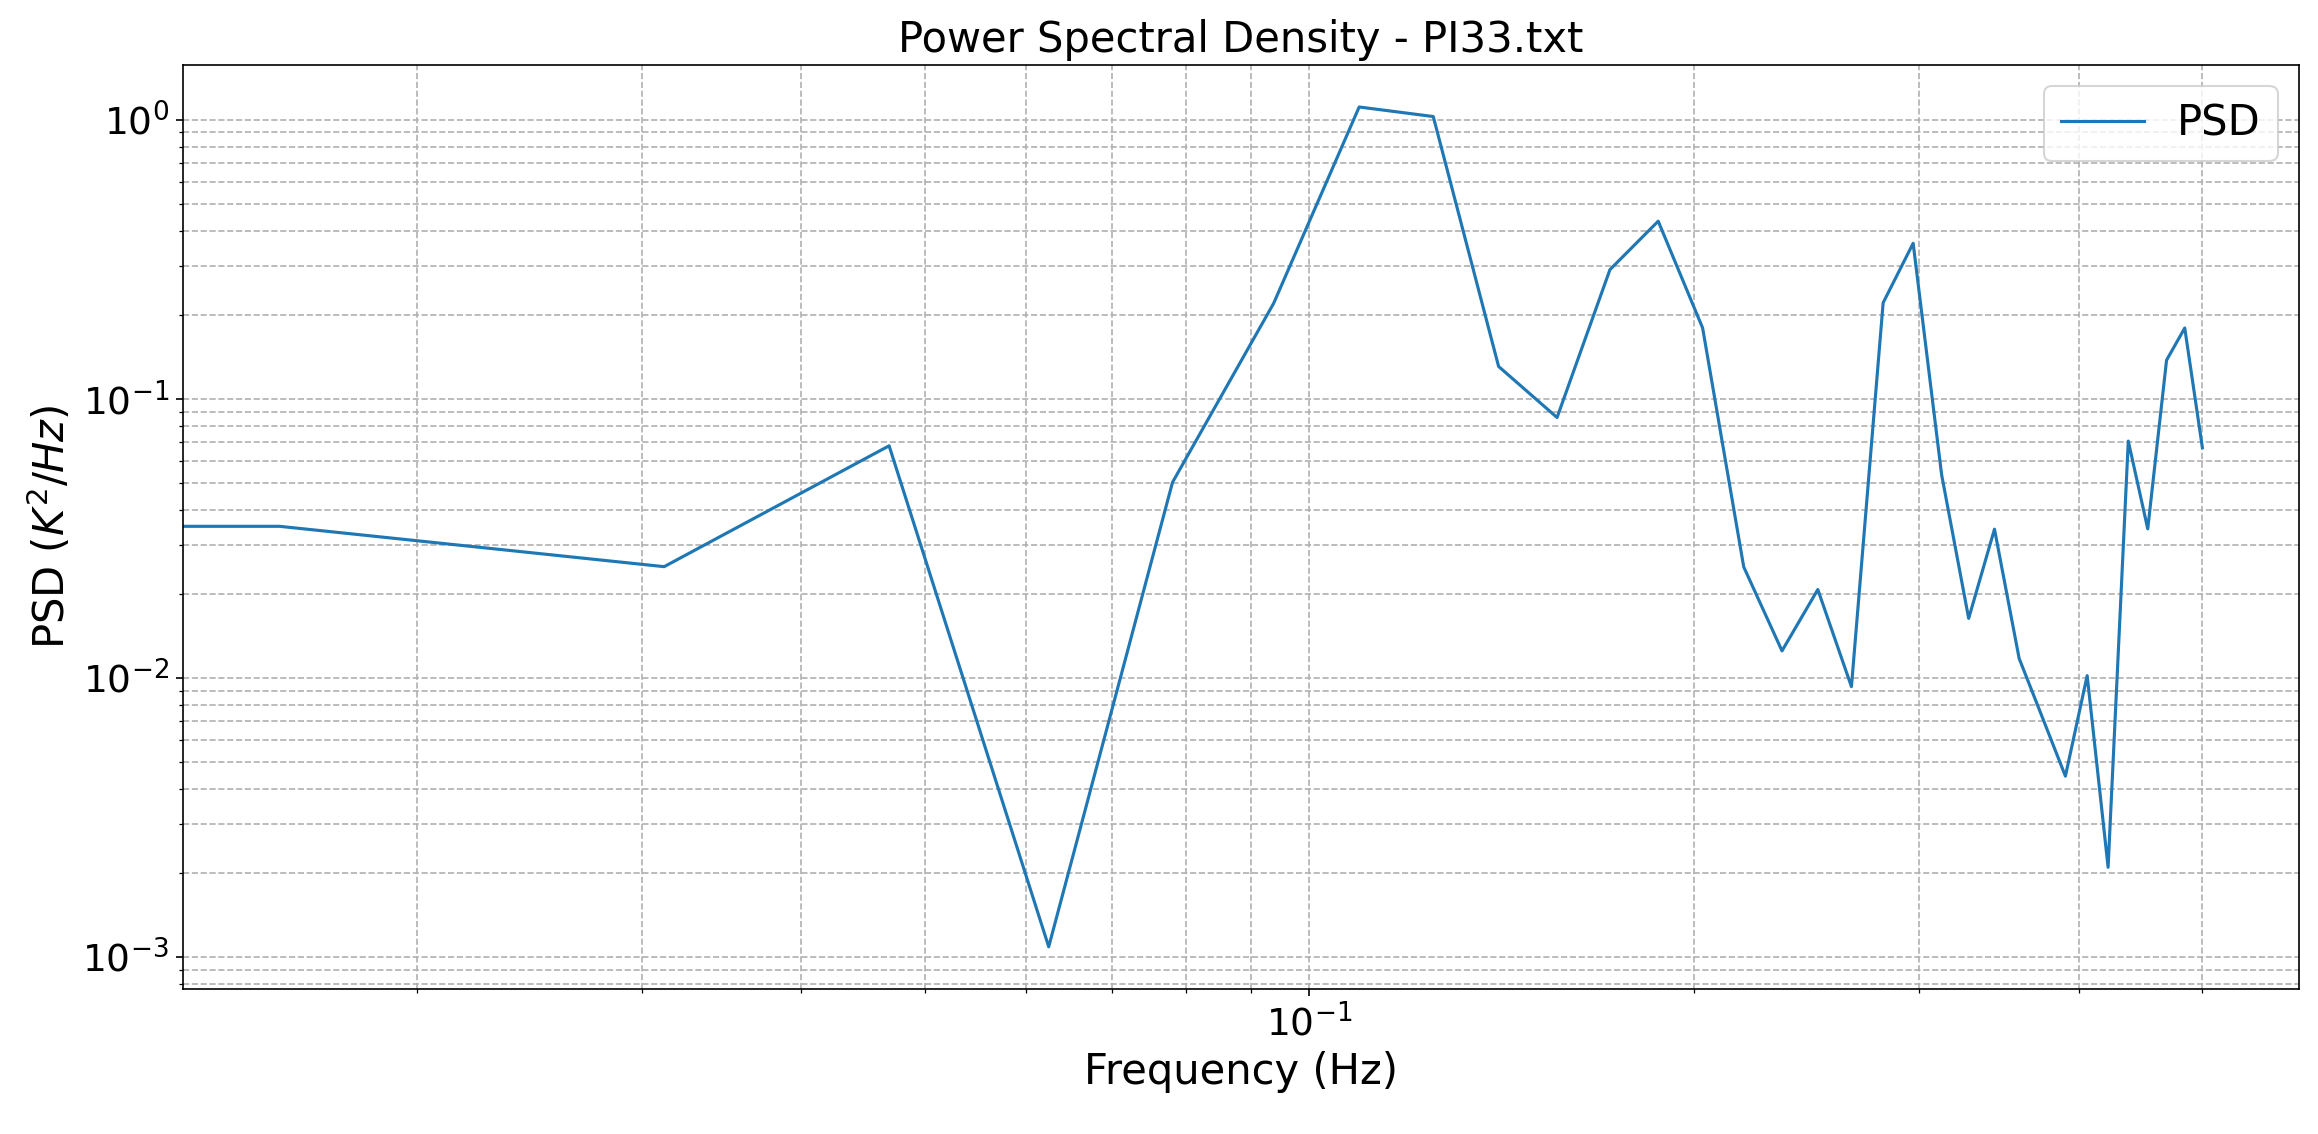
\includegraphics[width=0.6\linewidth]{LPSDPI33.png}
		\caption{33℃PI控温PSD}
		\label{}
	\end{figure}
	\begin{figure}[{H}]
		\centering
		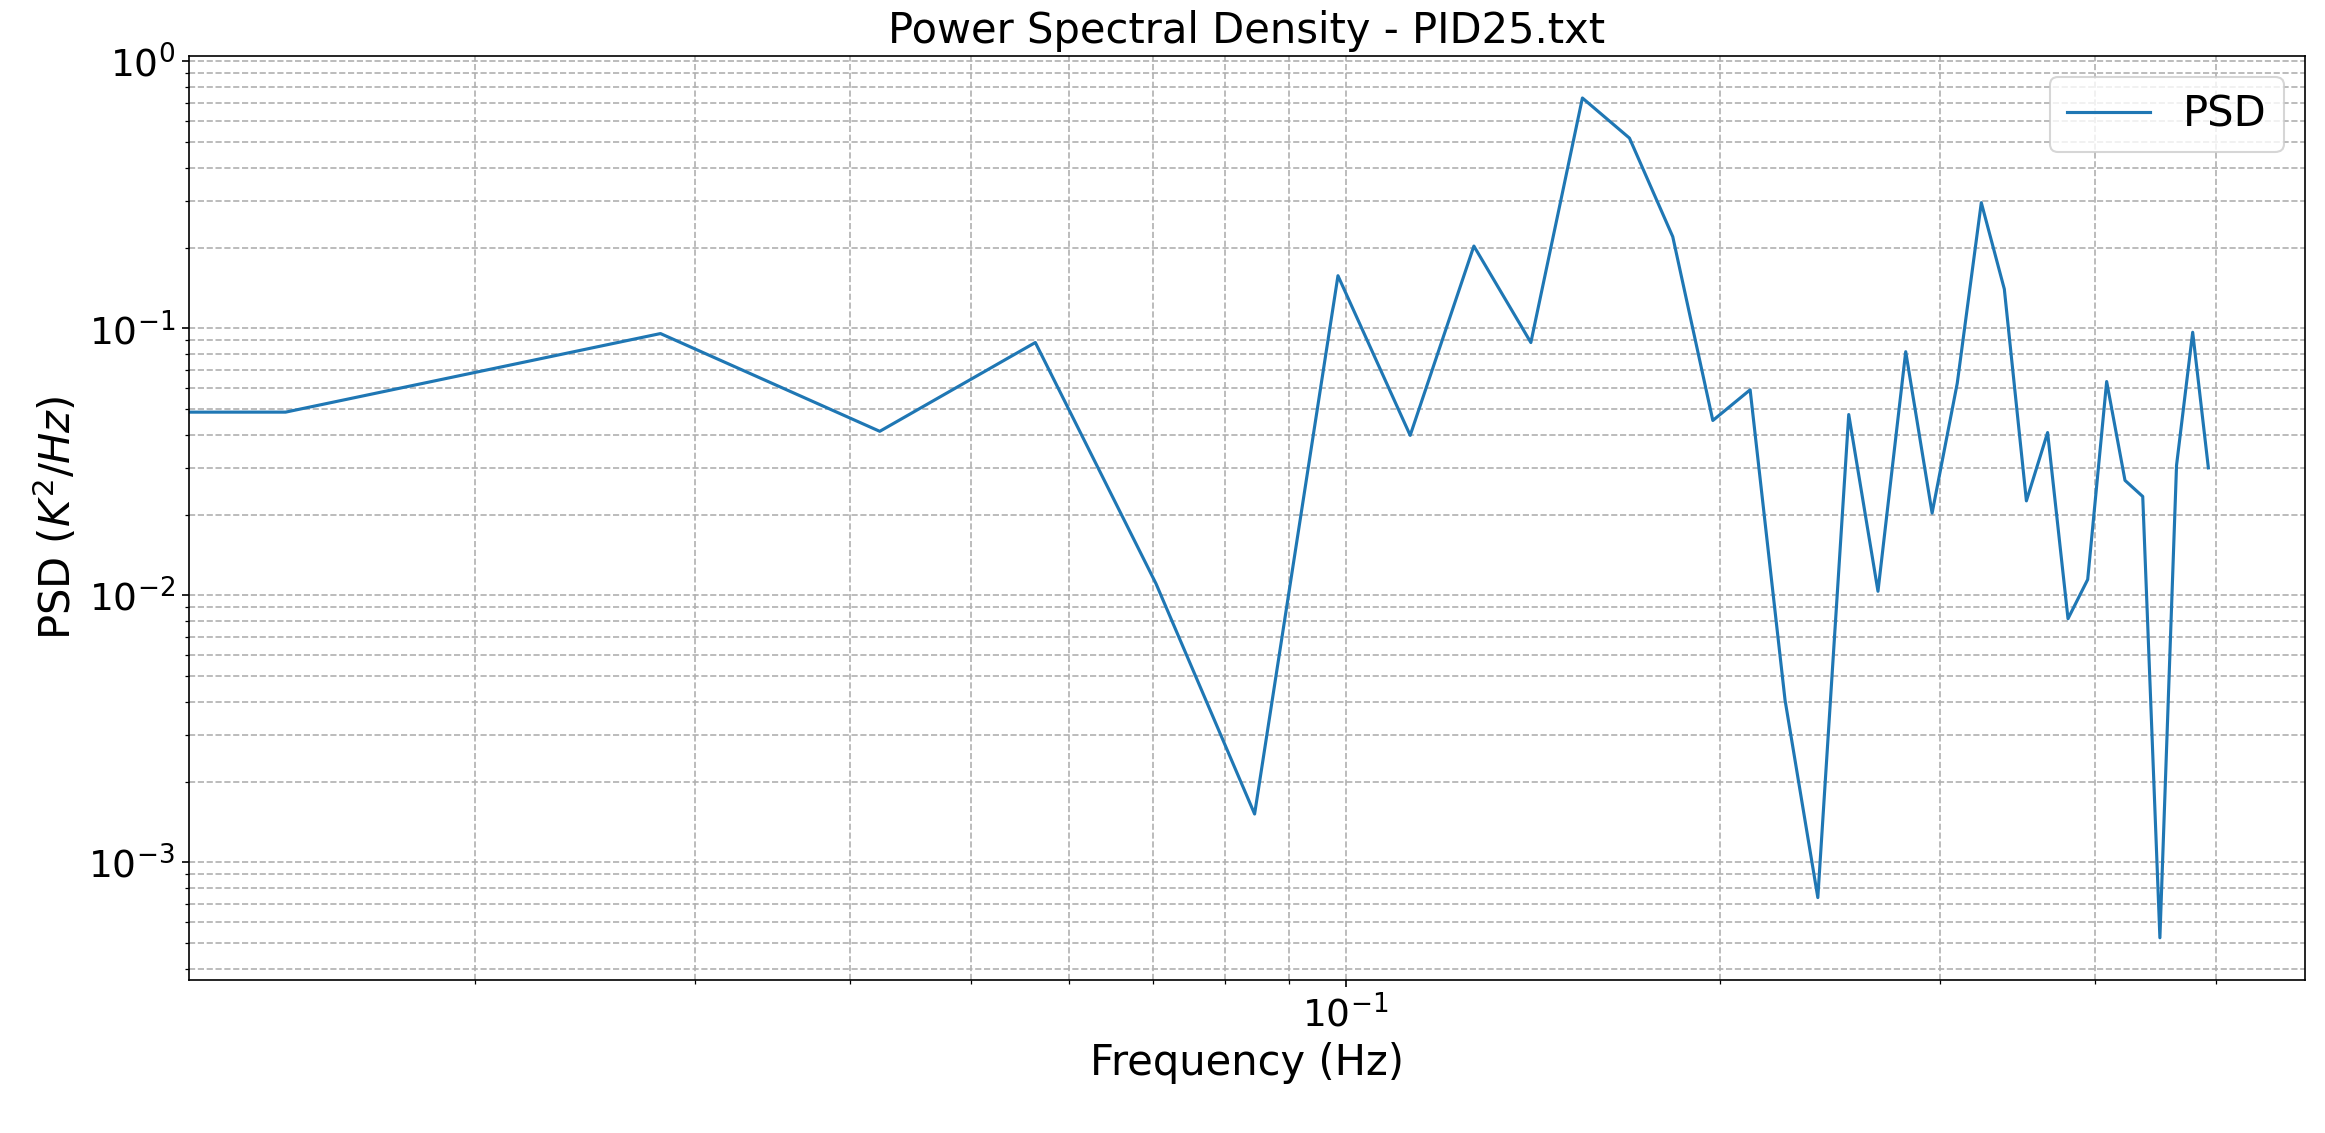
\includegraphics[width=0.6\linewidth]{LPSDPID25.png}
		\caption{25℃PID控温PSD}
		\label{}
	\end{figure}
	\begin{figure}[{H}]
		\centering
		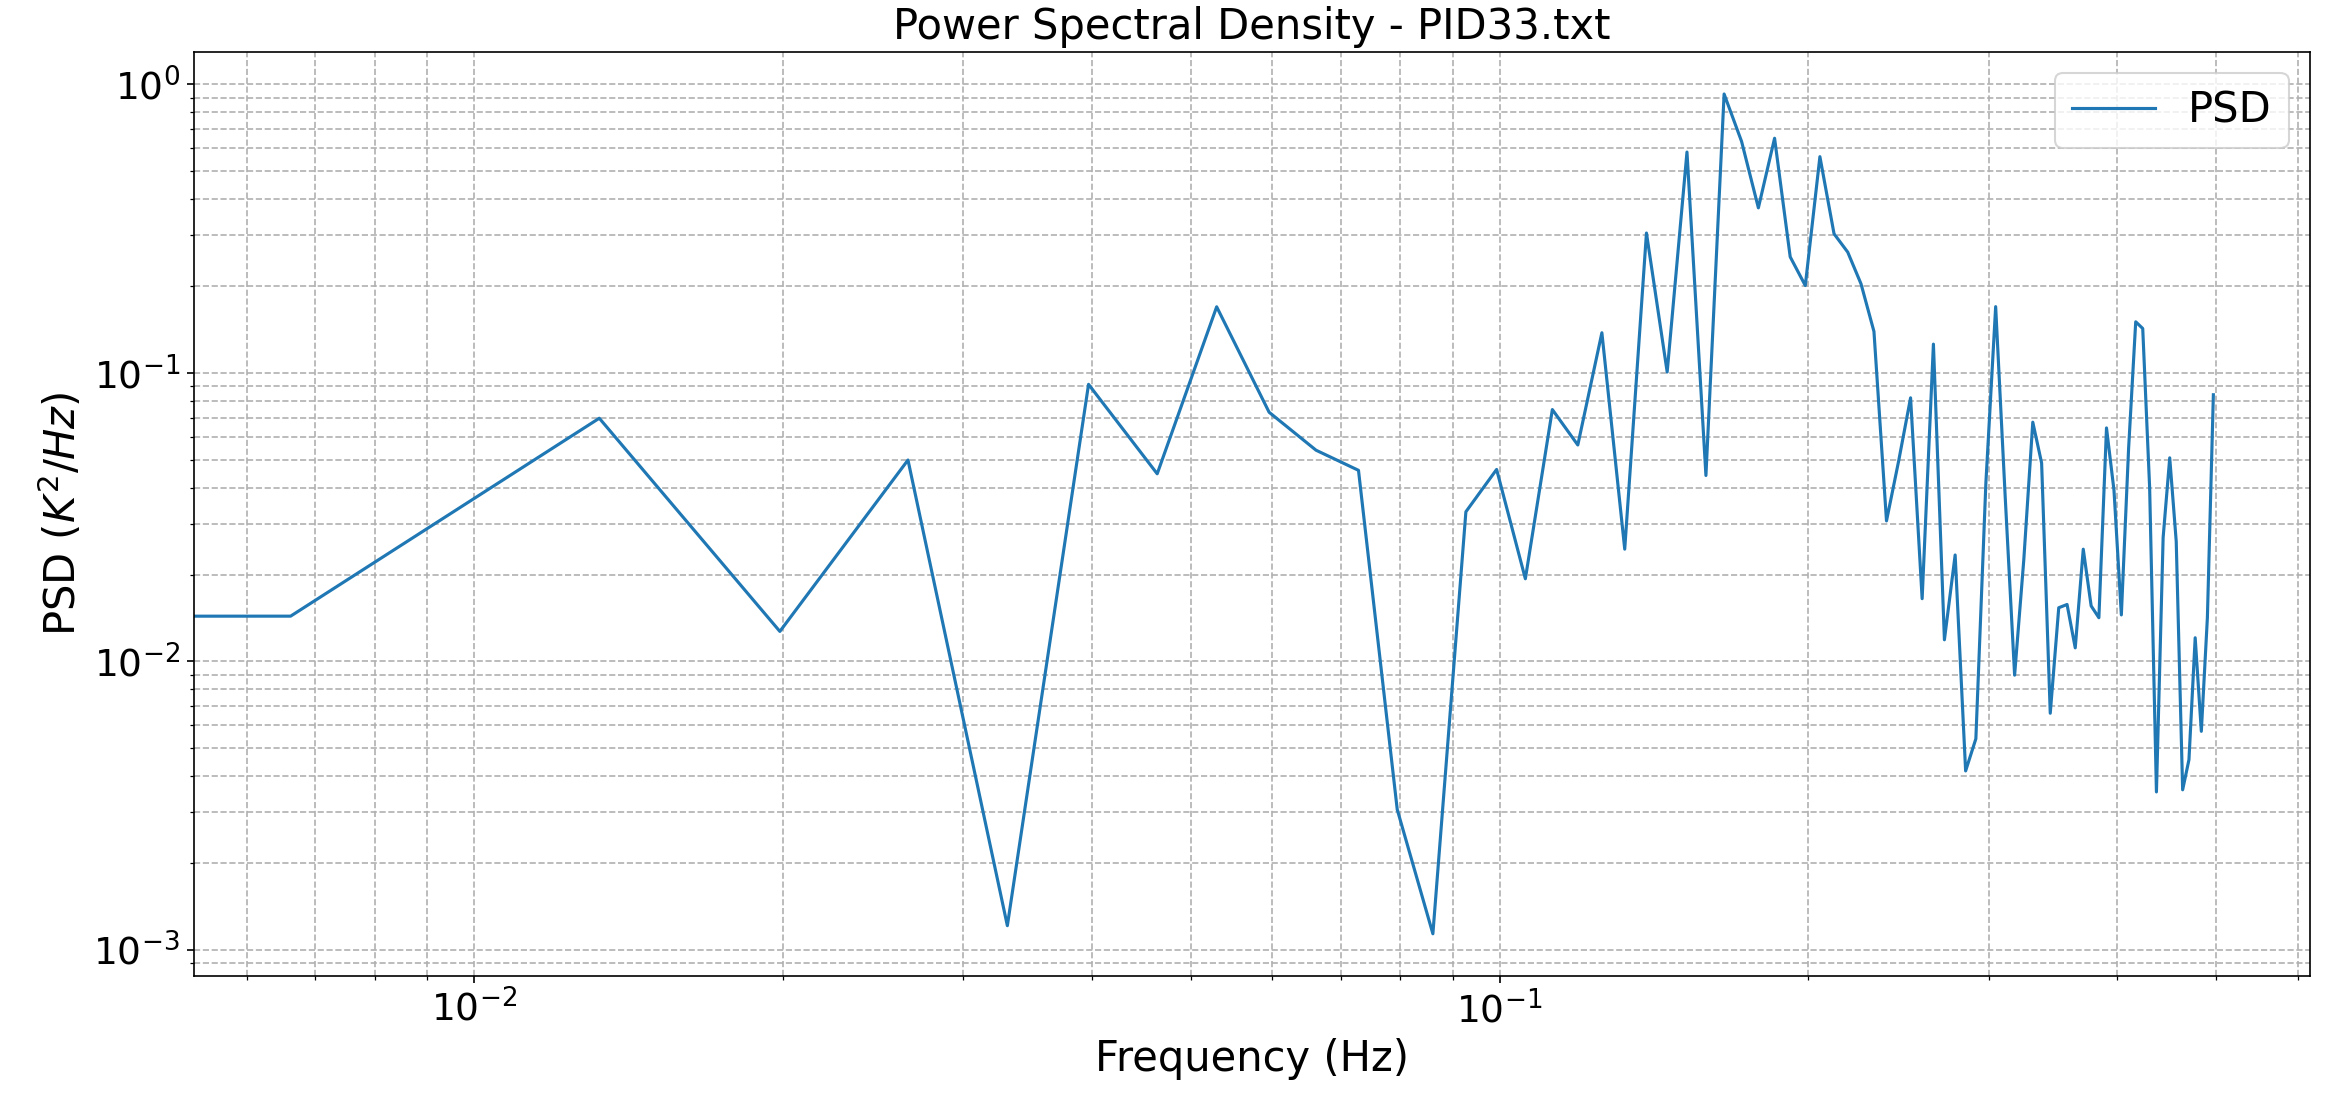
\includegraphics[width=0.6\linewidth]{LPSDPID33.png}
		\caption{33℃PID控温PSD}
		\label{}
	\end{figure}
	
	\subsection{时域数据分析}
	对实验相关数据进行误差分析,可以初步得出实验数据控温效果较好。
	\begin{figure}[{H}]
		\centering
		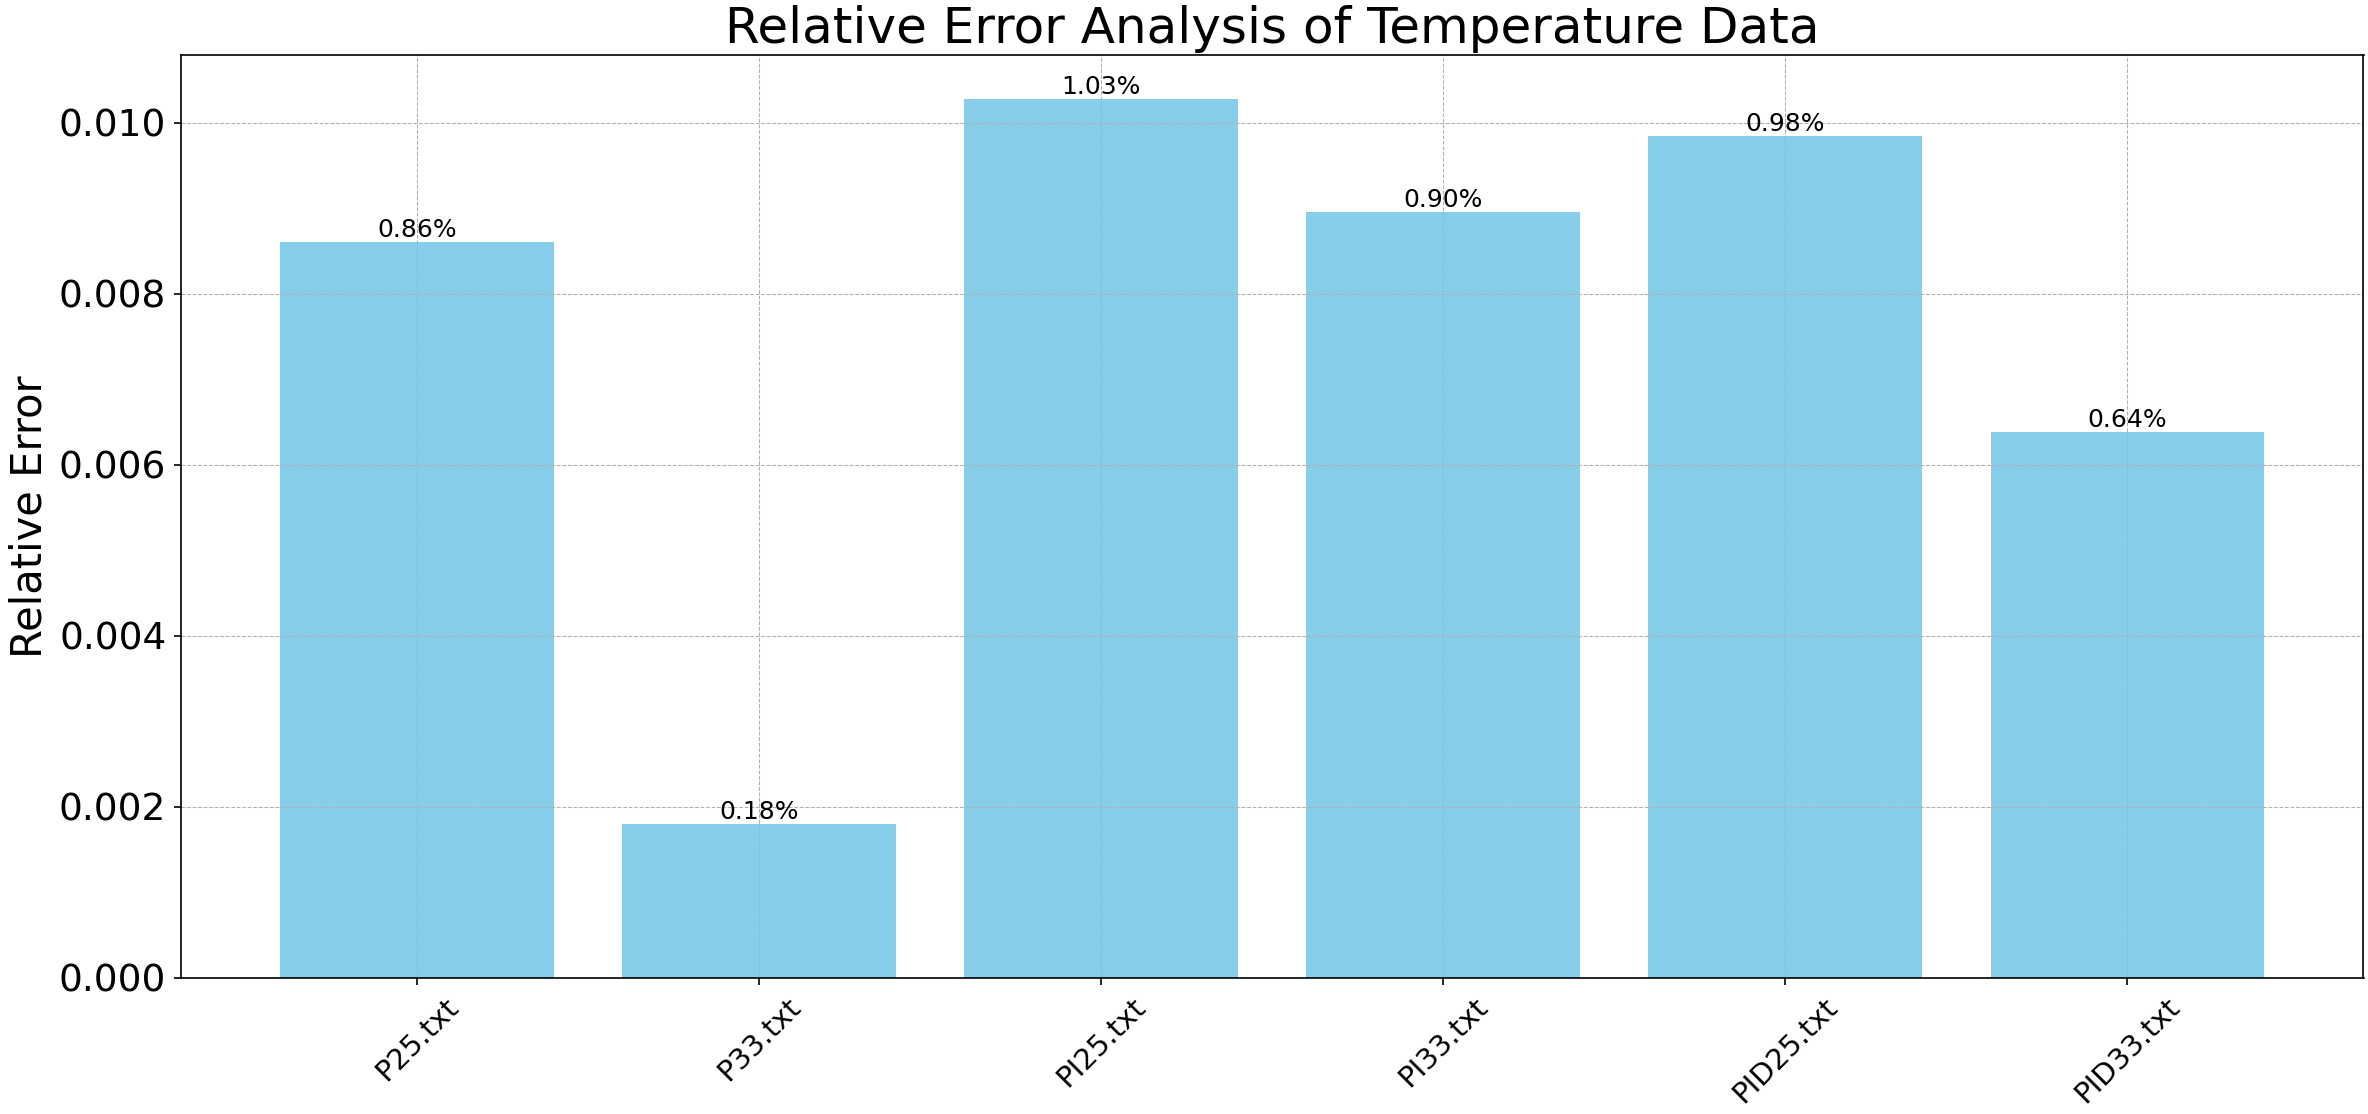
\includegraphics[width=0.6\linewidth]{相对误差.png}
		\caption{控温均值相对误差}
		\label{}
	\end{figure}
	于是随后进行的标准差的分析发现,PID控温并没有预期中控温效果更好,这可能是由于环境噪声的影响和参数调整。
	\begin{figure}[{H}]
		\centering
		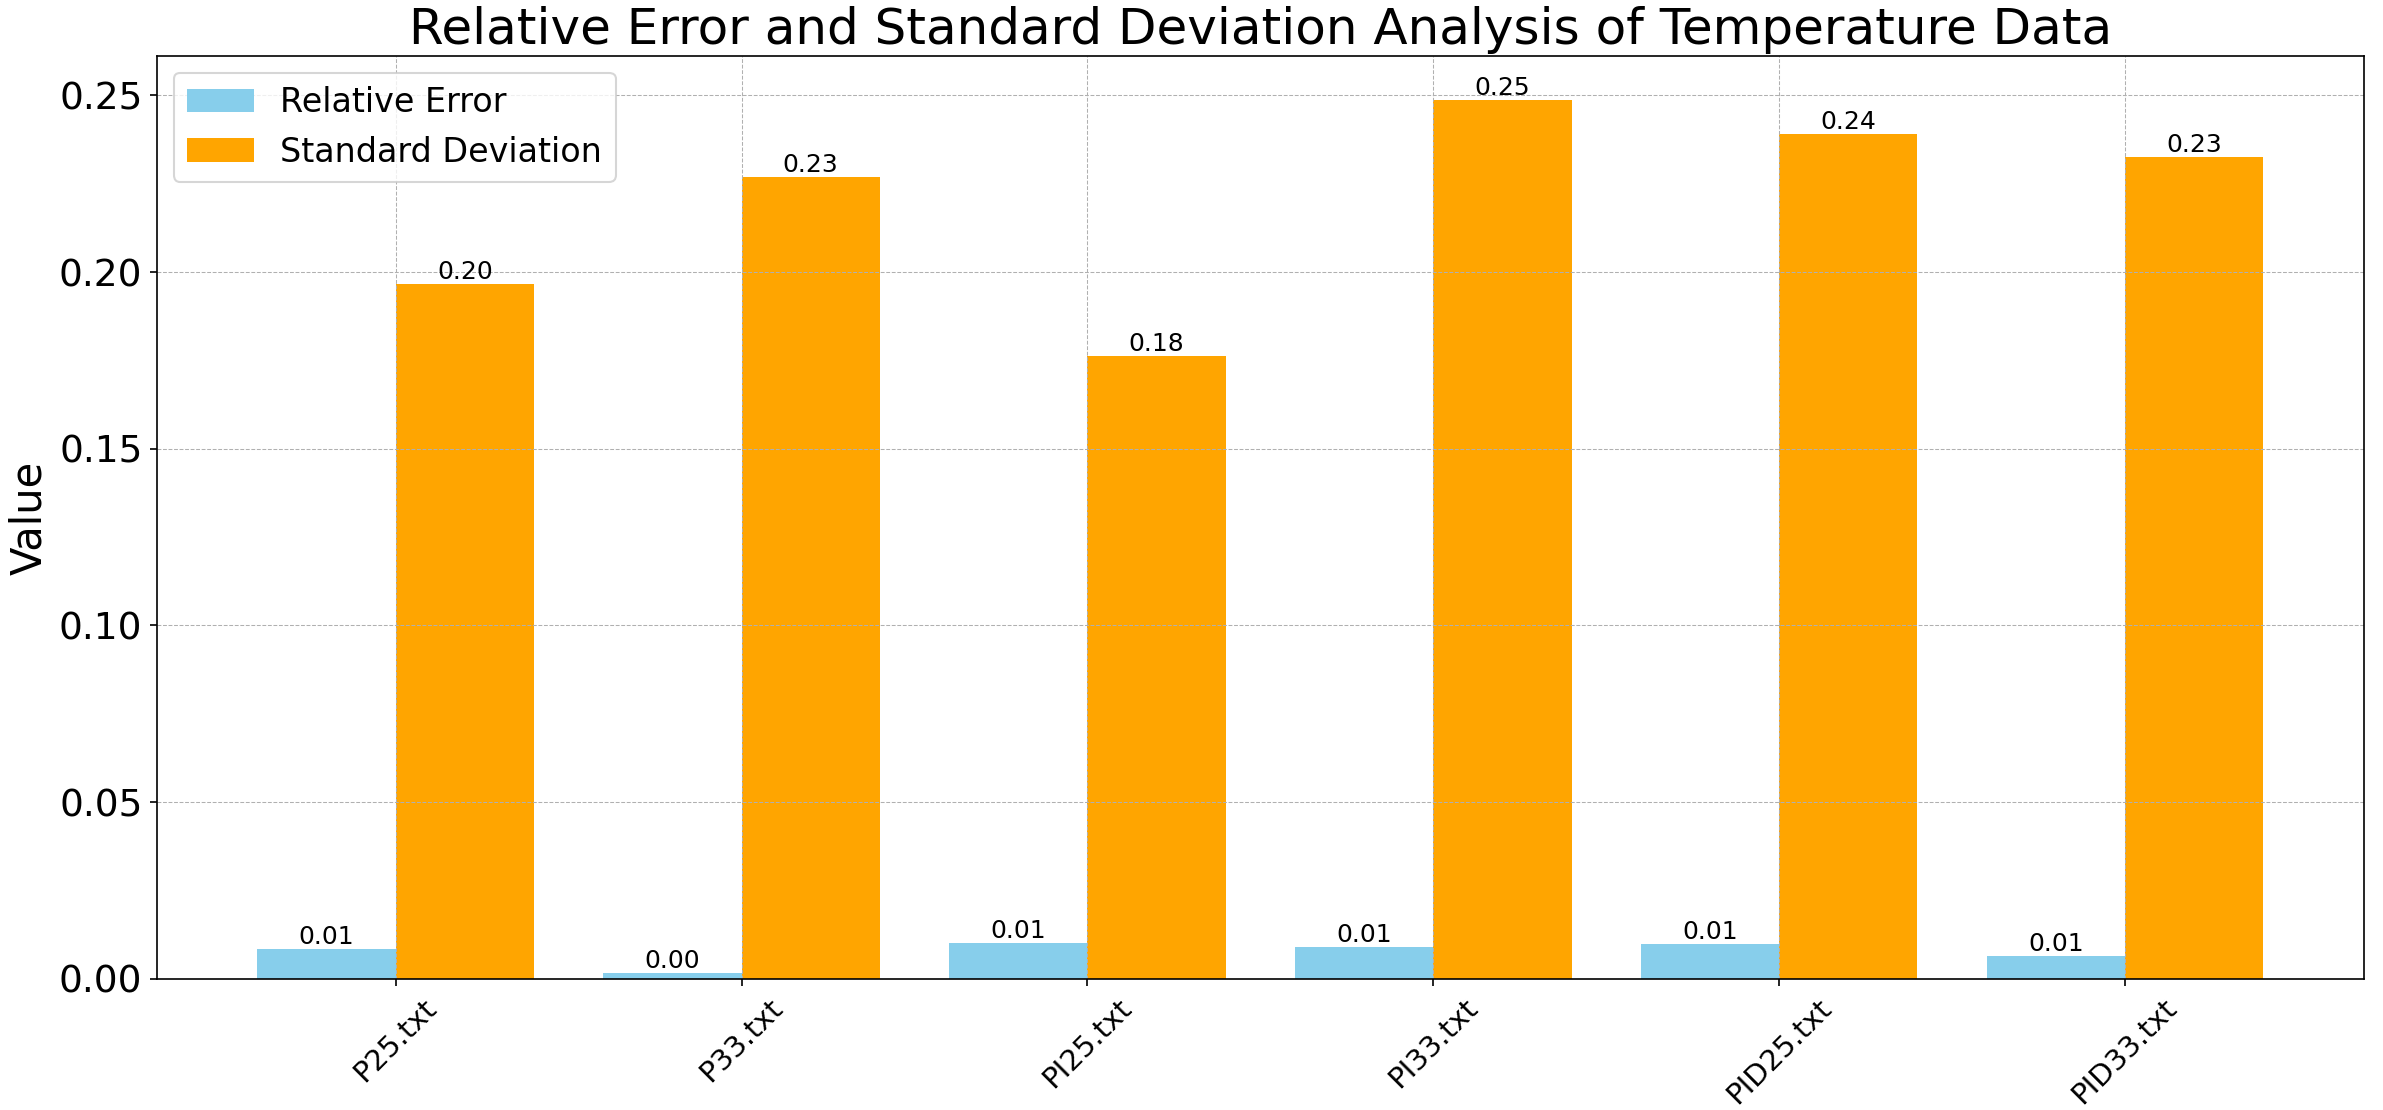
\includegraphics[width=0.6\linewidth]{误差2.png}
		\caption{相对误差与标准差}
		\label{}
	\end{figure}

	综合25℃和33℃两组实验数据来看,可以得出:

第一组25℃:

(1) P 控制:相对误差为 0.86\%,标准差为 0.20°C,温度波动最小,控温效果最佳。

(2) PI 控制:相对误差为 1.03\%,标准差为 0.18°C,温度波动稍大于 P 控制,但控温效果仍然较好。

(3) PID 控制:相对误差为 0.98\%,标准差为 0.24°C,温度波动较 PI 控制更大,控温效果略差于 PI 控制。

第二组33℃:

(1) P 控制:相对误差为 0.18\%,标准差为 0.23°C,温度波动最小,控温效果最佳。

(2) PI 控制:相对误差为 0.89\%,标准差为 0.25°C,温度波动略大于 P 控制,但控温效果仍然较好。

(3) PID 控制:相对误差为 0.64\%,标准差为 0.23°C,温度波动略大于 P 和 PI 控制,控温效果稍差。
\subsection{频域数据分析}


第一组(设定控温温度25°C):
 
图19中,能量分布较高,系统存在较大的波动,系统慢速响应。
 
 图21中,低频段能量分布较低,显示系统对低频扰动的良好抑制效果,控温效果较好。

 图23中,全频段的能量分布均较低,控温效果极佳。

第二组(设定控温温度33°C):

	图20中,低频段的能量分布较高,显示系统存在较大的温度波动,响应较慢。

图22中,低频段和中频段的能量分布较低,整体波动较小,控温效果较好。

图24中,低频段和中频段的能量分布均较低,控温效果最佳。

综上所述,添加积分和微分控制参数(PI和PID控制)能够有效降低温度波动,提升稳定性。
\subsection{控温效果总结}
\textbf{对于时域数据的分析体现出PID控温并没有想象中那么优秀,反而其标准差较大与其余两种控温方式没有多少区别。而在频域图上进行分析时就可以明显看出PID与其余两种方式的优越之处,而之所以能得出符合客观实际的PID控温优秀的结论,是基于时域数据相差不大,频域数据更加优秀的基础上的。}


实验中有很多噪声的引入导致了实验数据的不稳定,这一点对于实验数据来说是影响很大的,所以需要更多的在稳定的环境中进行实验,方可能得出与理论相符的实验结果。
	% 实验后思考题
	\subsection{实验后思考题}
	
	%思考题1
	\begin{question}
		影响控温精度和稳定度的因素都有哪些, 如何进行改进?
	\end{question}
	影响控温精度和稳定性的因素包括以下几个方面:首先,TEC(热电制冷器)的性能至关重要,选择合适功率、制冷能力和温度范围的TEC能直接提升控温系统的稳定性和精度。其次,环境温度和散热效率也会影响TEC的工作状态,进而影响控温效果,因此良好的散热设计和环境温度控制是必要的。此外,传感器的准确性和灵敏度对控温系统的精度有直接影响,选用高精度、高灵敏度的传感器并进行校准能够提高系统性能。最后,控制算法的设计对控温系统的影响很大,采用合适的PID控制算法并根据实际情况进行参数调整,可以提升控温的稳定性和精度。

	为改进控温系统的性能,可以采取以下措施:优化散热设计,提高散热效率,从而减少环境温度对TEC系统的影响;选择高精度、响应速度快的传感器,并进行精确校准,确保其准确性和稳定性;针对不同的实验需求,改进控制算法设计,采用合适的PID参数调整策略,以提高控温系统的整体性能。
	% 思考题2
	\begin{question}
		本实验中直流电源的电流输出建议设置为 2A, 为了减小温度的波动, 电流设置应该增大还是减小, 为什么?
	\end{question}
	增大直流电源的电流输出有助于减小温度的波动。这是因为TEC(热电制冷器)的制冷或制热能力与电流成正比关系。增大电流可以提高TEC的制冷或制热功率,从而使其能够更快速地响应温度变化,进而实现更精确的温度控制。

当温度波动较大时,增大电流输出可以增加TEC的制冷量或制热量,使系统更能够快速地回到设定温度。这样可以有效地抑制温度的波动,提高控温系统的稳定性。

然而,需要注意的是,过大的电流可能会引起系统的过冲和振荡,从而增加温度波动。因此,在增大电流输出时,需要在系统稳定性和响应速度之间找到平衡。通过适当调节电流大小,可以在提高系统响应速度的同时,避免引入过大的振荡,从而实现更稳定的温度控制。
	% 思考题3
	\begin{question}
		实验是否达到了控温的目的, 还有哪些可以改进的地方?
	\end{question}
	根据实验数据分析可知,实验达到了控温的目的。

	在实验中实现更好的控温效果,可以考虑以下改进方面:

参数优化:对控制系统中的参数进行优化调整,如PID控制器中的比例、积分、微分参数,以提高系统的响应速度和稳定性。

传感器校准:确保使用的温度传感器准确性高且稳定,可以进行定期的校准和调试,以减小温度测量误差。

散热设计:进一步优化散热系统,提高散热效率,以降低环境温度对控温系统的影响,从而减小温度波动。

	\begin{question}
		温度控制程序是否工作正常, 是否还有优化的地方?
	\end{question}
	有两种不同的温度控制程序,其中一种无法进行工作,从界面显示发现明显缺少关键记录仪器,而第二种软件使用较为流畅,但是存在记录数据计算较慢,可以进行优化算法。

	此外实验中的环境噪声很大,可以在程序中加入滤波器来屏蔽掉一部分噪声。
	% ---
	
	
	% 结语部分
	\clearpage
	
	% 小标题
	\section{TEC控温实验\quad\heiti 结语}
	% ---
	
	% 总结、杂谈与致谢
	\subsection{实验心得和体会}
	\begin{enumerate}
		\item 实验接线较为困难,并且进行运行程序的时候也出现了问题,不得不更改使用的程序,之后的问题是,实验温度的测量会受到环境的影响,并且影响非常大,比如说桌子的震动甚至都会影响输出的数据。
		\item 实验中由于许多困难的存在,导致实验的时间很长很长才能获得足够进行分析的实验数据。
		\item \textbf{本实验报告采用LATEX编辑,实验分工为黄罗琳同学负责实验操作、记录数据、编辑报告、数据绘图,数据分析,丁侯凯同学负责实验操作、数据绘图、数据分析。}
	\end{enumerate}
	
	

	% 附件
	\subsection{附件}
\begin{figure}[{H}]
	\centering
	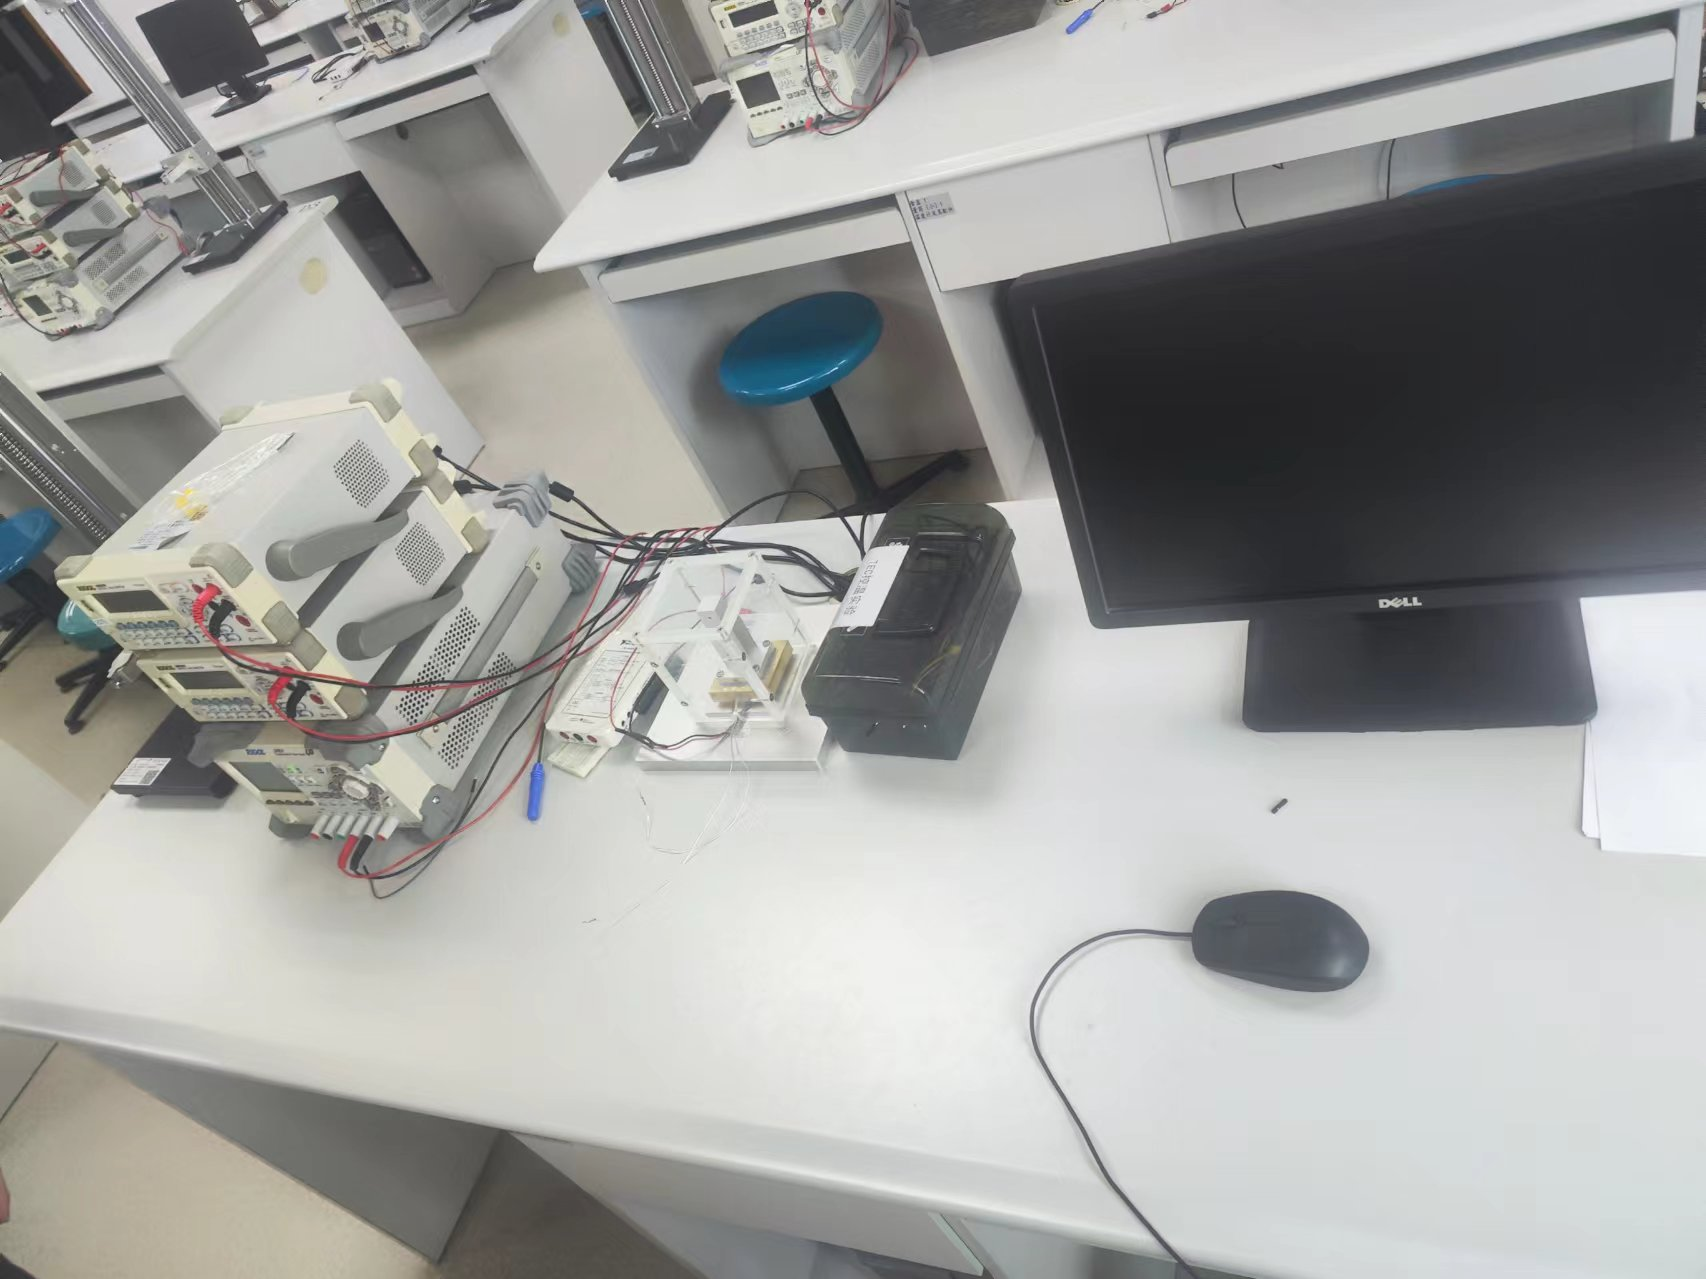
\includegraphics[width=0.4\linewidth]{桌面.jpg}
	
\end{figure}
	\begin{figure}[{H}]
		\centering
		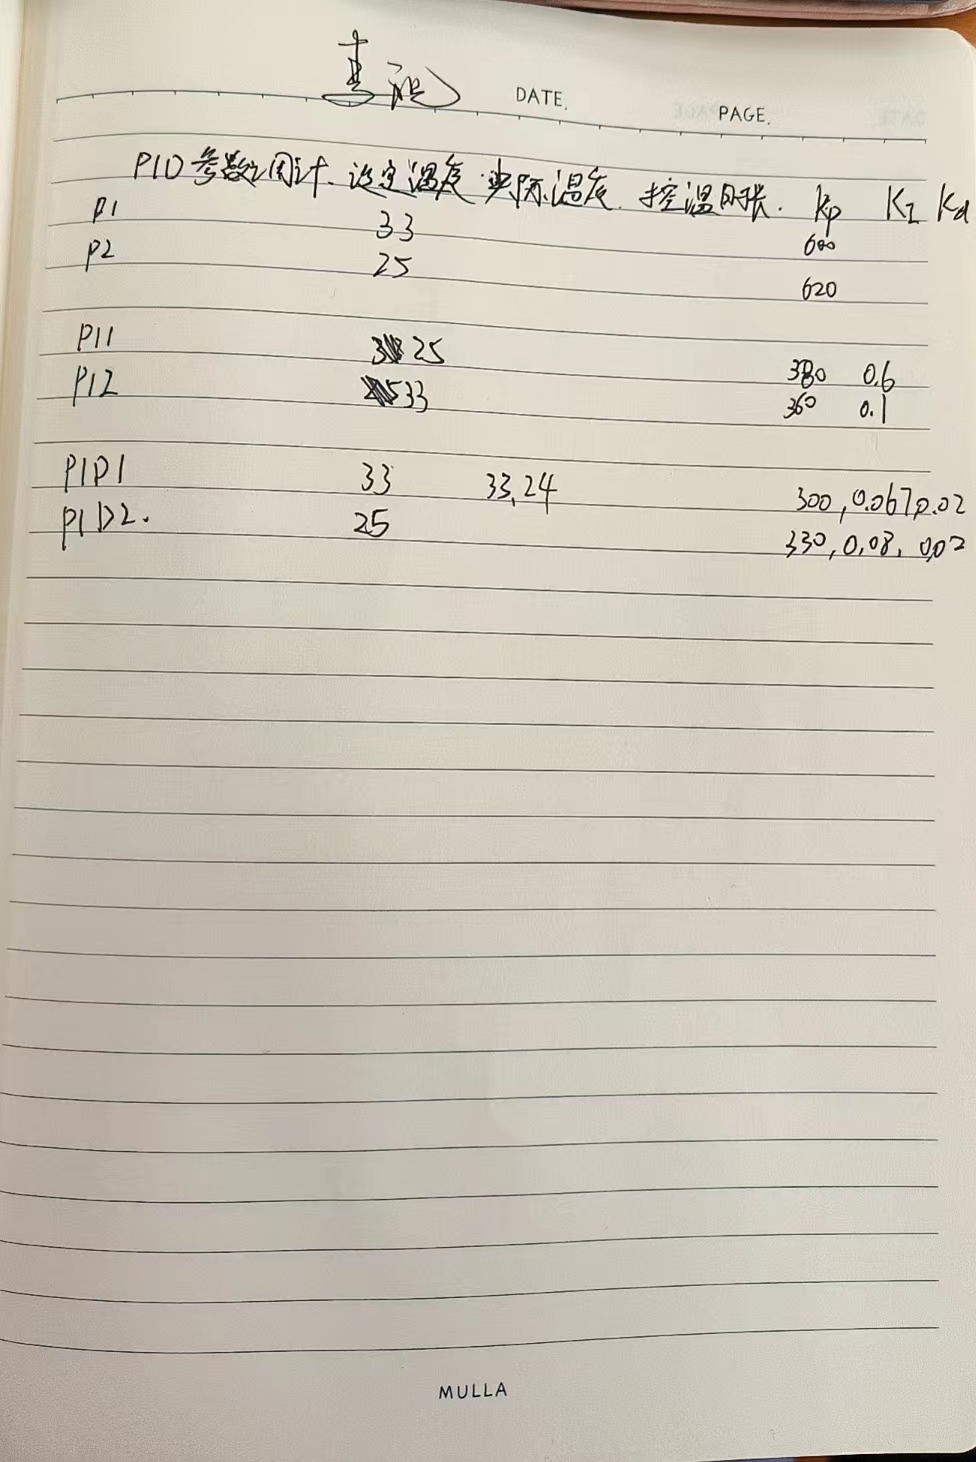
\includegraphics[width=0.2\linewidth]{原始.jpg}
		
	\end{figure}
	
\end{document}